\documentclass[11pt,a4paper]{article}

\usepackage[margin=1in]{geometry}
\usepackage{amsmath,amssymb,amsthm}
\usepackage{graphicx}
\usepackage[hidelinks]{hyperref}
\usepackage{booktabs}
\usepackage{enumitem}
\usepackage{tikz}
\usepackage{xcolor}
\usepackage{titlesec}
\usepackage[expansion=false]{microtype}
\usepackage{caption}
\usetikzlibrary{arrows.meta,positioning,fit,backgrounds,shapes.geometric,shadows}

\definecolor{abstrcol}{HTML}{2C5F8A}
\definecolor{numcol}{HTML}{D4850A}
\definecolor{boxbg}{HTML}{F5F5F5}

\titleformat{\section}{\Large\bfseries\color{abstrcol}}{\thesection}{1em}{}
\titleformat{\subsection}{\large\bfseries}{\thesubsection}{1em}{}
\titlespacing{\section}{0pt}{1.4em}{0.5em}

\newcommand{\abstr}[1]{\textcolor{abstrcol}{#1}}
\newcommand{\numr}[1]{\textcolor{numcol}{#1}}
\newcommand{\creed}[1]{\item \textbf{#1}}

\title{
\includegraphics[width=0.5in]{assets/logo-print.png}\\[0.75em]
       \textbf{openmaterials.ai}\\[0.3em]
       \large\normalfont Git for science: a versioned map of physics}
\author{The OpenMaterials project\\[0.25em]
        \small\texttt{openmaterials.ai}\ \ $\cdot$\ \ open source: map data
        CC~BY~4.0, code Apache~2.0}
\date{\today}

\begin{document}

\maketitle
\thispagestyle{empty}

\begin{abstract}
\noindent openmaterials stores the object a scientific result \emph{is}, not the
printout of it: a typed physical quantity, the executable formula that produces
it, its lineage, its units and gauge, and the codes that represent it. The map
doubles as a semantic layer for AI: fuzzy natural-language labels resolve to
typed, gated, content-addressed identities, so agents ground their language in
checkable physics instead of text similarity. This
document is the project's single source of truth. Part~I states the vision (why
science needs a git-like object model). Part~II describes the product (the free
protocol and the hosted app, the map, the parsers, the index, the contracts).
Part~III records the architecture (the operator and representation layers, the
two-worlds separation, the formal definitions, and the first thermal-transport
demonstration). Part~IV documents the implemented kernel (dimension algebra and
the dimensional gate, content identity, the log-first store, the frozen genesis,
and what remains). Part~V reports live status. The appendices carry the working
procedures for ingesting a code, extending the DAG, and encoding a catalog
skill.
\end{abstract}

\tableofcontents

\bigskip

% =====================================================================
\part{Vision}
\label{part:vision}
% =====================================================================

% ---- Hook ----
\noindent
Git did not just store files. It stored the \emph{repository}: a structured,
content-addressed object with identity and lineage, of which the working files
are one view. That object is why merging, provenance, and collaboration became
mechanical, and why a planet's worth of code could accumulate in one shared form.
Science is still pre-git. We ship the paper, the printout of a result, and throw
the object away. This is an attempt to store the object: what a result
\emph{is} (a typed physical quantity, its formula, its lineage, and the code that
produced it as one representation of it), so that results become reproducible by
construction, knowledge compounds instead of evaporating, and an AI agent has a
semantic place to act.

% ---- Creed ----
\section*{\color{abstrcol}The creed}
\begin{enumerate}[leftmargin=1.4em, itemsep=0.35em]
  \creed{The unit of scientific knowledge is meaning, not text.}
  \creed{Physics is the invariant. A code is one representation of it.}
  \creed{A scientific result is a structured object with identity and lineage, not a number in a table.}
  \creed{A result you cannot re-run is a claim, not yet knowledge.}
  \creed{Units, gauge, and lineage are part of a result, not footnotes to it.}
  \creed{Knowledge should compound, not evaporate into scripts.}
  \creed{Correctness should be structural, checked by the substrate, not re-derived by trust.}
  \creed{Verification must scale with compute, not with reviewers.}
  \creed{The native substrate for scientific AI is semantic, not token text.}
\end{enumerate}

\section{The problem: science that does not accumulate}

Computational materials science is a Tower of Babel. A single physical quantity,
say the lattice thermal conductivity of a crystal, is computed by a dozen codes:
kaldo, phono3py, ShengBTE, LAMMPS, VASP, Quantum ESPRESSO. Each has its own input
formats, its own unit conventions, its own gauge and basis choices, and its own
unspoken assumptions about what was held fixed. The physics is the same. The codes
never quite agree, and deciding whether two of them \emph{should} agree is itself
expert work.

That work does not accumulate. Reconciling two calculations is artisanal, done by
a handful of people who carry the conventions in their heads, and most published
computational results are effectively irreproducible because the real workflow
lives in tribal knowledge and one-off scripts rather than in the paper. The paper
is the tarball we email. Once it is sent, the object that produced it is gone.

\section{The diagnosis: meaning is implicit}

The reason the codes do not agree mechanically is that their meaning is implicit.
Scientific knowledge today lives in three forms, and each loses something. Prose,
in papers, carries rich meaning but does not run. Code runs, but its meaning is
entangled with implementation: the physics is mixed in with array layouts, loop
orders, and file formats. Data is numbers stripped of their provenance. None of
the three carries meaning that is at once machine-checkable and runnable.

So the physics is never stored directly. It is buried inside whichever artifact
happened to carry it, and recovering it, deciding what a given number actually
claims, is left to the reader. What cannot be recovered mechanically cannot be
checked mechanically, and so it cannot accumulate.

\section{The bet: store the physics, not the printout}

The move is to store the object. A result becomes a typed quantity, thermal
conductivity or a phonon frequency or a heat capacity, declared as what it is. The
formula that produces it rides on the edge that produces it, written symbolically
rather than implied by code, and the quantity carries its lineage, the ordered
chain of operations behind it, along with its units and gauge. A code is then no
longer the result; it is one \emph{representation} of it, a projection of a single
shared operator layer into one discretization and one set of conventions.

Every representation factors through that shared layer, never code to code. That
is what makes reconciliation mechanical: two codes that computed the same
observable are two projections of one object, so comparing them is a structural
operation on the graph rather than a feat of expert translation. It is merge, for
science.

\begin{figure}[h]
\centering
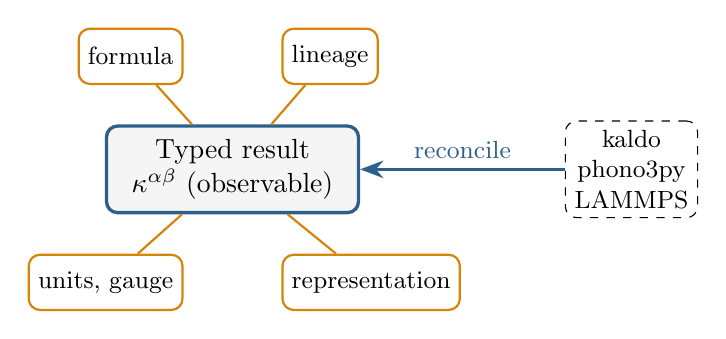
\begin{tikzpicture}[
  node distance=6mm,
  obj/.style={draw=abstrcol, very thick, rounded corners, fill=boxbg,
              minimum width=3.2cm, minimum height=1.1cm, align=center},
  tag/.style={draw=numcol, thick, rounded corners, fill=white,
              font=\small, align=center, minimum height=0.7cm},
  rep/.style={draw, dashed, rounded corners, font=\small, align=center}]

  \node[obj] (q) {Typed result\\$\kappa^{\alpha\beta}$ (observable)};
  \node[tag, above left=5mm and -1cm of q] (f) {formula};
  \node[tag, above right=5mm and -1cm of q] (l) {lineage};
  \node[tag, below left=5mm and -1cm of q] (u) {units, gauge};
  \node[tag, below right=5mm and -1cm of q] (p) {representation};
  \foreach \n in {f,l,u,p} \draw[numcol, thick] (q) -- (\n);

  \node[rep, right=2.6cm of q] (codes) {kaldo\\phono3py\\LAMMPS};
  \draw[->, >=Stealth, abstrcol, very thick] (codes) -- node[above, font=\small]{reconcile} (q);
\end{tikzpicture}
\caption{A scientific result as a structured object: a typed quantity carrying its
formula, lineage, units and gauge, with each code a representation that reconciles
into it at the observable. Merge, for science.}
\end{figure}

This is the same decision git made. A commit is identified by its content and its
parents; a result here is identified by its type and its lineage. Git won on its
object model, the blobs and trees and commits, not on its interface, and the
contribution here is the analogous object model for a scientific result. Getting
that object right is the whole game.

One difference is worth stating plainly, because it is where the real work lives.
Code is discrete and born digital, while a scientific result carries approximation,
continuous quantities, and gauge freedom: a per-mode lifetime depends on a basis
choice no two codes share, even though the conductivity it sums to does not. That
is why the object is typed, why units travel with it, and why the layer separates
\emph{observable} quantities, which must agree across codes, from
representation-dependent scaffolding, which need not. Defining what is allowed to
differ is as much of the design as defining what must match. The project already
ingests a \emph{code} this way; the vision is to ingest a \emph{paper} the same
way, turning its claims into objects the substrate can hold, re-run, and check.

\section{Proof it is real}

None of this is a promise about future software; the substrate runs today. Take
the lattice thermal conductivity of silicon. Computed through the operator graph,
it comes out directly in watts per meter per kelvin, with the unit conversion
applied automatically from the typed dimensions rather than pasted in by hand. The
same conductivity assembled along two different routes, the total on one side and
the sum of its population and coherence parts on the other, agrees to within about
$10^{-6}\,\mathrm{W/(m\,K)}$ on a value of order $100$, because the two routes are
views of one object and the substrate holds them to it.

The repository ships a smaller version you can run in seconds.
\texttt{examples/quickstart.py} builds the operator graph (54 quantities, 55
operators), derives the molar heat capacity of a crystal from a phonon frequency
array, $11.83\,\mathrm{J/(K\,mol)}$ at $300\,\mathrm{K}$, and cross-checks two
independent inputs at a gauge-invariant observable; the validation report returns
expected agreement with zero residual. This is merge, for science, and it already
runs.

\medskip
\noindent{\small The live operator graph is at
\href{https://openmaterials.ai/map}{openmaterials.ai/map}; the
architecture is Part~\ref{part:architecture} of this document.}

\section{The payoff: knowledge that compounds}

When results live as typed, reproducible objects, they stop being isolated. Each
one added to the graph makes the whole denser: a new code is a new representation
that can be checked against the others, and a new quantity opens new routes that
cross-validate the old ones. Reproducibility is the proof that a result was
captured faithfully; compounding is the dividend. The value is no longer locked in
any single paper but accrues in the shared, checkable object that all of them
project into.

This is the network effect git set off. Git made a standard object for code, and
on top of it grew GitHub, continuous integration, pull requests, and code review,
an entire ecosystem that exists because the object underneath was shared and
mechanical. A standard object for science invites the same: reproducibility
infrastructure, automated review, and a body of physics that grows more valuable,
and more trustworthy, with every result poured into it.

\section{The horizon: a semantic action space for AI}

There is a reason to care about this beyond tidiness. Today's models reason about
science in token space: they manipulate text that describes physics, and they
re-derive correctness from statistical pattern every time they are asked. That is
why a model can produce a fluent, confident, wrong step whose error only surfaces
three papers downstream. The substrate underneath is lossy, so the reasoning on
top cannot be trusted by construction.

A typed substrate offers a different footing: a semantic action space. An agent
that acts on the graph does not write a description of a calculation; it composes
an edge, materializes a quantity in a chosen code, contracts a hidden quantity into
an observable, cross-checks two routes. Each move is type-checked and dimensionally
sound by construction, so an invalid step becomes a type error rather than a silent
number. And because the routes are redundant, the substrate is its own verifier,
which is the scarce ingredient for reinforcement learning in any open-ended domain:
an agent can search and be told, mechanically, whether the answer holds.

The analogy closes the loop. The structured corpus of code that accumulated in git
is what made today's code models possible; a structured corpus of science is what
will let an agent reason over physics rather than over prose about physics. This
is, deliberately, Lean for computational physics, and like a proof assistant its
worth is that correctness is checked, not trusted. It is only partly built, but the
shape is already here.

\section{Where we are, and what is next}

Today the framework is real and growing. It has an operator layer and a
representation layer, 31 ingested representations (kaldo, phono3py, phonopy,
pymatgen, ShengBTE, Quantum ESPRESSO, VASP, LAMMPS, GPUMD, i-PI, the machine-learned
potentials matgl / MACE / fairchem, the database rail mp-api, and the CALPHAD,
amset, ORCA, OpenMM, and AtomisticSkills mat-* / chem-* workflows), and a
validation engine that executes the graph, composes
edges symbolically, and cross-checks redundant routes. Units reconcile
automatically from the typed dimensions, and a dimensional gate checks every
closed-form edge mechanically. The worked domains are lattice thermal
transport (54 quantities, 55 operators), the Quantum ESPRESSO DFT ground
state (the first contribution to land through the protocol gates), the
mechanics domain (the elastic tensor, its Voigt moduli, and the pressure), the
stability, thermochemistry, quasi-harmonic, molecular, and electronic-transport
domains (grown from the AtomisticSkills scans),
a first materials-diffusion subgraph, a thermodynamic-identities domain that
closes the map's formulas together, and a composites domain (composite effective
thermal conductivity with interfacial resistance); the unified map of
114 quantities and 114 operators is content-addressed in the log-first store
(Part~\ref{part:kernel}), grown past its frozen genesis version through the
contribution gates. Its dimensional layer is proven in Lean~4 against physlib
and recompiled in CI on every change to the map or its generators, its evidence carries pinned conformance
targets a re-run must reproduce, and the whole is held together by a suite of
1732 passing tests.

What is next is mostly upward and outward. The upstream from the
Born-Oppenheimer potential, the force constants from which everything descends, is
currently stubbed rather than modeled in full. The symbolic composition of error,
the approximation error carried by an operation and the discretization error
carried by a representation, is designed and not yet built. And the largest reach,
the one this document is really about, is to ingest not only codes but whole
papers: to turn a published result into an object the substrate can hold, re-run,
and check, the same way it already ingests a code. That reach has begun: the
paper parser already turns a PDF into gated, quote-anchored evidence proposals
and mints the share links that carry a whole paper's lineages; what remains is
scale.

\bigskip
\begin{center}
\color{abstrcol}\itshape
Git gave code a standard object, and an ecosystem grew on it. Give science the
same, and a result stops being a dead end: it becomes a contribution to a
compounding, machine-usable, verifiable body of physics.\\[0.5em]
\normalfont\bfseries The standard to store science.
\end{center}

% =====================================================================
\part{The Product}
\label{part:product}
% =====================================================================

\noindent
openmaterials is a versioned map of physics knowledge, built like git: typed
physical quantities (nodes) related by executable formulas (edges), every
element content-hashed, every change logged. The structure comes from codes and
theory: a respected codebase or a published derivation is what adds nodes and
edges. Experiments fill it in: each simulation run or measurement attaches a
value to a node, with its material, conditions, and source. Parsers turn the
world's codes, papers, and data files into both, and an index in the same
repository collects them. The map compounds: every code mapped and every value
attached makes the neighborhood more cross-checked, more reproducible, and more
trustable.

The picture has two tiers, the way git has GitHub. The \textbf{openmaterials
protocol} is free and open forever: the map format, the hashing rules, the
versioned change-log, the schemas, the parser contracts. The \textbf{openmaterials
app} is a hosted service on top: upload a map and see it rendered instantly, or
store your own custom and private maps. The protocol is the commons; the app is
convenience built on it.

\section{Protocol and app}

The protocol is a standard anyone can implement, self-host, and fork. The
mother map and its index are the shared artifact the community builds through
the protocol; they belong to no one and to everyone.

The app (the website, a separate project) adds the hosted conveniences: paste
and upload a map and have it rendered immediately in rich traversal views, the
way mermaid.live renders a diagram with no setup, and optionally store custom or
private maps. Anything hosted lives entirely app-side; it never touches the
protocol or the commons. The app is free while we build it, and how it is funded
later is out of scope here. The priority is the protocol and the map.

The priority is explicit: first build the community that builds the mother map,
and a rich initial map worth using. The app comes second. Protocol adoption is
what makes the app valuable, the same way git had to matter before GitHub
could.

The site already carries a first taste of the app: a Learn page that runs the
paper parser as a public demo. Because that demo calls a paid model, it runs
through a cost-gated Cloudflare Worker (\texttt{infra/learn-proxy}) rather than
from the browser: the Worker holds a daily budget and per-IP limits and keeps the
API key server-side, never shipping it to the page. The Learn page is also a
contributor on-ramp: a value a reader accepts from the parser's output is
exported as an instance JSON in the committed schema, with a prefilled GitHub pull
request link, so contributing a value from a paper is one reviewed PR through the
same gates the maintainers use.

\section{Structure and evidence}

Two kinds of thing live on the map, and they come from different places. This
is the load-bearing distinction.

\textbf{Structure} is nodes and edges. It comes from \textbf{sources}: a code (the kaldo,
QE, or LAMMPS codebase) or a theory paper. A source asserts that a quantity
exists and that a formula relates it to other quantities. Codes are the ground
truth we seed from, because a respected code is an executable statement of the
physics; theory papers and, later, new derivations extend the structure.

\textbf{Evidence} is values on nodes. It comes from \textbf{instances}: one
committed value, computed or measured. An instance attaches a value to a node,
with the material, the conditions, and a citation (a whole run is the separate
simulation record). Evidence never creates structure: a
simulation cannot invent a formula, it can only put a number on a node that
already exists.

The split is also a separation of concerns in the app. The map view renders the
structure alone (nodes, edges, formulas, and the code representations that map
onto them); the four data record kinds beside the ledger (instances,
configurations, spectra, and simulations) are a distinct evidence layer that
consumers load against node uids and attach locally, never carried on the map
page itself.
The test suite and the contribution gates exercise that layer directly, so its
correctness is checked against the same uids the view is drawn from.

The two relate through a small type hierarchy. A code is a \textbf{representation}: a
named mapping of part of the map onto a concrete tool, with its units, gauge,
and conventions. One committed value that code produced is an \textbf{instance}:
the kappa a run outputs is a \textbf{value on the kappa node}. A growth process such as CVD is an
experiment type, also a representation; a specific synthesis and measurement is
an instance; its measured number is a value on a node. So ``is ShengBTE a tag?''
resolves cleanly: ShengBTE is a representation, a ShengBTE run is an instance,
and its result is a value on a node.

One name per concept is enforced throughout this document. The canonical terms,
and the near-synonyms they subsume:

\begin{center}
\small
\begin{tabular}{lll}
\toprule
Concept & Canonical term & Notes \\
\midrule
A typed quantity on the map    & \textbf{node} & \texttt{Space} is the code class. \\
A relation producing a node    & \textbf{edge} & \texttt{Operator} is the code class. \\
A code's mapping onto the map  & \textbf{representation} & its on-map rendering is a \emph{rail}. \\
A committed value               & \textbf{instance} & the \texttt{\{id, kind, lineage, source\}} record. \\
A semantic type parameter       & \textbf{label} & e.g.\ \texttt{bte\_solver=rta}, not a ``variant''. \\
A content hash                  & \textbf{uid} & sha256; a 12-hex prefix is displayed. \\
\bottomrule
\end{tabular}
\end{center}

\section{The map}

The map is a curated reference graph. Today it holds 114 nodes (111 observable
and hidden quantities plus 3 promoted parameters) and 274 edges. Nodes are
typed physical quantities. An edge produces one node from a list of input
nodes, carrying the symbolic formula that relates them (parameter inputs are
marked as inputs rather than derived through a formula).

Identity is structural plus one curated semantic tag. A node's id is the hash
of its quantity tag, its field signatures (dimension and index kinds per
field), its gauge class, and its labels; an edge's id is the hash of its output
and input node ids, its formula fingerprint, and its schemes. The quantity tag
exists because physics is full of same-typed distinct quantities (entropy and
heat capacity share dimension, indices, and gauge); tags, index kinds, labels,
and gauge groups live in small controlled registries that are part of the
protocol. Names and symbols are not part of identity, so your \texttt{kappa} and my
\texttt{k\_L} are the same node when you both map to the registered quantity, and a
formula written \texttt{c v\^{}2 tau} or \texttt{tau v\^{}2 c} is one edge because both normalize
to the same fingerprint. Genuinely different decompositions stay separate
graphs and are reconciled where they meet, at a shared observable; production
routes are never part of a node's identity, so adding an alternative
derivation of an existing quantity never re-mints the node. The consequence is
that two people who contribute the same physics converge through the shared
registries, while a real difference in decomposition surfaces as a parallel
route rather than a false merge. The implemented form of these rules, with the
collision rationale that forced the quantity tag, is Part~\ref{part:kernel}.

Three properties propagate, rather than being hand-stamped on every node:

\begin{itemize}[leftmargin=2em]
  \item \textbf{Units} live on leaf nodes and propagate through operations; a derived
  node's units are computed, never stored.
  \item \textbf{Gauge} lives on index kinds. Mode and branch indices, and the phase of an
  eigenvector, carry a representation's gauge freedom; a node is \textbf{observable}
  once every gauge-carrying index has been contracted away, and \textbf{hidden}
  until then. Cross-source values may be compared only at observables.
  \item \textbf{Symmetry} lives on index kinds too. A quantity's intrinsic index symmetry
  (the thermal-conductivity tensor satisfies $\kappa^{ab} = \kappa^{ba}$) belongs to
  the node; a material's crystal symmetry (cubic silicon making $\kappa$ isotropic)
  acts on the spatial indices at the material and instance level, not on the
  node. Symmetry is what proves that one code reporting $\kappa_{xx}$ and another
  reporting the trace over three are reporting the same observable.
\end{itemize}

The map is versioned like git, log first. The change-log is the map: an ordered
sequence of operations (add, edit, or deprecate a node; add or remove an edge;
supersede an element), each carrying a date, a reason, and an author. A
materialized current version is always kept in sync, so reading the map is
immediate. The map version hash chains the log, computed as the hash of the
previous version hash combined with the new change record, which makes the
history tamper-evident and path-dependent. Because identity is structural,
editing a foundational leaf re-mints every node above it (a Merkle ripple); the
supersede record ties the old subgraph to the new one. The design gives a
value two currencies, stay pinned for reproducibility or follow the supersede
chain; today the committed records carry no pin, and the regenerated
projection stamps each value with the live node uid, so published values
follow the current map.

Provenance and confidence ride on every element. A node or edge records the
sources that assert it (which codes and papers) and accumulates the instances
that put values on it. Many independent instances are a confidence signal, but
independence is not the same as multiplicity: two solvers run on the same
interatomic potential are not independent confirmations, so the map keeps the
full provenance (potential, method, code) and lets independence be judged rather
than counting raw repetitions. A claim no instance has reached yet still lives
on the map, simply unconfirmed.

\section{The semantic layer}

The map speaks symbolic language: typed nodes, executable formulas, proven
dimensions. The literature and the language models that read it speak semantic
language: labels like ``quasi-harmonic approximation'' or
``phonon-thermal-conductivity''. The semantic layer (2026-07-12) connects the
two as a first-class artifact: every node and edge carries its cloud of surface
labels (auto-derived forms plus a curated alias registry, reviewed like
vocabulary), published uid-pinned in \texttt{docs/data/semantics.json} and
regenerated with the map. A deterministic resolver turns any fuzzy label into
ranked typed identities: normalization, exact alias hits, token containment,
no embeddings, so every resolution is auditable. An agent that grounds its
phrase through the resolver inherits everything the map knows about the
element: the formula, the dimensional proof, the producing codes with their
citations, the evidence with its provenance. A label that resolves to nothing
is an honest coverage gap and feeds the encode queue. External method
vocabularies (the first being a 16,012-paper skill map extracted by
large-scale literature analysis) will align to the map through reviewed
alignment files, each unmatched label ranked by its usage frequency in the
field; today the curated aliases carry that role while the corpus is awaited. This
is the sense in which the map is a semantics for AI: fuzzy language in,
checkable identity out.

\section{The parsers}

A parser is an assisted on-ramp, one per artifact type. Each proposes
structure, values, or both; the map validates them; a human confirms. One of the
three exists today; the other two are designed and not yet built.

\begin{itemize}[leftmargin=2em]
  \item The paper parser turns a paper's measured or computed numbers into values
  on nodes (and, in its eventual full form, its formulas into edges). Its
  value-extraction half is built (\texttt{omai/paper\_parser}, gated evidence),
  detailed under the parser contract below.
  \item The code parser will import a codebase as a representation: mapping the
  code's input, output, and intermediate files and key lines onto the nodes and
  edges the code implements (structure), and letting a run of the code be recorded
  as an instance (values). The 31 representations on today's map were authored by
  hand against this contract; the parser that automates the mapping is not yet
  built.
  \item The run parser will read a concrete run and record its inputs (from the
  input file) and its outputs as values on the nodes they belong to.
\end{itemize}

Proposals must pass the map's types as continuous integration: dimensional
agreement; reachability, so a value lands only on a node that already exists and
a new edge is introduced only by a code or a theory source, never by a bare
experiment; observable discipline, so cross-source equality is asserted only at
observables; completeness, so every input and output of a run is recorded; and
coherence, so one source's contributions form a connected subgraph. All the
difficulty of joining the commons concentrates here, in the parsers, which is
what keeps the store itself simple.

\section{The index}

The index is a subfolder of the map repository, in two clearly separated parts.

The canonical registry is organized by source: \texttt{papers/}, \texttt{codes/},
\texttt{experiments/}. Each entry holds that source's structure contributions and the
values its instances produced, pinned to a specific element hash at a specific
map version.

The derived lookups are regenerated from the registry and the map, never edited
by hand: symbol to node, value to instances, source to coverage.

One clone gets you the map and the world's evidence together.

\section{Contracts (for builders)}

These are the interfaces the protocol defines. The store, index, and identity
contracts below are implemented (Part~\ref{part:kernel}); of the parsers, the
paper parser's value-extraction half is built and the code and run parsers remain
the eventual on-ramp, each its own spec, plan, and build cycle.

\paragraph{Store operations.} \texttt{push(change)} appends a change record (op, target, date,
reason, author) and advances the version hash. \texttt{read()} returns the
materialized current map. \texttt{read(hash)} returns the map at a given version.
\texttt{diff(hashA, hashB)} returns the change records between two versions. Identity
is by content: a node id $=$ hash(quantity tag, field signatures (dimension $+$
index kinds per field), gauge class, labels); an edge id $=$ hash(output ids,
input ids, formula fingerprint, schemes); the version hash $=$ hash(previous
version hash $+$ change record), unchanged (quantity tags, index kinds, labels,
and gauge groups live in controlled registries).

\paragraph{Structure contribution (from a source).} A code or a theory paper proposes
new nodes and edges. Inputs to any new edge must resolve to nodes that already
exist or are introduced by the same source in the same contribution, processed
in dependency order. Reviewed before it lands in the canonical map.

\paragraph{Value record (a lineage instance).} A committed value is a
\emph{lineage instance}: one construct, \texttt{\{id, kind, lineage, source\}}.
The \texttt{lineage} is the complete computational identity of the value: the
node, the material, every condition that determines the number, and the values
block. \texttt{id} is the sha256 of the lineage's canonical JSON, so two
records with the same id are the same computation, and any change to the
canonicalized lineage (floats are rounded to six decimals before hashing, so
re-serialization noise never re-mints) yields a different id. The implemented schema, shown as the committed
instance, with the one long \texttt{detail} string wrapped for print
(\texttt{docs/data/instances/si-thermalconductivity-bte-solver-rta-kaldo.json}):

{\small
\begin{verbatim}
{
  "id": "04c6dbdb9b046aceefb0c7b44e4219574cb2259280bc6893c0180b620fbcea52",
  "kind": "simulation",
  "lineage": {
    "node": "ThermalConductivity[bte_solver=rta]",
    "material": "Si",
    "conditions": {"T": 300, "mesh": "8x8x8", "potential": "Si.tersoff"},
    "values": {"value": 19.46, "units": "W/(m K)"}
  },
  "source": {
    "kind": "simulation",
    "ref": "kaldo",
    "detail": "RTA; Tersoff; 8x8x8 mesh (cross-code meaningful,
               absolute under-converged)"
  }
}
\end{verbatim}
}

\texttt{lineage.node} always names a node, because a value belongs to a
quantity; at bundle time each record is additionally pinned to that node's
content uid (\texttt{node\_uid}, injected into the flat, regenerated projection
\texttt{docs/data/instances.json}, never into the hash). A lineage may also
carry its own \texttt{source} as a namespaced \texttt{scheme:ref} string
(\texttt{paper:...}, \texttt{doi:...}, \texttt{zotero:...},
\texttt{arxiv:...}; the scheme set is open), and that in-hash source is
identity-bearing: the same claim from the same source mints the same id, while
one paper's claim and another paper's identical number stay distinct records.
The top-level \texttt{source} block is display provenance and rides outside
the hash forever; a record whose two sources conflict is malformed. The
material is deliberately NOT part of the map's
structure: the map's nodes are quantities of physics in general, and the
material enters only here, on the value, as the point where the quantity was
evaluated (with \texttt{conditions} carrying the rest of the evaluation
point). A value record never introduces structure; that is a separate,
reviewed contribution through the gates.

\paragraph{Configuration record (structure-valued evidence).} The
\texttt{Structure} node is one opaque node on the map, but a value of it is a
periodic atomic configuration: lattice vectors, fractional coordinates, and
species. That payload lives in a configuration record, the structural sibling of
the value record. It is content-addressed by a canonical uid: the sha256 of the
spglib-standardized primitive cell (\texttt{symprec} $10^{-3}$), origin-anchored
so a rigid translation is invariant, with species and sites sorted and
coordinates rounded to five decimals (a hundredth of a milliangstrom: coarse enough to absorb refetch-level numerical noise, fine enough that physically distinct cells never collide; the matcher gate reviews the boundary). The same cell, its sites shuffled, and a
supercell of it therefore hash to one uid; a strained cell does not. On top of
the hash a validation gate runs \texttt{StructureMatcher}: a
physically-equivalent but not hash-identical cell is flagged for human review
rather than silently merged, and provenance appends to the one record on a
confirmed duplicate. The implemented schema, shown as the first committed record
with the site list elided
(\texttt{docs/data/configurations/si-diamond-primitive-mp-149.json}):

\begin{verbatim}
{
  "name": "Si diamond primitive (mp-149)",
  "formula": "Si",
  "natoms": 2,
  "structure": { ...pymatgen Structure.as_dict()... },
  "canonical": {
    "uid": "55bf22ca8186...",
    "spacegroup": 227,
    "natoms_primitive": 2
  },
  "external_ids": {"materials_project": "mp-149"},
  "provenance": [
    {"kind": "database", "ref": "materials-project",
     "detail": "mp-149, GGA-relaxed primitive cell"}
  ],
  "files": null
}
\end{verbatim}

The record is pinned at bundle time to the \texttt{Structure} node's content uid,
the same \texttt{node\_uid} discipline a value record follows, so a configuration
travels with the node through supersede chains. Cells at or below 1000 atoms
embed the full structure dict inline; larger cells (a 17k-atom amorphous cell)
point to a committed structure file and keep only reduced metadata inline so the
record stays searchable. A value record may now carry an optional
\texttt{configuration} key naming this uid; \texttt{material} stays the display
string, so the addition is backward compatible and the existing instances are
untouched. This is where the structure-ish numbers a run reports (atom count,
cell volume) belong: not as scalar evidence on their own nodes, but as derived
views of a configuration.

\paragraph{Spectrum record (function-valued evidence).} Some nodes are
function-valued in practice (a phonon density of states, a diffraction pattern,
a dielectric function): the evidence is not one scalar but an array of ordinates
against a monotonic axis. A spectrum record keeps the flat pre-lineage shape
(its migration to the lineage construct is pending): the scalar is replaced by
an axis and an array, attached to the same nodes and pinned the same
way (\texttt{node\_uid} at bundle time). Each spectrum-capable node's
representation declares a \emph{canonical axis} (a registered unit and its
dimension) so the axis and value units can be validated against a fixed
convention; the axis must be strictly monotonic and the arrays equal-length.
The implemented schema, shown as a real committed record with the long arrays
elided
(\texttt{docs/data/spectra/li-phonondos-mat-phonon.json}):

\begin{verbatim}
{
  "variable": "PhononDOS",
  "material": "Li",
  "conditions": {"structure": "BCC",
                 "model": "TensorNet-MatPES-r2SCAN-v2025.1-PES",
                 "supercell": "3x3x3",
                 "normalization": "states/THz per unit cell"},
  "axis": {"name": "omega", "units": "linear_THz",
           "values": [-0.771482, -0.724914, ..., 8.542130]},
  "values": [0.0, 0.0, ..., 0.0],
  "units": "states/THz",
  "uncertainty": null,
  "source": {
    "kind": "simulation",
    "ref": "mat-phonon",
    "detail": "AtomisticSkills mat-phonon Li BCC example, total_dos.dat
               verbatim (201 bins, linear THz axis) ..."
  }
}
\end{verbatim}

The DOS density carries no registered unit: its normalization (per cell versus
per formula unit) rides in \texttt{conditions}, so the canonical axis pins the
frequency axis and leaves the ordinate unit open. Diffraction is deferred: the
XRD pattern's canonical axis (the wavelength-free plane spacing $d_{hkl}$, with
the radiation wavelength a required condition of any served $2\theta$ axis) is
recorded as a representation note, and a spectrum against it becomes admissible
only when an \texttt{XRDPattern} node is minted.

\paragraph{Simulation record (a light, lineage-identified, URL-first run).} The
value, configuration, and spectrum records each capture one number, one cell, or
one curve; a \emph{simulation record} captures a whole experiment, and it is
deliberately \emph{light}: it stores whatever we have, with no fixed
reproducibility guarantee and no required heavy input files. Its core is the
\texttt{lineage}: the map node when one is known (with a content-uid pin), else a
\texttt{template} with its \texttt{hyperparameters} and setup \texttt{values},
plus \texttt{material}, \texttt{conditions}, and \texttt{params}. Identity is the
lineage alone, content-addressed by the sha256 of its canonical JSON with the same
float-rounding discipline the configuration uid uses. Everything else rides
\emph{outside} the hash: an optional \texttt{execution} block (code, version,
seeds, wall time, whatever the run recorded); optional \texttt{artifacts}, which
are pointer-only, each \texttt{\{path, role, url?, sha256?\}} where only path and
role are required and the url points at the heavy bytes on MaterialsCodeGraph
(MCG), the cheap host, never embedding them; a \texttt{mirrors} resolver; and the
run's \texttt{results}. Attaching a trajectory pointer, moving its bytes, or
re-running on another node therefore never re-mints the record. Because the
record is light, it is URL-encodable: gzip and base64url pack it into a
\texttt{\#x=} link fragment that opens in the openmaterials playground and, when
the lineage names a map node, lights that node on the map, so an experiment is a
link, no server, that carries the lineage and its receipts together. The get is
that link; the heavy bytes are a separate, optional enrichment. A record with no
artifacts and no map node is valid and normal: validation resolves a node by id
and uid when the lineage names one (a stale pin is a mismatch, never a silent
pass), and simply flags node-unresolved otherwise rather than rejecting it (the
honesty rule). A full, checksummed bundle from MCG can additionally enrich a
record with verifiable byte pointers, which a verification tool then checks
against their checksums as a dated report, never a gate; but that heavy path is
optional and never required for a record to exist or to have identity. This is
the same bytes-out-of-git rule the governance commits to (the open format holds
the lineage and its identity, the platform holds the artifacts, referenced by
pointer), made into a first-class record kind.

\paragraph{The share envelope (multi-lineage bundles).} A parsed paper rarely
yields one lineage, so the \texttt{\#x=} wire carries an \emph{envelope},
\texttt{\{v: 1, doc, lineages: [...]\}}: shared document metadata
(\texttt{doc.source} as a \texttt{scheme:ref}, plus title, authors, year,
journal) and one or more lineage records, gzip-compressed and
base64url-encoded into the fragment. The reader is dual forever: a bare single
record decodes as a one-element envelope, so every link minted before bundles
keeps rendering unchanged. A bundle opens as one page of stacked datasheets,
one per lineage, each with its derivation drawn as an excerpt of the map;
\texttt{doc.source} is inherited by members at read time for display only,
never hashed into any member's id. The bundle itself is content-addressed
(\texttt{bundle\_id}: the sha256 of the canonical document metadata plus the
member ids in order). A link that would exceed 8000 characters is refused with
a download-the-JSON fallback rather than silently truncated: the honesty rule,
applied to the wire.

\paragraph{Conformance target (a pinned expectation).} The check side of the
evidence. A target is \texttt{\{id, lineage, code, expected, tolerance,
evidence?\}}: the number a named code is expected to reproduce for one
committed computation, within a stated absolute or relative tolerance. A
target never invents its lineage: it carries the evidence instance's lineage
verbatim, so the hash of \texttt{target.lineage} equals \texttt{target.id}
equals the instance's id, a cryptographic not-invented proof rather than an
asserted link, and \texttt{expected} mirrors the instance's own values. (A
literature target may carry no evidence instance; its lineage then names a
\texttt{doi:} or other \texttt{scheme:ref} source in-hash, and the citation
itself is the provenance.) The
committed targets are projected into a byte-stable index that the playground
datasheets read: a record's page lists, under \emph{Reproduce this}, the codes
that can compute its quantity and the pinned runs for its node, with a target
whose id equals the record's id marked as the same computation. The first
engine-adapter targets (kaldo and phono3py silicon thermal conductivity, every
knob pinned in-hash down to the sha256 of the potential file) landed
2026-07-18.

\paragraph{Parser contract.} Input: one artifact (a codebase, a paper, a run). Output:
proposed structure and value records. Every proposal must pass validation below
before a human confirms it into the index.

\paragraph{The paper parser, implemented.} The first parser exists:
\texttt{omai/paper\_parser} turns a PDF into a gated evidence proposal in six
stages. INGEST extracts the text with page offsets. DETECT enumerates every
reported value with a verbatim, page-located quote through a citations-enabled
model pass, run as an ensemble: a single pass is unreliable (its recall swung
between $0.375$ and $0.875$ across runs because one pass can miss values), so
three independent passes with diverse prompts (a broad sweep, a table/caption
sweep, a prose sweep) are unioned, two claims counting as one finding when they
share a normalized value, a compatible quantity name, and an overlapping quote or
adjacent page. MAP aligns each detected value against the node catalog via
structured outputs; a claim that lands on a source or parameter node
(\texttt{Structure}, \texttt{Temperature}, \texttt{AtomCount}, and the rest of
the input set, flagged \texttt{evidence\_target: false} in one place in the
catalog builder) is classified as a run \emph{condition}, not a value. Printed
numerals are normalized before the value gate (thousands separators, the
comma-space artifact of a line break, the unicode minus, and $a \pm b$ forms,
whose central value is the claim), because PDF extraction mangles real numbers
into shapes a bare parser rejects; on the first paper this recovered the three
known claims that formatting alone had killed. Such
claims survive into the proposal as context and are counted separately, but are
excluded from instance minting at apply time: an atom count or a temperature is a
condition of a run, whose structural home is the configuration record and the
\texttt{conditions} field, never a scalar instance on its own node. VALIDATE runs deterministically over the kernel, killing any
claim whose quote is not found verbatim in the document (the hallucination gate)
and flagging values that duplicate a committed instance. REVIEW is an adversarial
model pass. PROPOSE emits a proposal file that a human confirms with
\texttt{--apply} before any instance is written. The pipeline never prints or logs
the API key. It is golden-evaluated against this very document, against a
committed expected set of eight values: the acceptance bar is recall $\ge 0.8$
with the worst of the ensemble runs still clearing it, no hallucinated quote
surviving validation, and every recovered known correctly flagged as a duplicate
of its committed instance. The ensemble was built to hold that recall bar against
the single-pass variance, which is the honest edge of a model-driven extractor.

\paragraph{Index schema.} Registry: \texttt{index/papers/}, \texttt{index/codes/},
\texttt{index/experiments/}, each entry pinned to (element hash at map version).
Derived files (regenerated, never hand-edited): symbol-to-node,
value-to-instances, source-to-coverage.

\paragraph{Validation rules.} Dimensional agreement on every edge. Reachability: a value
lands only on an existing node, and a new edge is introduced only by a code or
theory source. Observable discipline: cross-source equality is asserted only at
observables. Completeness: every input and output of a run is recorded.
Coherence: a single source's contributions form a connected subgraph.

\section{Governance}

The protocol is forkable: anyone can self-host a map or fork the mother map.
Landing a contribution in the canonical maintained repository goes through a
reviewer list. Content-addressing handles identity and deduplication on its own;
the reviewers decide what enters the commons.

\section{Status and build order}

Today's map is one hundred thirty-nine change records past v1, its frozen genesis version:
111 typed quantities plus 3 promoted
parameters, the symbolic formula on every relational edge, 31 representations
mapped (kaldo 34 variables, phono3py 31, phonopy 22, pymatgen 22, ShengBTE 20,
mp-api 13, QE 13, LAMMPS 12, VASP 10, GPUMD 8, pycalphad 7, i-PI 4, and a further
nineteen codes and mat-* / chem-* skills at five or fewer each), and real instances
computed through the framework: cross-code silicon thermal conductivity
(Tersoff potential, 8x8x8 mesh, 300 K: kaldo 19.46 RTA and 26.91 direct,
phono3py 16.74 RTA and 24.30 direct, in W/m K) plus an LGPS activation energy
(0.152 eV) from the materials domain. It is live and browsable as an
interactive map.

The contributor on-ramp today is curated pull requests reviewed by the
maintainer list; the silicon values above arrived that way. The genesis
version hash is now frozen and the log-first store and the index exist, so the
map's source of truth is data (an append-only log plus a materialized view) and
the Python operator layer is an authoring client that emits change records;
Part~\ref{part:kernel} documents all three. The parsers are the automated
on-ramp, not the day-one one: the paper parser's value-extraction half now
exists, and the code and run parsers remain the next build after the store and
index.

\section*{See also}

\begin{itemize}[leftmargin=2em]
  \item The vision, why this matters: Part~\ref{part:vision} (Part~I of this document).
  \item The architecture, how the operator and representation layers work:
  Part~\ref{part:architecture} (Part~III of this document).
  \item The map, live: \texttt{docs/map/} (openmaterials.ai/map).
  \item The codes bibliography, every cited code with its interface, citation,
  and license: \texttt{docs/codes/} (openmaterials.ai/codes).
  \item The verified layer and its roadmap, live: \texttt{docs/lean/}
  (openmaterials.ai/lean and /lean/roadmap/).
  \item This document, browsable with a PDF download:
  \texttt{docs/document/} (openmaterials.ai/document).
  \item The deck, a short walkthrough: \texttt{docs/deck/}.
\end{itemize}

% =====================================================================
\part{The Architecture}
\label{part:architecture}
% =====================================================================

\noindent This part records the design of the typed operator/representation
framework: the two-worlds separation, the formal definitions, the gauge
discipline, and the first thermal-transport demonstration. It is carried from
the standalone architecture reference essentially verbatim; the implemented
kernel that supersedes its content-identity and store sketches is
Part~\ref{part:kernel}.

\section{Principles}
\label{sec:principles}

The operator layer is built on a small set of commitments. They are stated here without
their alternatives or justifications; supporting definitions follow in later sections.

\begin{enumerate}[leftmargin=2.5em, itemsep=0.4em]
  \item \textbf{Two worlds, one bridge.} The operator layer keeps the operator physics world
        (typed states, operator operations, approximation errors) strictly separate from
        the numeric world (discretized arrays, computed values, discretization errors).
        They are connected by exactly one bridge: the representation functor.

  \item \textbf{Operator states are unit-free.} Dimensionful quantities (frequency,
        energy, length, time) exist at the operator layer, but specific unit choices
        (THz vs eV vs rad/s, \AA{} vs Bohr) do not. Unit choice belongs to the
        representation and is declared by the adapter that produced it; the framework
        normalizes to a canonical unit before any cross-representation comparison.

  \item \textbf{The atom is an operator operation.} The atomic unit of meaning is a typed
        transformation between operator states, not an instruction in an input file or an
        algorithm. Every operation carries a \emph{operator formula}---a sympy expression
        (closed-form output) or sympy.Eq (implicit equation defining the output)---stating
        what it computes. The formula is the operator claim, machine-readable and
        Lean-projectable, against which adapter conformance can be checked.

  \item \textbf{States are typed witnesses; nodes are ObservableSpaces or HiddenSpaces.}
        A state is the typed claim that an operator physics object exists with a
        particular history. The operator layer splits states into two structural kinds:
        \emph{ObservableSpaces} (gauge-invariant, first-class, required to agree across
        adapters) and \emph{HiddenSpaces} (gauge-dependent intermediate scaffolding
        whose per-element values reflect basis / phase / BZ-summation choices the
        framework does not pin down). Each state declares fields, and each field has an
        index signature (e.g.\ $\omega(\mathbf{q},\nu)$ has indices $(\mathbf{q}, \nu)$;
        $\kappa^{\alpha\beta}$ has $(\alpha, \beta)$). Numerical content lives in the
        representation, separate from the witness.

  \item \textbf{Workflows are directed acyclic graphs.} A workflow is a graph of states
        connected by operations, not a linear sequence. Cross-code comparison reduces
        to graph alignment over the same operator template.

  \item \textbf{Identity is content, not history.} A operator state is identified by its
        \emph{content}: the quantity tag plus the type content (its field
        signatures, meaning each field's dimension and index kinds) plus its
        gauge class plus its labels. Provenance refers to a quantity instance's
        \texttt{source.ref}; a lineage is the shareable run record. Neither is part
        of a node's identity: production routes are recorded but a route never re-mints
        a node, so adding an alternative derivation of an existing quantity leaves
        the node's id unchanged. The implemented form of this rule, with the
        collision rationale that forced the quantity tag, is Part~\ref{part:kernel}.

  \item \textbf{Operation identity is parameterized.} An operation is identified by its
        name together with the parameters that affect physics. Different physics-affecting
        parameter values produce different operations and therefore different output
        states. Function-family parameterizations (e.g., Gaussian broadening by standard
        deviation vs.\ by half-width) are canonicalized at the operator layer to a single
        choice; adapters translate to their internal convention.

  \item \textbf{Discretization belongs to representation.} Mesh densities, supercell
        sizes, displacement steps, and broadenings live on the representation, not on
        the operator state. Convergence is a relationship between an operator state and
        a family of its representations.

  \item \textbf{Cross-code agreement is required at ObservableSpace nodes only.} Two
        adapters' representations of an ObservableSpace must agree (after unit and
        normalization conversion) to within the observable's declared tolerance.
        Representations of a HiddenSpace are not cross-code comparable per-element;
        the operator layer's \texttt{compare} returns the status \texttt{NOT\_COMPARABLE}
        and reports residuals as diagnostic information only. To make a HiddenSpace
        cross-code comparable, contract it into an ObservableSpace (e.g., per-mode
        $\Gamma_{q\nu}$ is a HiddenSpace; $\sum_{q\nu}\Gamma$ contracted via the
        BZ sum is an ObservableSpace that does agree).

  \item \textbf{Errors are designed-for.} Approximation errors live on operations;
        discretization errors live on representations. The type system reserves slots
        for both; operator composition of error formulas is a Phase~2 capability.

  \item \textbf{The operator root is the potential.} Every representation in the framework
        ultimately traces back to the Born--Oppenheimer potential of the material. Force
        constants of every order are derived states obtained by extracting derivatives of
        the potential and truncating the Taylor expansion. The upstream is stubbed in
        Phase~1.

  \item \textbf{Sources are produced by nullary operations.} Source states (the
        potential, but also temperature, lattice constant, etc.)\ are the outputs of
        nullary \texttt{provide\_*} operations rather than nodes with empty provenance.
        This unifies the DAG: every node is the output of some operation, and the
        operator layer has no special ``input'' category. The representation of a source
        state carries the externally supplied value (e.g., $T = 300\,\mathrm{K}$); the
        operation is just a structural tag.

  \item \textbf{Lean-compatible by structure.} The operator layer is implemented in Python
        but designed so that its types transliterate cleanly into Lean. Three disciplines
        protect this option: closed unions for physics types, no Python-encoded physics
        invariants, operation parameters always recorded in output state metadata.
       
\end{enumerate}

\bigskip


\section{Background and Motivation}
\label{sec:motivation}

Modern computational materials science has many codes, many workflows, and many opinions about how
to compose them. Despite a generation of effort on workflow managers (\textsc{AiiDA}, \textsc{Atomate},
\textsc{FireWorks}, \textsc{Atomate2}, \textsc{Aflow}), one quality is still missing: a workflow
should expose, as typed and composable data, \emph{the physics it computes}.

Today the standard unit of shared meaning between codes is the \emph{input file}: an ordered
sequence of instructions that, together with a particular code's internal logic, produces an
output. This unit is opaque to two questions:

\begin{itemize}[leftmargin=2em]
  \item \textbf{Given a result, what physical assumptions and approximations does it embed?}
        An input file declares parameters but not their meaning. A k-mesh is just a triple of
        integers; the relationship between that mesh and the convergence of the integrated
        observable is not part of the file.
  \item \textbf{Given two results from two codes, where exactly do they diverge?} Identical force
        constants run through kaldo and through ShengBTE typically yield slightly different
        thermal conductivities. The difference is not localized to a particular operation, even
        though---in principle---it is the result of distinct computational choices at specific
        steps.
\end{itemize}

A previous attempt of ours, \texttt{MaterialsCodeGraph} (MCG), addressed parts of this gap by
treating each instruction in an input file as the atomic unit of a knowledge graph and tracking
inputs, parameters, and outputs at that level. MCG's tool-encapsulation principle (all tool
knowledge in YAML/Markdown configs, all code generic over tool) was the right design at that
level of abstraction. But the level of abstraction itself is too low: an instruction in an input
file is a syntactic unit, not a semantic one. It tells you what a code is told to do, not what
\emph{physics} the code thereby computes. Two codes that compute the phonon dispersion via
diagonalization of the dynamical matrix express that operation as different instructions; yet
they perform the same physics. A graph indexed by instructions sees them as two unrelated tasks.

\medskip

The operator layer proposed here \emph{starts from the physics} and treats input files as derived
artifacts. The atomic unit is no longer an instruction; it is a \emph{operator operation} between
typed physics states. The states are the load-bearing entities: a state is what changes when an
operation is applied, and a workflow is the graph that records those state transitions. Concrete
numerical computation is then a separate, typed projection of the operator workflow into a
discretization scheme.

This is a deliberate departure from the input-file paradigm. We argue below that it pays for the
extra abstraction with three concrete returns: cross-code reconciliation at canonical intermediate
states, derived (rather than empirical) error bounds on computed observables, and a clean
foundation for future formal verification.

\section{Architectural Principle: Two Worlds, One Bridge}
\label{sec:principle}

The single most important design decision is a strict separation between two type universes:

\begin{itemize}[leftmargin=2em]
  \item \abstr{\textbf{The operator world}} holds typed physics states (Hamiltonians, dispersion
        relations, scattering rates, distribution functions, partition functions) and operator
        operations between them. Errors here are \emph{approximation errors}---the $O(\cdot)$
        terms introduced by truncating perturbation series, linearizing equations, or imposing
        physical assumptions such as the Born--Oppenheimer or harmonic approximation. The
        operator world contains no numerical content. Two operator states that differ only in
        their numerical estimates are the same operator state; two operator states that differ
        in the chain of approximations leading to them are different operator states.
  \item \numr{\textbf{The numeric world}} holds discretized realizations of operator states:
        arrays sampled on finite grids, mode-resolved quantities at finite k-meshes,
        distributions evaluated at finite temperature. Errors here are \emph{discretization
        errors}---the $O((1/N)^k)$ or $O(h^k)$ terms introduced by sampling a continuum quantity
        on a finite scheme. The numeric world contains no operator content; it does not know
        what theory the numbers are estimates of.
\end{itemize}

The two worlds are connected by exactly one bridge, the \emph{representation functor}, which
takes (i) an operator state and (ii) a discretization scheme and produces a numeric
representation. Approximation errors compose in the operator world along provenance chains;
discretization errors compose in the numeric world along execution graphs; the two combine only
at representation time, where the total error of a numerical result decomposes into its operator
and numeric contributions.

This separation is load-bearing. It is also somewhat unusual. Most computational physics codes
mix the two worlds: a ``Hamiltonian'' object in such a code is sometimes a typed mathematical
operator and sometimes a 4-D \texttt{numpy} array. The operator layer refuses to do this. If you are
holding a Hamiltonian, you know which world you are in and you cannot
accidentally mix the two. This refusal is what makes errors composable, theorems statable, and
cross-code comparisons well-defined.

\subsection{The full chain: two layers plus the external codes}
\label{ssec:two-layer-chain}

In implementation terms, the project has \emph{exactly two layers} under its
own control plus the external physics codes that produce numerical data.
Nothing else is a layer: tests, visualization, and experiment scripts are
supporting infrastructure.

\paragraph{Layer 1 --- operator.} Types, declarations, formulas, gauges.
Machinery in \texttt{omai.operator} (the \texttt{Space} and
\texttt{Operator} types, \texttt{Field}, \texttt{Dimension},
\texttt{GaugeAction}, \texttt{SymmetryGroup}, \texttt{validate\_dag});
domain instances in \texttt{omai.thermal\_transport.operator} (the
54-node, 55-edge DAG with sympy formulas on each edge, gauge actions).
No values, no units, no per-code knowledge.

\paragraph{Layer 2 --- representation.} Per-code declarations plus the
runtime that operates on actual code outputs. Machinery in
\texttt{omai.representation} (the \texttt{SpaceRepresentationSpec} and
\texttt{OperatorRepresentationSpec} types, \texttt{Unit} and unit conversions,
the \texttt{Representation} runtime data class, \texttt{compare()} with
its five-status verdicts); domain instances in
\texttt{omai.thermal\_transport.representation} (one file per code:
\texttt{kaldo.py}, \texttt{phono3py.py}, \texttt{phonopy.py},
\texttt{shengbte.py}, \texttt{qe.py}, \texttt{ase.py}, \texttt{lammps.py},
\texttt{gpumd.py}).

\paragraph{External codes.} kaldo, phono3py, ShengBTE: do the actual
physics computation in their own native code, output arrays in their
native units and normalizations.

\paragraph{The chain in motion.} A typical cross-code verification flows
through these layers like this:

\begin{enumerate}[leftmargin=2em, itemsep=0.2em]
  \item User invokes the codes externally (e.g.\ kaldo and phono3py),
        which produce raw output arrays in their own formats.
  \item User wraps each array via \texttt{represent(spec, field\_name,
        array)}: this validates the field exists on the operator state
        and produces a \texttt{Representation} object tagged with the
        right adapter spec.
  \item User calls \texttt{compare(m\_a, m\_b)}. \texttt{compare} consults
        the operator layer for the cross-code factor (units \(\times\)
        normalizations), applies it, optionally contracts, and consults the
        operator layer again for the space's gauge kind to decide whether
        an \textsc{Agree}/\textsc{Disagree} verdict is even meaningful or
        the comparison is \textsc{Not\_Comparable}.
  \item User gets a \texttt{RepresentationComparisonResult} with status, residuals,
        and the applied factor.
\end{enumerate}

\noindent No additional layers, no other indirection. The
two layers expose their content in matched pairs (machinery
in \texttt{omai/<layer>/}, domain instances in
\texttt{omai/<domain>/<layer>/}), and the codes attach at the edge.

\medskip

\section{Formal Definitions}
\label{sec:defs}

We collect the formal definitions implied by the decisions above.

\subsection{Operator state}

A operator state $s$ is unit-free: its physics type carries the dimension of any
quantity it represents (a frequency, an energy density, a tensor of given rank), but no
unit choice. Numerical content and units appear only at representation time.

\medskip

A operator state $s$ is a tuple $(\kappa, \tau, \pi, F)$ where:
\begin{itemize}[leftmargin=2em]
  \item $\kappa \in \{\textsc{ObservableSpace}, \textsc{HiddenSpace}\}$ is the
        \emph{gauge-invariance kind}: ObservableSpaces are gauge-invariant and cross-code
        comparable; HiddenSpaces carry gauge freedom (eigenvector phase, BZ-summation
        choice, degenerate-subspace rotation, …) that the operator layer doesn't pin down,
        so their per-element values differ across adapters by design;
  \item $\tau$ is a \emph{physics type} drawn from a finite registry. Derived types in
        the thermal-transport scope include \texttt{ForceConstants[order=$n$]},
        \texttt{DynamicalMatrix}, \texttt{Frequency}, \texttt{Eigenvectors},
        \texttt{GroupVelocity}, \texttt{HeatCapacity}, \texttt{Linewidth},
        \texttt{MeanFreeDisplacement}, \texttt{ThermalConductivity}; sources include
        \texttt{Potential}, \texttt{Temperature}. Some types are further parameterized
        by upstream operation choices (e.g., \texttt{ThermalConductivity[bte\_solver=
        rta]} is a HiddenSpace since RTA's $1/\Gamma$ non-linearity breaks gauge
        invariance, whereas \texttt{ThermalConductivity[bte\_solver=direct\_inverse]}
        is an ObservableSpace because the full LBTE preserves it);
  \item $\pi$ is the \emph{provenance}: an ordered list $[\mathcal{O}_1, \mathcal{O}_2,
        \ldots, \mathcal{O}_n]$ of operator operations whose composition produced $s$.
        Provenance is never empty---source states have a single nullary operation
        (\texttt{provide\_potential}, \texttt{provide\_temperature}, \ldots);
  \item $F = (f_1, f_2, \ldots)$ is the state's tuple of \emph{fields}. Each field has
        a name, a dimension (frequency, energy, length, …), and an index signature
        (e.g., $\omega$ has indices $(\mathbf{q}, \nu)$; $v$ has $(\alpha, \mathbf{q},
        \nu)$; $\kappa$ has $(\alpha, \beta)$).
\end{itemize}
Two operator states are equal iff their content ids match, where the content id is
the hash of the quantity tag, the field signatures (each field's dimension and
index kinds), the gauge class, and the labels (Part~\ref{part:kernel}); names and
provenance are not part of it. The composed approximation error
on $s$ (a Phase 2 capability) would be
\begin{equation}
  \epsilon_{\text{approx}}(s) = \mathrm{compose}\bigl(\epsilon_{\mathcal{O}_1},\, \epsilon_{\mathcal{O}_2},\, \ldots,\, \epsilon_{\mathcal{O}_n}\bigr).
\end{equation}

\paragraph{Source versus derived states.} Operator states fall into two kinds, both
produced by some operation:
\begin{itemize}[leftmargin=2em]
  \item \emph{Source states} are the outputs of \emph{nullary} operations
        (\texttt{provide\_potential}, \texttt{provide\_temperature}, \ldots): operations
        with no operator-state inputs. They are empirical inputs (lattice constant,
        temperature, pressure, applied field), the operator \texttt{Potential} itself
        (Phase 1 stubs the upstream of the potential), or measured observables (a
        thermal conductivity reported from a TDTR experiment, a Raman peak). The
        representation of a source state carries the externally supplied value (e.g.,
        $5.43\,\textup{\AA}$ for the lattice constant of silicon, or $T = 300\,\text{K}$);
        its discretization scheme is trivial (a singleton choice rather than a refinable
        mesh) but its error is still meaningful (experimental uncertainty, or
        definitional precision).
  \item \emph{Derived states} are the outputs of operations that consume one or more
        upstream states. Examples: \texttt{ForceConstants[order=$n$]} (derived from
        \texttt{Potential} via \texttt{compute\_force\_constants[order=$n$]}, currently
        stubbed), \texttt{Frequency} and \texttt{Eigenvectors} (multi-output of
        \texttt{compute\_dispersion}), \texttt{Linewidth},
        \texttt{MeanFreeDisplacement}, the computed $\kappa$.
\end{itemize}
Both kinds follow the same machinery for representation. The unification of source and
derived states under the same ``output of an operation'' rule answers several otherwise
awkward cases: empirical inputs (``where does the lattice constant live?''), experimental
observables (``how does a measured $\kappa(T)$ enter the framework?''), and the unmodeled
operator root in Phase 1 (``what is the silicon potential, before we differentiate
it?''). All three are representations of source states whose provenance is a single
nullary operation; the second is what makes the unified theory--experiment comparison
framework native rather than bolted on; the third is how Phase 1 stubs the upstream of
\texttt{Potential} without yet modeling it in detail.


\paragraph{What ``witness-as-state'' means, concretely.}

The phrase \emph{witness-as-state} comes from the Curry--Howard correspondence in type theory:
a typed value is read as evidence (a ``witness'') for a proposition. We borrow the intuition
without borrowing the formal proof obligations. In this framework a state is not the data it
contains; it is the \emph{claim} that something exists, expressed in a typed form rich enough
to carry meaning.

Concretely, three layers are conflated in most computational physics codes; the operator layer keeps
them apart:

\begin{enumerate}[leftmargin=2em]
  \item \textbf{The proposition} -- ``the phonon dispersion of crystalline silicon under the
        harmonic approximation, derived by truncating the Born--Oppenheimer Taylor expansion at
        second order, exists as a function $\omega(\mathbf{q}, \nu)$ from the Brillouin zone to
        positive reals.''
  \item \textbf{The witness} -- a typed object \texttt{s = (Dispersion, $\pi$)} that records
        precisely this claim. The physics type \texttt{Dispersion} encodes the kind of object
        being asserted to exist; the provenance $\pi$ records the chain of operations
        (extraction, truncation, Fourier transform, eigendecomposition) that produced it. The
        witness carries no numerical content; it is the assertion that such an object exists
        with this history.
  \item \textbf{The representation} -- a tuple $(s, \Sigma, x, \epsilon_{\text{disc}})$ in
        which $x$ is a concrete 4-D \texttt{numpy} array of frequencies sampled on a chosen
        k-mesh, $\Sigma$ is the discretization scheme, and $\epsilon_{\text{disc}}$ is the
        associated discretization error. The representation is the numerical evidence that the
        witness asserts to exist.
\end{enumerate}

A code that conflates these layers (treats the dispersion \emph{as} the array) cannot
distinguish ``the same physics computed two different ways'' from ``different physics computed
the same way.'' A framework that keeps them apart can: two witnesses with identical types but
different provenance are different states, regardless of whether their representations happen
to have similar numerical content; one witness with two representations on different k-meshes
is the same state, regardless of how different the arrays look numerically.

This is the load-bearing distinction. It is also the answer to several otherwise hard questions.
``What is the dispersion of silicon?'' is the question the witness answers. ``What does the
dispersion of silicon look like on a $14\times14\times14$ mesh in kaldo'' is the question its
representation answers. ``Are these two computed dispersions the same?'' resolves into two
sub-questions---are the witnesses equal (a question about provenance), and are the
representations consistent within their discretization errors (a question about numerics)---each
answerable without confusion with the other.

\paragraph{Read in this light:}
the operator states described elsewhere in this document are all witnesses: they assert the
existence of a particular physics object derived in a particular way. The numerical content,
when present, lives in the representation, separated from the witness by the operator/representation
boundary. Operations between operator states are operations between witnesses, with no numerics
involved; they are essentially structural moves on a graph of typed assertions.


\subsection{Operator operation}

A operator operation $\mathcal{O}$ is a typed map between operator states,
\begin{equation}
  \mathcal{O} : \tau_{\text{in}_1} \times \tau_{\text{in}_2} \times \cdots \to (\tau_{\text{out}_1}, \ldots, \tau_{\text{out}_m}),
\end{equation}
equipped with three pieces of metadata:
\begin{itemize}[leftmargin=2em]
  \item a \emph{operator formula} $\mathcal{F}_\mathcal{O}$ stating what the operation
        computes, encoded as a sympy expression for closed-form ops or a sympy.Eq for
        implicit ones (eigenvalue equations, linear systems). \emph{Every} operation
        carries a formula---source operations have identity formulas (e.g.,
        \texttt{provide\_temperature}: $T = T_{\text{provided}}$);
  \item an \emph{approximation error formula} $\epsilon_{\mathcal{O}}$, an operator
        expression in physical small parameters (e.g., $\lambda$ for the strength of a
        perturbation, $T/T^*$ for a Sommerfeld expansion). Exact operations have
        $\epsilon_{\mathcal{O}} = 0$; approximating operations have
        $\epsilon_{\mathcal{O}} = O(p^k)$ for some parameter $p$ and order $k$;
  \item a possibly empty set of \emph{schemes} (per
        \S\ref{ssec:parameterized-operation-identity}) and \emph{parameters}
        (dimensioned but unit-free at the operator layer).
\end{itemize}
Multi-output operators (e.g.\ \texttt{compute\_dispersion} producing
\texttt{Frequency} and \texttt{Eigenvectors} together) are first-class. The formula
$\mathcal{F}_\mathcal{O}$ is the operator layer's machine-readable claim about what the
operator produces: adapter conformance can be expressed as ``the adapter's runtime
behavior matches $\mathcal{F}_\mathcal{O}$ under its declared unit, normalization,
and scheme choices,'' in principle automatable rather than reverse-engineered
from kernels.


\paragraph{Operation identity is parameterized.}\label{ssec:parameterized-operation-identity}

Several operations in the operator layer carry method choices that affect physics: the scattering
processes included (3-phonon only, or 3-phonon plus isotopic, or with boundary scattering), the
Boltzmann solver (relaxation-time approximation, iterative, direct inversion), the broadening
scheme (Gaussian, Lorentzian, adaptive), and so on. The operator layer treats these as part of the
operation's \emph{identity}, not as runtime configuration that gets discarded.

Concretely, an operation is identified by the tuple (operation name, parameters affecting
physics). Two invocations of \texttt{compute\_scattering\_rates} with different
\texttt{scattering\_processes} are different operations; they appear differently in the
provenance, and they produce operator states that are formally distinct (different type metadata,
different total approximation error). The \emph{name} \texttt{compute\_scattering\_rates} is the
same; the \emph{parameterized identity} differs.

This convention has three consequences. First, the vocabulary of operations remains small (one
entry per named transformation, not one entry per parameter combination), but the provenance
remains expressive (because provenance records the full parameterized identity). Second, output
states' types are mildly dependent: \texttt{ScatteringRates} is parameterized by the
scattering-processes choice, even though the operator layer does not require Python's type system to
enforce this dependence. Third, the operator layer is structurally compatible with dependent type
theory: when transliterated to a system like Lean, the parameter values lift to type-level
indices and the dependence becomes formal.


\subsection{Operator workflow}

A operator workflow is a finite directed acyclic graph $W = (V, E)$ where $V$ is a set of
operator states and $E$ is a set of operator operations. The graph is rooted at one or more
\emph{source} states (typically empirical inputs such as the crystal structure) and terminates
at one or more \emph{observable} states (e.g., the lattice thermal conductivity).

\subsection{DAG extension rules}
\label{ssec:dag-extension-rules}

When a new physical quantity or new way of computing an existing quantity must be
added to the DAG, three patterns are available. The choice has structural
consequences, so we record the rules here rather than leaving them to taste.

\paragraph{Where formulas live.} \emph{Edges} carry the sympy formula and the
declared schemes; \emph{spaces} are typed places (a claim that ``this physical
quantity exists, with this dimension, this gauge type, this label
vocabulary''). Different production formulas do not, by themselves, force
different spaces --- they force different edges.

\paragraph{Pattern A --- label on the space.} Use when the label changes the
\emph{gauge type} (\textsc{ObservableSpace} vs.\ \textsc{HiddenSpace}) of the
produced quantity, \emph{and} the labelled space is terminal (or its
labelled consumers are themselves a closed sub-branch). Existing examples:
\begin{itemize}[leftmargin=2em]
  \item \texttt{MeanFreeDisplacement[bte\_solver=rta|direct\_inverse]} ---
        RTA is \textsc{HiddenSpace}, direct is \textsc{ObservableSpace}. Propagates
        to \texttt{ThermalConductivity[bte\_solver=\ldots]} and stops there.
  \item \texttt{ThermalConductivity[transport\_model=lbte|wigner|qhgk]} ---
        adds the orthogonal axis for Wigner and QHGK transport. All terminal.
\end{itemize}
This pattern is safe \emph{only} for terminal or near-terminal nodes. Putting a
type parameter on an intermediate state forces every downstream consumer to be
parameterised in turn, polluting the entire downstream sub-DAG.

\paragraph{Pattern B --- sibling states converging through an explicit edge.}
Use when several variants represent physically distinct contributions, with
different inputs, that must combine before a downstream consumer uses them.
The variants are \emph{sibling named states}; a converging edge produces the
combined ``total'' state, and the downstream sees only the total. Existing
example:
\begin{itemize}[leftmargin=2em]
  \item \texttt{AnharmonicLinewidth} (\textsc{H}, inputs FC$^3$, $e$, $\omega$, $T$),
        \texttt{IsotopicLinewidth} (\textsc{H}, inputs IsotopeAbundances, $e$,
        $\omega$), \texttt{BoundaryLinewidth} (\textsc{H}, inputs $v$, length
        scale) all flow into \texttt{TotalLinewidth} via the
        \texttt{sum\_linewidths} edge. \texttt{solve\_bte\_*} consumes only
        \texttt{TotalLinewidth}.
\end{itemize}
The advantage over Pattern A here is that the per-channel inputs differ;
sibling states make that visible in the DAG diagram and let adapters declare
the channels they support independently.

\paragraph{Pattern C --- shared output node, alternative producing edges.}
Use when several formulas produce the \emph{same-typed} output with the same
gauge classification, but from different inputs. The downstream is unaware of
which path was taken; provenance and adapter specs record it. A literal
in-place modifier --- a single state with an edge that consumes and produces
itself --- would create a cycle and is rejected by the DAG validator. The
canonical workaround is to introduce a small intermediate node that names
the pre-modification version. Existing example:
\begin{itemize}[leftmargin=2em]
  \item \texttt{compute\_dynamical\_matrix(FC$^2$) $\to$ BareDynamicalMatrix},
        followed by either
        \texttt{apply\_nac\_correction(BareDM, BornCharges, $\varepsilon_\infty$)
        $\to$ DynamicalMatrix} (polar branch) or the identity edge
        \texttt{identity\_dm(BareDM) $\to$ DynamicalMatrix} (non-polar
        branch). \texttt{compute\_dispersion} consumes only
        \texttt{DynamicalMatrix} and does not need to know which producing
        edge fired.
\end{itemize}

\paragraph{Decision flow.} When adding a variant of an existing quantity:
\begin{enumerate}[leftmargin=2em]
  \item Does the variant change the gauge type? \emph{Yes:} Pattern A.
  \item Does the variant have different inputs that physically combine?
        \emph{Yes:} Pattern B.
  \item Same gauge type, same output type, alternative production?
        \emph{Yes:} Pattern C.
\end{enumerate}
In all three patterns, \emph{edges carry the formulas} and \emph{states carry
the typed places}; the patterns differ only in which nodes are shared and
which are distinct.

\paragraph{Learned shortcut edges.} A machine-learned surrogate, seen from
the map, is Pattern~C with a precise extra claim: the edge approximates the
\emph{composite of a declared path of exact edges}, usually while amortizing
away that path's most expensive boundary input. The kernel makes the claim
first-class (\texttt{omai/operator/learned.py}): a \texttt{LearnedOperator}
names the exact edges it shortcuts, and \texttt{validate\_learned} checks the
objective part in the spirit of the contribution gates. Its outputs must equal
the shortcut path's terminal outputs, exactly; its inputs may read nothing the
path produces, nor anything downstream of the path's outputs (a shortcut may
not create a cycle); scheme entries of the path's terminal edges are inherited
verbatim, because a surrogate trained on labels computed under scheme $S$ is a
surrogate of the path under scheme $S$; and provenance is mandatory, a
content-addressed \texttt{model\_ref} for the trained artifact (retraining
mints a new reference, hence a new claim) plus \texttt{trained\_on} citations
for the label sources, the same citation discipline as evidence. A learned
edge is never authoritative: it is not sympy-executable (a formula, when
present, is a structural ansatz, never a definition), it cannot settle
cross-code agreement at an observable, and its predictions enter the record
only as evidence tagged with the \texttt{model\_ref}, comparable against the
exact path wherever both exist. \texttt{amortized\_inputs} computes what the
shortcut buys. The motivating case is the third-order wall of anharmonic
transport: the exact three-phonon linewidth consumes
\texttt{ForceConstants[order=3]}, and a surrogate producing the same
\texttt{Linewidth} node from harmonic geometry alone amortizes exactly that
input into weights. No learned edge sits on the exported map yet: the first
declaration should land together with a released model artifact and its
evidence instances, and whether a surrogate is any \emph{good} is settled by
that evidence next to the exact path's values, never by the gates.

\paragraph{Two-tier validation.} Validation runs at two layers.
\emph{Declarations} are checked at module load: \texttt{validate\_dag} on
\texttt{NODES} and \texttt{EDGES} verifies the gauge-discipline invariants
(every \textsc{HiddenSpace} declares its gauge group and gauge-invariant
contractions; scheme names referenced by adapters exist on their
operators; no cycles), and now also the sympy-layer invariants (every
edge's \texttt{formula.free\_symbols} are derivable from its inputs and
parameters; LHS indices match the output space's field; auxiliary
formulas close over the main formula's vocabulary). \emph{Cross-code
data} is checked at comparison time: \texttt{compare\_operators} on a
pair of \texttt{SpaceRepresentationSpec}s verifies that two codes are claiming
the same operator (compatible units, canonicalisable normalizations), and
\texttt{compare\_representations} on a pair of \texttt{Representation}s
applies the spec-derived conversion and emits the five-status
\texttt{RepresentationComparisonResult}. Mismatches at the declaration
layer are caught before any code runs; mismatches at the data layer are
caught at the operator$\leftrightarrow$representation boundary, never
silently.

\subsection{Discretization scheme}

A discretization scheme $\Sigma$ is a finite tuple of parameters $(N_1, \ldots; h_1, \ldots)$
specifying how a continuum quantity is sampled. Examples include the k-point mesh density, the
supercell size, the finite-difference displacement step, the broadening width, and the integration
order. The scheme also carries an error model $\epsilon_{\Sigma}(N_1, \ldots; h_1, \ldots)$
giving the asymptotic dependence of the discretization error on these parameters.

\subsection{Representation}

A representation $m$ is a runtime data class wrapping one adapter's emission of one
field on one space:
\begin{equation*}
  m = (\textsc{SpaceRepresentationSpec}, \texttt{field\_name}, x)
\end{equation*}
where \textsc{SpaceRepresentationSpec} carries the operator \texttt{Space} $s$, the
representation name, and the adapter's declarations (the \emph{unit} of each
field and the \emph{normalization} of each field, plus notes);
\texttt{field\_name} selects which field of $s$ is represented; and $x$ is a concrete
\texttt{numpy.ndarray}. The discretization scheme $\Sigma$ and discretization error
$\epsilon_{\text{disc}}$ are deferred to Phase 2.

\paragraph{Why the representation spec ships with the data: unit $\times$ normalization.}
Different codes express the same physics under two independent multiplicative
choices, and the spec records both:
\begin{itemize}[leftmargin=2em]
  \item \textbf{Unit} (measure choice). kaldo's linewidth is in angular-frequency
        THz while phono3py's is in linear-frequency THz; kaldo's heat capacity is
        in J/K, phono3py's in eV/K. Each \texttt{Unit} entry carries a
        \texttt{to\_operator} multiplier into the operator-canonical unit for
        its dimension.
  \item \textbf{Normalization} (definitional choice). kaldo emits $\Gamma = 2\,\text{Im}\,\Sigma$
        while phono3py emits $\Gamma = \text{Im}\,\Sigma$; ShengBTE reads FC3 in
        the mixed-dimension form $\text{eV}/(\text{\AA}^2 \cdot \text{nm})$ while
        kaldo / phono3py read $\text{eV}/\text{\AA}^3$. Each \texttt{Normalization}
        entry carries a \texttt{to\_operator} multiplier into the canonical
        definitional form.
\end{itemize}
The two choices are orthogonal: a raw array without its spec is unsafe to
compare against another; with the spec attached, the operator layer computes
both factors mechanically and surfaces unit / normalization mismatches as
type-level declarations rather than as numerical mysteries.

\paragraph{Star topology: the operator layer is the unique hub.}
The cross-representation conversion factor is \emph{never} a direct
representation-to-representation primitive. The two primitives are
$\texttt{representation\_to\_operator}(A,\text{obs})$ and its inverse
$\texttt{operator\_to\_representation}(A,\text{obs})$, each defined as a
clean composition of the unit's and normalization's
\texttt{to\_operator} multipliers:
\begin{equation*}
  \texttt{representation\_to\_operator}(A,\text{obs})
  \;=\; \texttt{UNITS}[u_A].\texttt{to\_operator}
  \;\cdot\; \texttt{NORMALIZATIONS}[n_A].\texttt{to\_operator}.
\end{equation*}
The cross-adapter A$\to$B factor is the composition through the operator hub,
\begin{equation*}
  \texttt{operator\_to\_representation}(B,\text{obs}) \;\cdot\;
  \texttt{representation\_to\_operator}(A,\text{obs}),
\end{equation*}
\emph{derived} and never primitive. Geometrically the operator layer is the
unique hub of a star topology with each representation as a spoke; an
$N$-representation domain requires $N$ spec sets to the operator hub, never
$N^2$ pairwise conversions. Lean-side this is the right factoring: the
operator layer is the \emph{theory}, each representation is a \emph{model},
and any representation-to-representation morphism factors through the theory
by construction.

The same discipline applies edge-by-edge in the executor: when the
operator-side runtime walks the DAG and dispatches an edge to code $A$
(i.e.\ to representation $A$), the value returned MUST be carried back
through $A$'s \texttt{representation\_to\_operator} before the
next edge runs --- whether that next edge is sympy-executable (closed-form
on the operator layer) or dispatched to a different representation $B$
(which then applies $B$'s
\texttt{operator\_to\_representation}). Operator-form intermediates
are the lingua franca between heterogeneous edges; no edge-to-edge handshake
bypasses the operator hub.

\subsection{Cross-representation comparison: \texttt{compare}}

The bridge from spec to verified empirical fact is the function
\begin{equation*}
  \texttt{compare}(m_a, m_b; \text{rtol}, \text{atol}, \text{contraction})
  \;\to\; \textsc{RepresentationComparisonResult}
\end{equation*}
which takes two representations of the same space and field, applies the cross-representation
conversion factor derived from their declared units and normalizations, optionally
contracts both arrays via a user-supplied callable (e.g.\ \texttt{numpy.sum}), and
reports residuals together with a \emph{status} drawn from five values:
\begin{description}[leftmargin=2.5em, itemsep=0.2em]
  \item[\textsc{Expected\_Agree}] the space is an ObservableSpace; the arrays agree within
        $(\text{rtol}, \text{atol})$. The operator layer's prediction holds.
  \item[\textsc{Expected\_Disagree}] the user predicted disagreement (override) and the
        arrays disagree. Useful for intermediate contractions of a HiddenSpace that the
        user knows is only partially gauge-invariant.
  \item[\textsc{Not\_Comparable}] the space is a HiddenSpace and no contraction was
        supplied. The operator layer refuses to make an agree/disagree verdict;
        residuals are still computed and returned for diagnostic inspection, but they
        carry no normative weight.
  \item[\textsc{Unexpected\_Disagree}] the space is an ObservableSpace but the arrays
        disagree. \emph{Real anomaly}: either the spec is missing a normalization, or the
        codes genuinely compute different physics, or rtol is too strict.
  \item[\textsc{Unexpected\_Agree}] the user predicted disagreement and the arrays
        agreed. Rare; the per-element protocol may be tighter than declared.
\end{description}

The status taxonomy separates three things that earlier versions of this framework
conflated: the operator layer's \emph{prediction} (would these agree?), the empirical
\emph{outcome} (did they?), and whether the comparison is even \emph{meaningful} for
the given state kind. Only \textsc{Unexpected\_Disagree} flags an anomaly that needs
investigation; \textsc{Expected\_Agree} and \textsc{Expected\_Disagree} are successful
predictions; \textsc{Not\_Comparable} is a HiddenSpace saying ``don't ask this
question.''

\subsection{The validation engine: execute, compose, cross-check}

The representation layer carries a runtime that \emph{runs} the operator DAG,
not merely compares emitted arrays. \texttt{compute(target, sources)} lazily
resolves a target space: a space with a registered source is loaded and lifted
to operator form (units and normalizations applied automatically), and every
other space is derived by executing its producing operator's sympy formula via
\texttt{apply\_edge}. Closed-form paths can also be fused symbolically
(\texttt{compose\_executable}) into one synthetic edge; the composed-then-executed
value must equal the edge-by-edge value, so the symbolic composer and the
numerical executor validate each other. Finally \texttt{cross\_check} computes a
target by several redundant routes (different codes per leaf, or different
operator paths) and pairwise-compares them, with agree/disagree verdicts
governed by the target's Observable/HiddenSpace typing: routes to an Observable
must agree, routes through a HiddenSpace need not. On Si-Tersoff the engine
derives molar heat capacity from frequencies and matches phonopy's emitted value
to $0.1\%$, and contracts $\kappa_{\mathrm{LBTE}}$ from loaded group velocity,
mean free displacement, and a derived heat capacity, matching kaldo's emitted
conductivity.

The executor reconciles units dimensionally: each dimension's canonical unit
carries an absolute SI scale, and when an operator's formula is a pure
contraction (a monomial in its input fields and declared parameters), the
executor rescales the raw canonical-unit result into the output's declared
canonical unit automatically. This is what lets the $\kappa_{\mathrm{LBTE}}$
contraction of \AA{}/THz-canonical group velocity and mean free displacement with
an \AA{}$^3$ cell volume emerge directly in $\mathrm{W/(m\cdot K)}$, with no
hand-applied conversion. Closed-form edges (whose constants already carry the
SI conversion) and additive edges are not monomials and are left untouched.

\subsection{HiddenSpace discipline and gauge actions}
\label{ssec:gauge-discipline}

The ObservableSpace / HiddenSpace distinction is load-bearing, so the operator layer
enforces a discipline on how HiddenSpaces are declared. Each HiddenSpace
carries three additional fields:

\begin{itemize}[leftmargin=2em, itemsep=0.2em]
  \item \texttt{gauge\_group}: a named identifier for the gauge equivalence
        acting on this state (e.g.\ ``U(1)\_phase\_on\_eigenvector'',
        ``bz\_summation\_permutation'').
  \item \texttt{kind}: one of \texttt{scaffolding} (the HiddenSpace is
        consumed by a downstream operation producing an ObservableSpace, so the
        gauge orbit is eventually summed away) or \texttt{approximation}
        (the HiddenSpace is terminal --- an approximation of an ObservableSpace
        that happens to break gauge invariance, with no downstream recovery;
        $\kappa$\texttt{[bte\_solver=rta]} is the canonical example).
  \item \texttt{gauge\_invariant\_contractions}: names of ObservableSpaces in the
        DAG that capture this state's gauge-invariant content (empty for
        \texttt{approximation} kind).
\end{itemize}

A \texttt{validate\_dag} function walks the node and edge sets at
load time and rejects: undeclared gauge groups, invalid kinds, scaffolding
HiddenSpaces with empty or non-resolving contractions, approximation
HiddenSpaces that incorrectly declare contractions, and edges that
reference unknown nodes. The thermal-transport DAG passes this
validator; tests check it on every CI run.

\subsubsection*{Operator invariance via \texttt{GaugeAction}}

Beyond named declarations, the operator layer supports \emph{operator proofs}
of gauge invariance for the tractable cases. A \texttt{GaugeAction} is a
sympy-encoded transformation: a pattern to match (e.g., $e_{i, q, \nu}$)
plus a transform (e.g., $e^{i\theta_{q,\nu}} \cdot e_{i, q, \nu}$). Given
an operation's sympy formula, the operator layer substitutes the gauge action
and runs \texttt{sympy.simplify} on the difference; if the result is zero,
the formula is machine-verified invariant.

Example: applying the U(1) phase $e_{i,q,\nu} \to e^{i\theta_{q,\nu}}
e_{i,q,\nu}$ to
\begin{equation*}
  v^\alpha_{q,\nu} = \frac{1}{2\omega_{q,\nu}} \sum_{i,j} e^\dagger_{i,q,\nu}\,
    \frac{\partial D_{ij}}{\partial q^\alpha}\, e_{j,q,\nu}
\end{equation*}
gives $e^{-i\theta_{q,\nu}} \cdot e^{i\theta_{q,\nu}} = 1$, and sympy
mechanically reduces the difference to zero. This is the operator layer's
first machine-verified physics claim --- per-mode group velocity is
U(1)-phase invariant, by construction of the formula.

\emph{What's tractable today:} simple operator substitutions (U(1)
phase), finite group actions encoded as patterns over indexed
expressions (crystal point groups), and other gauges where the
transformation is algebraically substitutable. \emph{Not tractable
today:} continuous Lie group actions on subspaces (e.g., U(d) on
degenerate-subspace), and data-dependent gauges (e.g.\ degenerate-
subspace rotation that only acts at degenerate $\omega$). For those,
the operator layer falls back to the Level 1 named-gauge declarations.

\paragraph{Crystal symmetry as an operator declaration.} Crystal symmetry
at the operator layer level is purely a \emph{declaration}: a
\texttt{SymmetryGroup} carries a Hermann-Mauguin / Schoenflies name
(\texttt{Oh}, \texttt{D6h}, \texttt{Ci}, \ldots) and an order $|G|$.
No element data --- no rotation matrices, no translation vectors, no
group-element enumeration --- lives in the operator layer.

The concrete handling --- extracting symmetry from a structure,
applying group operations to FC tensors, building irreducible-BZ
reductions --- belongs to the materials codes (phonopy, kaldo,
ShengBTE, \ldots), typically via spglib. The operator layer's role is just to
\emph{name} the group so that operations can declare which symmetry they
assume as a parameterized identity
(\texttt{compute\_force\_constants[order=2, symmetry=Oh]} differs from
\texttt{[\ldots, symmetry=C1]}), so adapter specs can declare which
group a particular run assumed, and so cross-code comparison can refuse
to compare two representations whose declared symmetry groups disagree.

This is the same pattern \texttt{Potential} follows: declared symbolically
as a labelled source state without the operator layer modeling its functional
form. ``How $\Phi^{(2)}$ is computed under crystal symmetry'' is a code
concern; ``which symmetry group was assumed'' is an operator-level
declaration.

\subsection{Representation functor}

A representation functor $\mathcal{F}$ is associated with a particular code (kaldo, phono3py,
ShengBTE). Given an operator workflow $W$ and a discretization scheme $\Sigma$,
\begin{equation}
  \mathcal{F}(W, \Sigma)
\end{equation}
produces a directed graph of representations whose vertices are in one-to-one correspondence
with a subset $V_{\mathcal{F}} \subseteq V(W)$ and whose edges are the computational realizations
of the operator operations restricted to $V_{\mathcal{F}}$. Different codes implement different
functors over the same operator workflow; their represented graphs are aligned by their shared
operator template.

\subsection{Total error}

The total error on the representation $m$ of an operator state $s$ is
\begin{equation}
  \epsilon_{\text{total}}(m)
  = \mathrm{compose}\bigl(\epsilon_{\text{approx}}(s),\, \epsilon_{\text{disc}}(m)\bigr).
\end{equation}
The composition rule depends on the operation type but is in all cases derivable from the
typed metadata. The two contributions $\epsilon_{\text{approx}}(s)$ and
$\epsilon_{\text{disc}}(m)$ are recovered separately, so a result that is converged in
discretization but uncertain in approximation is distinguishable from one that is fully
approximated but undersampled.


\section{Lean-compatibility disciplines}
\label{sec:lean-disciplines}

``Lean-compatible'' is structural rather than syntactic. The operator layer's Python implementation
will not be Lean code, but it should be \emph{shaped} so that the Lean version is a
transliteration rather than a redesign. We commit to three disciplines that protect this option.

\begin{enumerate}[leftmargin=2em]
  \item \textbf{Closed unions for physics types.} The registry of physics types
        (\texttt{Potential}, \texttt{ForceConstants}, \texttt{Dispersion},
        \texttt{ScatteringRates}, \ldots) is exhaustive and closed---implemented in Python via
        sealed enums or tagged unions, not via open class inheritance. Lean represents these as
        inductive types with a fixed list of constructors; closed unions in Python preserve this
        structure exactly. Open inheritance would require redesign at the Lean stage.
  \item \textbf{No physics invariants encoded in Python types.} Properties such as ``a
        force-constant tensor is symmetric under the appropriate index exchanges'' or ``the
        eigenvectors of a dynamical matrix are orthonormal'' are documented as informal
        invariants on each type but \emph{not} enforced by the Python type system. In Lean these
        invariants become formal proof obligations attached to the corresponding types. Trying
        to encode them in Python (via runtime assertions or pydantic validators) creates a layer
        of checks that does not transliterate and risks coupling the implementation to
        Python-specific idioms.
  \item \textbf{Operation parameters always recorded in output state metadata.} When an operation
        carries parameters that affect physics (\S\ref{ssec:parameterized-operation-identity}),
        Python's type system will not enforce the dependence of the output type on those
        parameters, but the output state's metadata must still record them. In Lean these
        parameters lift to type-level indices, and the type-level dependence is enforced
        formally; in Python they are runtime metadata that downstream operations and provenance
        machinery treat as part of the operation's identity.
\end{enumerate}

These disciplines are inexpensive to follow from day one and prohibitive to retrofit. They keep
the transliteration cost low without committing the operator layer to Lean tooling we do not yet
need.


\section{First Demonstration: Lattice Thermal Transport}
\label{sec:demo}

We instantiate the operator layer on the canonical workflow for lattice thermal conductivity $\kappa$,
computed from second- and third-order interatomic force constants via the linearized Boltzmann
transport equation.

\subsection{The operator DAG}

The operator DAG has 54 nodes and 55 edges. Two source nodes (\texttt{Potential},
\texttt{Temperature}) are produced by nullary \texttt{provide\_*} operations; the
\texttt{MeanFreeDisplacement} and \texttt{ThermalConductivity} states are each split
into two parameterized variants by the upstream \texttt{bte\_solver} choice (one
gauge-invariant, one not). A second tier of derived observables ---
\texttt{PhononDOS}, \texttt{Gruneisen}, \texttt{PhaseSpace3Phonon},
\texttt{VolumetricHeatCapacity}, \texttt{MolarHeatCapacity} --- hangs off the
harmonic chain to capture the quantities ShengBTE and phonopy emit directly.
On top of the BTE chain, a parallel \emph{MD-primitive tier} captures the
time-resolved quantities a classical molecular-dynamics run produces:
\texttt{Trajectory}, \texttt{HeatCurrent}, \texttt{HeatCurrentACF},
\texttt{VelocityAutocorrelation}, and \texttt{MeanSquaredDisplacement}; from this
tier the three MD-based $\kappa$ contractions (Green-Kubo from HeatCurrentACF,
NEMD and HNEMD from time-averaged HeatCurrent) close the cross-paradigm
$\kappa$ map alongside the LBTE / Wigner / QHGK variants.

\paragraph{Nodes (ObservableSpace / HiddenSpace):}
\begin{itemize}[leftmargin=2em, itemsep=0.2em]
  \item \texttt{Potential} (\textbf{O}): the operator root, stubbed in Phase 1;
  \item \texttt{Temperature} (\textbf{O}): scalar source $T$;
  \item \texttt{ForceConstants[order=2]} (\textbf{O}), \texttt{[order=3]} (\textbf{O}):
        real-space interatomic force constants $\Phi^{(n)}$;
  \item \texttt{DynamicalMatrix} (\textbf{O}): Bloch sum $D_{ij}(\mathbf{q})$;
  \item \texttt{Frequency} (\textbf{O}): $\omega(\mathbf{q},\nu)$, eigenvalues
        (gauge-invariant);
  \item \texttt{Eigenvectors} (\textbf{H}): $e(\mathbf{q},\nu)$, phase $+$
        degenerate-subspace freedom;
  \item \texttt{GroupVelocity} (\textbf{H}): $v^\alpha(\mathbf{q},\nu)$, inherits
        eigenvector freedom at degenerate $\omega$;
  \item \texttt{HeatCapacity} (\textbf{O}): $c(\mathbf{q},\nu, T) = (\hbar\omega)^2 /
        (4 k_B T^2 \sinh^2(\hbar\omega / 2 k_B T))$;
  \item \texttt{MeanFreeDisplacement[bte\_solver=rta]} (\textbf{H}): RTA
        $F = v/(2\Gamma)$, inherits Linewidth's looseness;
  \item \texttt{MeanFreeDisplacement[bte\_solver=direct\_inverse]} (\textbf{O}): full
        LBTE solution, gauge-invariant;
  \item \texttt{ThermalConductivity[bte\_solver=rta]} (\textbf{H}): the $1/\Gamma$
        non-linearity propagates Linewidth's looseness into $\kappa_\text{RTA}$;
  \item \texttt{ThermalConductivity[bte\_solver=direct\_inverse]} (\textbf{O}):
        LBTE off-diagonals preserve gauge-invariance.
  \item \texttt{VolumetricHeatCapacity} (\textbf{O}), \texttt{MolarHeatCapacity}
        (\textbf{O}): the two BZ-and-mode contractions of \texttt{HeatCapacity}
        that ShengBTE (volumetric) and phonopy (molar) expose directly;
  \item \texttt{PhononDOS} (\textbf{O}): histogram of $\omega(\mathbf{q},\nu)$
        --- independent of eigenvectors, hence gauge-invariant;
  \item \texttt{Gruneisen} (\textbf{O}): mode $\gamma_{q,\nu}$ from FC2, FC3
        and the harmonic eigensystem;
  \item \texttt{PhaseSpace3Phonon} (\textbf{O}): three-phonon kinematic
        availability $P_3(\mathbf{q},\nu)$ --- the bare counting underlying
        $\Gamma$ before $|V_3|^2$ enters;
  \item \texttt{BareDynamicalMatrix} (\textbf{O}), \texttt{BornCharges}
        (\textbf{O}), \texttt{DielectricTensor} (\textbf{O}) ---
        the NAC inputs and the intermediate pre-correction DM
        (Pattern C; both \texttt{identity\_dm} and
        \texttt{apply\_nac\_correction} converge on
        \texttt{DynamicalMatrix});
  \item \texttt{HelmholtzFreeEnergy} (\textbf{O}), \texttt{Entropy}
        (\textbf{O}), \texttt{InternalEnergy} (\textbf{O}), plus their
        \texttt{Molar*} contractions --- sibling ObservableSpaces of
        \texttt{HeatCapacity};
  \item \texttt{Linewidth[channel=anharmonic\_3ph|isotope|boundary|total]}
        (\textbf{H}) --- four channels with different inputs, summed via
        \texttt{sum\_linewidths};
  \item \texttt{IsotopeAbundances} (\textbf{O}) --- source-tier per-atom
        mass-variance factor;
  \item \texttt{ThermalConductivity[transport\_model=wigner]} (\textbf{O})
        decomposed into \texttt{wigner\_populations} (\textbf{O}) and
        \texttt{wigner\_coherences} (\textbf{O});
        \texttt{[transport\_model=qhgk]} (\textbf{H}) --- inherits
        $\Gamma$'s gauge type;
  \item \texttt{CumulativeKappa[wrt=omega]} (\textbf{O}),
        \texttt{[wrt=mfp]} (\textbf{O}) --- distribution observables
        derived from $\kappa_{LBTE}$ ingredients.
  \item \emph{MD-primitive tier (P2):}
        \texttt{Trajectory} (\textbf{H}) with fields $r$, $v$ indexed
        $(i,\alpha,t)$ --- gauge-dependent under MD ensemble noise;
        \texttt{HeatCurrent} (\textbf{H}) with $J(\alpha,t)$, the
        Irving--Kirkwood snapshot;
        \texttt{HeatCurrentACF} (\textbf{O}) with
        $J^{corr}(\alpha,\beta,\tau)$, the Green--Kubo integrand;
        \texttt{VelocityAutocorrelation} (\textbf{O}) with $C_v(\tau)$,
        whose cosine Fourier yields a phonon DOS via Wiener--Khinchin;
        \texttt{MeanSquaredDisplacement} (\textbf{O}) with $M(\tau)$,
        the diffusion-limit observable.
  \item \emph{MD-based $\kappa$ terminals (P3):} three Pattern-A
        \texttt{transport\_model} variants of \texttt{ThermalConductivity}, all
        ObservableSpaces --- \texttt{[transport\_model=green\_kubo]} from the
        time-integrated heat-flux ACF; \texttt{[transport\_model=nemd]} from
        the imposed-gradient/Müller-Plathe steady state; and
        \texttt{[transport\_model=hnemd]} from the homogeneous-NEMD driving
        force. With \texttt{[lbte]} (rta + direct\_inverse), \texttt{[wigner]}
        (populations + coherences + total), and \texttt{[qhgk]}, this closes
        the cross-paradigm $\kappa$ map across BTE and MD.
  \item \emph{Amorphous-branch per-mode diagnostics (kaldo delta scan):}
        alongside the QHGK terminal $\kappa$, the amorphous branch now carries
        the two per-mode quantities the QHGK-paper parse surfaced,
        \texttt{ParticipationRatio} (\textbf{O}, dimensionless, indexed
        $(q,\nu)$) --- the Bell/Dean $1/N$ localization ratio --- and
        \texttt{ModalDiffusivity} (\textbf{O}, $L^2 T^{-1}$, indexed
        $(q,\nu)$), the QHGK / Allen--Feldman per-mode heat-mode diffusivity in
        $\text{mm}^2/\text{s}$, kept apart from the mass-transport
        \texttt{Diffusivity} by name and tag despite the shared dimension.
  \item \emph{Nuclear-quantum-effects layer (Atomistic Cookbook audit, i-PI
        slice):} sampled off the same MD \texttt{Trajectory}, path-integral MD
        (i-PI, the sixth Trajectory producer) opens the nuclear-quantum layer
        with a genuinely new scalar \texttt{QuantumKineticEnergy} (\textbf{O},
        \textsc{energy}), the centroid-virial estimator that exceeds the
        classical $\tfrac{3}{2}Nk_BT$ equipartition value, and a method-tagged
        \texttt{HeatCapacity[method=pimd]} (\textbf{O},
        \textsc{energy per temperature}), the PIMD scaled-coordinates $C_V$
        estimator that joins the harmonic \texttt{HeatCapacity} family on the
        same tag and dimension, distinguished only by the \texttt{method=pimd}
        label (the carrier / transport\_model precedent), a producer variant
        with no re-mint.
\end{itemize}

\paragraph{Edges.} Verb-headed names; each carries a sympy formula:
\begin{itemize}[leftmargin=2em, itemsep=0.2em]
  \item \texttt{provide\_potential} (identity), \texttt{provide\_temperature} (identity);
  \item \texttt{compute\_force\_constants[order=2]}, \texttt{[order=3]} (stubbed):
        $\Phi^{(n)} = \partial^n V / \partial u^n |_{u=0}$;
  \item \texttt{compute\_dynamical\_matrix}: Bloch sum
        $D_{ij}(\mathbf{q}) = \frac{1}{\sqrt{M_i M_j}}\sum_R \Phi^{(2)}_{ij}(R)\,
        e^{i\mathbf{q}\cdot R}$;
  \item \texttt{compute\_dispersion} (multi-output): eigenvalue equation
        $\sum_j D_{ij}(\mathbf{q})\, e_{j,q,\nu} = \omega^2_{q,\nu}\, e_{i,q,\nu}$;
  \item \texttt{compute\_group\_velocity}: Hellmann--Feynman
        $v^\alpha_{q,\nu} = \frac{1}{2\omega_{q,\nu}} e^\dagger_{q,\nu}\,
        \partial D / \partial q^\alpha\, e_{q,\nu}$; scheme
        \texttt{gv\_method} $\in$ \{\texttt{hellmann\_feynman} (canonical),
        \texttt{finite\_difference}\} captures the two estimators codes use;
  \item \texttt{compute\_heat\_capacity}: closed form above;
  \item \texttt{compute\_anharmonic\_linewidth}: triple BZ sum (Fermi's golden rule);
        scheme \texttt{broadening\_param} $\in$ \{stdev,
        halfwidth, adaptive\_scaled\}, plus an auxiliary equation
        \texttt{auxiliary\_formulas[0]} that spells out the Maradudin--Fein
        kernel $|V_3|^2 = |\sum_{ijk,RR'} \Phi^3_{ijk}\, e\, e\, e /
        \sqrt{m\,m\,m}|^2 / (8\, \omega\, \omega'\, \omega'')$ ---
        the same kernel reappears verbatim in the LBTE collision matrix
        $\Xi$
        (\texttt{solve\_bte[direct\_inverse]}.\allowbreak\texttt{auxiliary\_formulas[0]});
  \item \texttt{solve\_bte[bte\_solver=rta]}: closed form $F = v/(2\Gamma)$;
  \item \texttt{solve\_bte[bte\_solver=direct\_inverse]}: implicit linear system
        $\sum_{q'\nu'} \mathcal{M}_{q\nu,q'\nu'}\, F^\alpha_{q'\nu'} = c_{q\nu}\,
        v^\alpha_{q\nu}$;
  \item \texttt{contract\_kappa[bte\_solver=rta]} and \texttt{[bte\_solver=
        direct\_inverse]}: same BZ contraction
        $\kappa^{\alpha\beta} = \frac{1}{V N_q}\sum c\, v^\alpha\, F^\beta$;
        the two operations differ only in their input and output state types,
        ensuring $\kappa_\text{RTA}$ is typed as a HiddenSpace and $\kappa_\text{LBTE}$
        as an ObservableSpace;
  \item \texttt{contract\_volumetric\_heat\_capacity}, \texttt{contract\_molar\_heat\_capacity}:
        BZ-and-mode sums of \texttt{HeatCapacity}, divided by cell volume or
        multiplied by $N_A/N_q$ respectively, so adapters that emit only the
        contracted form (ShengBTE, phonopy) land on a shared operator state;
  \item \texttt{compute\_dos}: $g(\omega) = N_q^{-1} \sum_{q\nu}
        \delta(\omega - \omega_{q\nu})$, with scheme
        \texttt{dos\_broadening} $\in$ \{\texttt{gaussian} (canonical),
        \texttt{tetrahedron}, \texttt{adaptive\_scaled}\};
  \item \texttt{compute\_gruneisen}: Maradudin--Fein closed form, with
        scheme \texttt{gruneisen\_method} $\in$ \{\texttt{maradudin\_fein}
        (canonical), \texttt{finite\_difference}\} --- phonopy uses the
        latter (deformed-cell finite difference), the other three codes the
        former;
  \item \texttt{compute\_phase\_space\_3phonon}: $P_3(\mathbf{q}, \nu)$ from
        energy + crystal-momentum conservation, with scheme
        \texttt{delta\_broadening} mirroring \texttt{dos\_broadening};
  \item \texttt{provide\_born\_charges},
        \texttt{provide\_dielectric\_tensor},
        \texttt{provide\_isotope\_abundances} --- nullary sources for the
        polar / isotope inputs;
  \item \texttt{identity\_dm} and \texttt{apply\_nac\_correction}:
        Pattern-C siblings into \texttt{DynamicalMatrix} (scheme
        \texttt{nac\_scheme} $\in$ \{gonze\_lee canonical,
        wang, ewald\});
  \item \texttt{compute\_free\_energy}, \texttt{compute\_entropy},
        \texttt{compute\_internal\_energy} and their
        \texttt{contract\_molar\_*} counterparts --- harmonic-oscillator
        closed forms with $x = \hbar\omega/(k_B T)$;
  \item \texttt{compute\_isotope\_scattering} (Tamura),
        \texttt{compute\_boundary\_scattering} (Casimir), and
        \texttt{sum\_linewidths} (Matthiessen) --- the sibling channels
        joining \texttt{compute\_anharmonic\_linewidth} above;
  \item \texttt{compute\_kappa\_wigner\_populations},
        \texttt{compute\_kappa\_wigner\_coherences} (Lorentzian
        band-overlap), \texttt{combine\_kappa\_wigner},
        \texttt{compute\_kappa\_qhgk}; the \texttt{compute\_kappa\_wigner\_coherences}
        mode-pair weighting was corrected on 2026-07-07 to the frequency-weighted
        Simoncelli form $(\omega+\omega')/2\cdot(c/\omega + c'/\omega')$,
        transcribed from the vendored phono3py SMM19 solver
        (\texttt{kappa\_solvers.py:122--126});
  \item \texttt{contract\_cumulative\_kappa[wrt=omega|mfp]} ---
        Heaviside-$\theta$ encoded cumulative thresholds with
        \texttt{binning} scheme (linear for $\omega$, log for MFP).
  \item \emph{MD-primitive tier (P2):}
        \texttt{run\_md} --- Velocity-Verlet recurrence with
        \texttt{ensemble} $\in$ \{nve, nvt, npt\},
        \texttt{thermostat} $\in$ \{berendsen, langevin, nose\_hoover,
        csvr, none\}, \texttt{integrator} $\in$ \{velocity\_verlet,
        leapfrog\};
        \texttt{compute\_heat\_current} --- Irving--Kirkwood / Hardy
        / virial decomposition (\texttt{definition} scheme);
        \texttt{autocorrelate\_heat\_current} --- direct/FFT time
        correlation of $J(t)$ (numerically equivalent under periodic
        padding, so no \texttt{correlation\_method} scheme is declared);
        \texttt{compute\_velocity\_autocorrelation} --- direct/FFT
        $\langle v(0)\cdot v(\tau)\rangle$;
        \texttt{compute\_msd} --- $\langle |r(t+\tau)-r(t)|^2\rangle$,
        with \texttt{unwrap\_pbc} scheme;
        \texttt{fourier\_to\_dos} --- Wiener--Khinchin $g(\omega) =
        (1/\pi)\int C_v(\tau)\cos\omega\tau\,d\tau$, a Pattern-C
        alternative producer of \texttt{PhononDOS} alongside
        \texttt{compute\_dos}.
  \item \emph{MD-based $\kappa$ contractions (P3):}
        \texttt{contract\_kappa[transport\_model=green\_kubo]} ---
        $\kappa^{\alpha\beta} = V/(k_B T^2) \int_0^{\tau_{max}}
        \langle J^\alpha(0)J^\beta(\tau)\rangle\,d\tau$;
        \texttt{contract\_kappa[transport\_model=nemd]} ---
        $\kappa = -\langle J\rangle / (\partial T/\partial z)$, with
        \texttt{nemd\_method} scheme $\in$ \{\texttt{direct\_two\_
        reservoir}, \texttt{muller\_plathe}, \texttt{ehex}\} (LAMMPS-side
        method);
        \texttt{contract\_kappa[transport\_model=hnemd]} ---
        $\kappa^{\alpha\beta} = \langle J^\alpha\rangle / (T\,V\,F_e^\beta)$
        in the linear-response limit (GPUMD-side method). Cross-paradigm
        $\kappa$ comparison between BTE, equilibrium MD, and
        non-equilibrium MD is the cumulative reach of this set.
\end{itemize}

Edges are exact operator operations (Fourier transform, eigendecomposition, mode
contraction) or approximating ones (truncation of the Taylor expansion at second or
third order, the relaxation-time approximation when chosen). Each approximating edge
carries an explicit error formula (Phase~2 capability). The Phase 1 demonstration
exercises the path from \texttt{ForceConstants} downward; the upstream operations from
\texttt{Potential} to \texttt{ForceConstants} are declared but executed only as opaque
adapter-level steps recorded as provenance, not modeled by the framework.

\begin{figure}[t]
\centering
\resizebox{0.95\textwidth}{!}{%
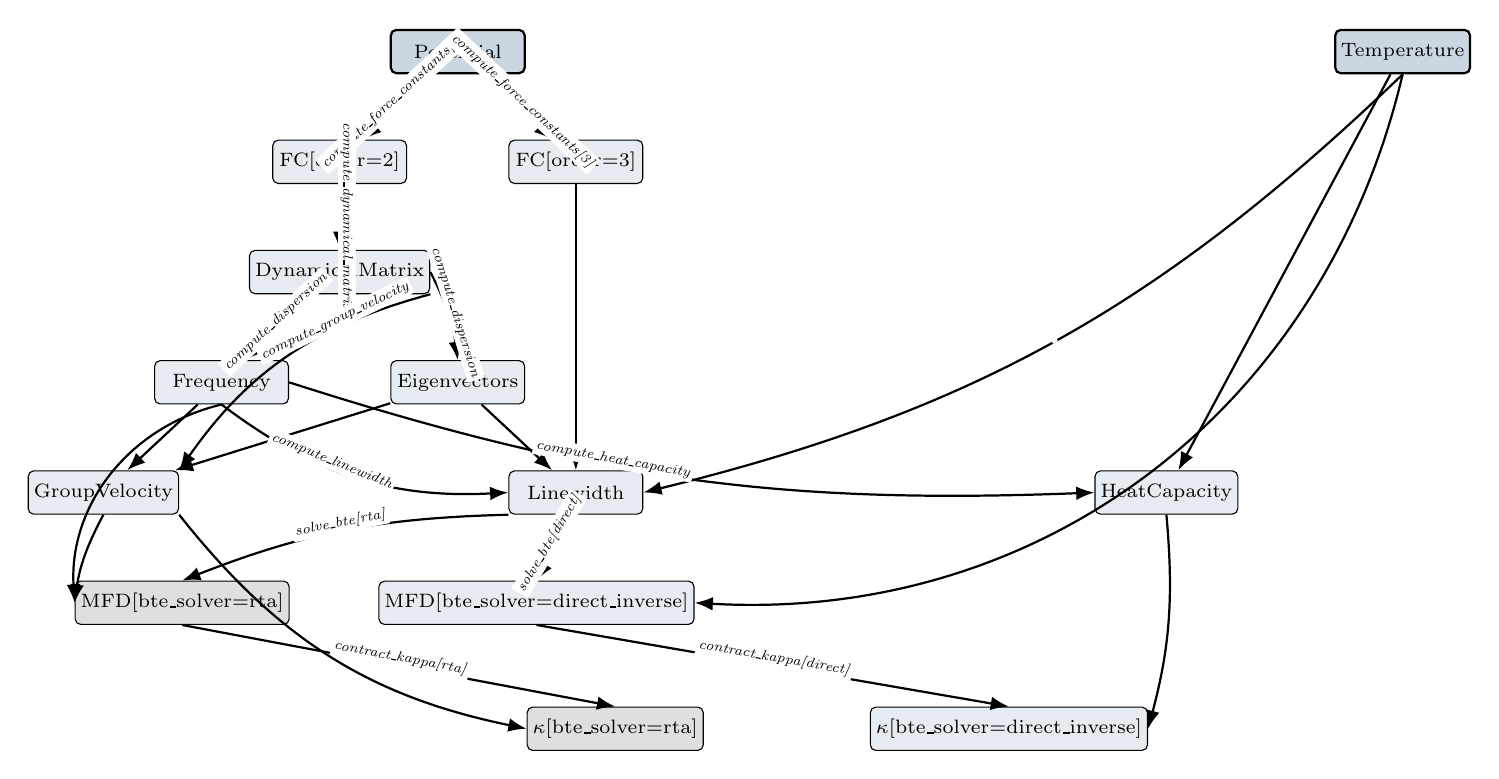
\begin{tikzpicture}[
  >=Latex,
  node distance=0.3cm,
  abstractnode/.style={draw, rounded corners=2pt, minimum width=1.7cm, minimum height=0.55cm,
                       font=\scriptsize, fill=abstrcol!12, inner sep=2pt},
  sourcenode/.style={draw, rounded corners=2pt, minimum width=1.7cm, minimum height=0.55cm,
                     font=\scriptsize, fill=abstrcol!25, inner sep=2pt, thick},
  stubedge/.style={->, thick, dashed},
  arr/.style={->, thick},
  oplabel/.style={font=\tiny\itshape, sloped, midway, above=-1pt, fill=white, inner sep=1pt},
]

% Source row
\node[sourcenode] (POT) at (0, 0) {Potential};
\node[sourcenode] (TMP) at (12, 0) {Temperature};

% FC row
\node[abstractnode] (FC2) at (-1.5, -1.4) {FC[order=2]};
\node[abstractnode] (FC3) at ( 1.5, -1.4) {FC[order=3]};

% Dynamical matrix
\node[abstractnode] (DM)  at (-1.5, -2.8) {DynamicalMatrix};

% Frequency / Eigenvectors
\node[abstractnode] (FRQ) at (-3, -4.2) {Frequency};
\node[abstractnode] (EIG) at ( 0, -4.2) {Eigenvectors};

% Mode-resolved
\node[abstractnode] (GV) at (-4.5, -5.6) {GroupVelocity};
\node[abstractnode] (HC) at ( 9, -5.6) {HeatCapacity};
\node[abstractnode] (LW) at ( 1.5, -5.6) {Linewidth};

% BTE - split by bte_solver
\node[abstractnode, fill=gray!25] (MFDR) at (-3.5, -7.0) {MFD[bte\_solver=rta]};
\node[abstractnode]               (MFDI) at ( 1.0, -7.0) {MFD[bte\_solver=direct\_inverse]};

% kappa - split by bte_solver
\node[abstractnode, fill=gray!25] (KAPR) at ( 2.0, -8.6) {$\kappa$[bte\_solver=rta]};
\node[abstractnode]               (KAPI) at ( 7.0, -8.6) {$\kappa$[bte\_solver=direct\_inverse]};

% --- arrows ---
\draw[stubedge] (POT) -- node[oplabel] {compute\_force\_constants[2]} (FC2);
\draw[stubedge] (POT) -- node[oplabel] {compute\_force\_constants[3]} (FC3);
\draw[arr] (FC2) -- node[oplabel] {compute\_dynamical\_matrix} (DM);
\draw[arr] (DM)  -- node[oplabel] {compute\_dispersion} (FRQ);
\draw[arr] (DM.east) to[bend left=10] node[oplabel] {compute\_dispersion} (EIG.north);
\draw[arr] (DM.south east) to[bend right=20] node[oplabel, pos=0.3] {compute\_group\_velocity} (GV.north east);
\draw[arr] (FRQ) -- (GV);
\draw[arr] (EIG) -- (GV);
\draw[arr] (FRQ.south) to[bend right=20] node[oplabel, pos=0.4] {compute\_linewidth} (LW.west);
\draw[arr] (EIG) -- (LW);
\draw[arr] (FC3) -- (LW);
\draw[arr] (TMP.south) to[bend left=15] node[oplabel] {} (LW.east);
\draw[arr] (FRQ.east) to[bend right=10] node[oplabel, pos=0.4] {compute\_heat\_capacity} (HC.west);
\draw[arr] (TMP) -- (HC);
% solve_bte to two MFDs
\draw[arr] (LW.south west) to[bend right=10] node[oplabel, pos=0.5] {solve\_bte[rta]} (MFDR.north);
\draw[arr] (LW.south) -- node[oplabel] {solve\_bte[direct]} (MFDI.north);
\draw[arr] (FRQ.south) to[bend right=40] (MFDR.west);
\draw[arr] (GV.south) to[bend right=10] (MFDR.west);
\draw[arr] (TMP.south) to[bend left=40] (MFDI.east);
% contract_kappa to two kappas
\draw[arr] (MFDR.south) -- node[oplabel] {contract\_kappa[rta]} (KAPR.north);
\draw[arr] (MFDI.south) -- node[oplabel] {contract\_kappa[direct]} (KAPI.north);
\draw[arr] (HC.south) to[bend left=10] (KAPI.east);
\draw[arr] (GV.south east) to[bend right=20] (KAPR.west);

\end{tikzpicture}%
}
\caption{Core $\kappa$ chain of the operator DAG for lattice thermal transport
(12 nodes / 14 edges shown; the full DAG has 54 nodes / 55 edges once the
derived-observable tier --- PhononDOS, Grüneisen, PhaseSpace, VolumetricHeatCapacity,
MolarHeatCapacity, the thermodynamic siblings (HelmholtzFreeEnergy, Entropy,
InternalEnergy and their molar contractions), the polar-correction inputs
(BareDynamicalMatrix, BornCharges, DielectricTensor), the per-channel
Linewidth split, the Wigner/QHGK transport variants, the cumulative-$\kappa$
distributions, the MD-primitive tier (Trajectory, HeatCurrent, HeatCurrentACF,
VelocityAutocorrelation, MeanSquaredDisplacement), and the three MD-based
$\kappa$ Pattern-A terminals (Green-Kubo, NEMD, HNEMD) --- is included; see
the interactive map at \texttt{docs/map/} for the live view). The
two darker top boxes (\texttt{Potential}, \texttt{Temperature}) are source nodes;
the dashed edges from \texttt{Potential} represent the stubbed Phase-1 upstream.
\texttt{MeanFreeDisplacement} and $\kappa$ split into two parameterized variants by
\texttt{bte\_solver}: the gray-shaded \texttt{[rta]} variants are HiddenSpaces
(RTA's $1/\Gamma$ non-linearity breaks gauge invariance), the unshaded
\texttt{[direct\_inverse]} variants are ObservableSpaces (the full LBTE preserves it).
Each derived edge carries a sympy formula; sources carry identity formulas. All
nodes are outputs of some operator; cross-code comparison happens at ObservableSpace
nodes (after the operator layer's spec-derived unit and normalization conversion). Other
HiddenSpaces (\texttt{Eigenvectors}, \texttt{GroupVelocity}, \texttt{Linewidth})
are not visually distinguished in this diagram but are gauge-dependent in the same
sense.}
\label{fig:dag}
\end{figure}

\subsection{Representation functors (codes)}

Each adapter is a representation functor over the operator DAG. Fifteen
adapter modules are now ingested in the thermal-transport domain alone (31
rails map the whole graph), in three tiers. The four BTE / harmonic codes that consume
force constants:

\begin{itemize}[leftmargin=2em]
  \item \textbf{kaldo} (Python). Computes harmonic and anharmonic phonon transport from
        force constants, supporting iterative BTE, RTA, and the Wigner formulation.
        Most intermediate states are exposed via Python attributes on the
        \texttt{Phonons} object. kaldo's \texttt{Conductivity(method='inverse')}
        realizes the canonical \texttt{bte\_solver=direct\_inverse}.
  \item \textbf{phono3py} (C/Python). Computes lattice thermal conductivity from
        third-order force constants. Intermediate quantities are exposed in HDF5
        outputs. \texttt{run\_thermal\_conductivity(is\_LBTE=True)} realizes the
        canonical \texttt{bte\_solver=direct\_inverse}.
  \item \textbf{phonopy} (C/Python). The harmonic-only sibling of phono3py:
        emits frequencies, group velocities, the DOS, the molar heat capacity,
        and (via \texttt{PhonopyGruneisen}) mode Grüneisen parameters from a
        finite-difference $\omega(V)$ rather than the canonical Maradudin--Fein
        closed form. No three-phonon scattering, so the adapter covers the
        harmonic half of the DAG only.
  \item \textbf{ShengBTE} (Fortran/MPI). Solves the full linearized BTE
        iteratively. The harmonic chain is delegated to phonopy/QE upstream;
        ShengBTE consumes FC2/FC3 files and writes
        \texttt{BTE.KappaTensorVsT\_\{RTA,CONV\}}, \texttt{BTE.\{omega, v, gruneisen,
        P3, dos\}}, etc. Per-mode heat capacity is not exposed (only
        \texttt{BTE.cv}), so the adapter targets \texttt{VolumetricHeatCapacity}
        rather than \texttt{HeatCapacity} on that branch.
\end{itemize}

\noindent and three phase-2 additions --- an ASE Potential anchor and two
molecular-dynamics codes that realise the MD-primitive tier and the MD-based
$\kappa$ paths:

\begin{itemize}[leftmargin=2em]
  \item \textbf{ase} (Python protocol). Not a thermal-transport code: it supplies
        only the shared \emph{Potential} / force-evaluation anchor
        (\texttt{provide\_potential} via \texttt{ase.Atoms.calc}). The four BTE
        codes above cite the \texttt{ase} adapter as their canonical Potential
        source, so a cross-code $\kappa$ comparison rests on one declared force
        field rather than an implicit shared assumption.
  \item \textbf{LAMMPS} (C++/Python). Classical molecular dynamics. Native
        \texttt{pair\_style} Potential, \texttt{Temperature} (global,
        region, and chunked-profile variants), plus the MD-primitive tier
        (\texttt{Trajectory}, \texttt{HeatCurrent}, \texttt{HeatCurrentACF},
        \texttt{VelocityAutocorrelation}, \texttt{MeanSquaredDisplacement} via
        \texttt{compute heat/flux}, \texttt{compute vacf}, \texttt{compute msd},
        \texttt{fix ave/correlate}) and the equilibrium Green-Kubo and
        Müller-Plathe NEMD $\kappa$ paths. HNEMD is recorded as not-exposed
        (it routes through GPUMD).
  \item \textbf{GPUMD} (CUDA/C++). GPU-accelerated classical MD specialised for
        thermal transport. NEP-potential (neuro-evolution) anchor, the same
        MD-primitive tier, and the Green-Kubo (\texttt{compute\_hac}) and
        HNEMD (\texttt{compute\_hnemd}) $\kappa$ paths --- HNEMD being GPUMD's
        signature method; direct NEMD is recorded as not-exposed (routes
        through LAMMPS).
\end{itemize}

\noindent and one source-tier addition grounding the upstream the BTE codes
consume as given:

\begin{itemize}[leftmargin=2em]
  \item \textbf{Quantum ESPRESSO} (Fortran/MPI). First-principles DFT and
        DFPT. Grounds the source tier: \texttt{ForceConstants[order=2]}
        (\texttt{q2r.x} real-space constants in Ry/bohr$^2$),
        \texttt{BornCharges} and \texttt{DielectricTensor} (\texttt{ph.x}
        linear response, turning the \texttt{provide\_*} sources into
        computed quantities), \texttt{BareDynamicalMatrix} /
        \texttt{DynamicalMatrix} (raw un-mass-weighted $C(\mathbf{q})$
        files; mass weighting applied only at diagonalization),
        \texttt{Frequency} (linear cm$^{-1}$ / THz), \texttt{Eigenvectors},
        and \texttt{PhononDOS} via \texttt{matdyn.x}. The adapter records
        the DFPT method (versus finite displacements), QE's internal
        space-group machinery, and the Gonze NAC scheme; derived from the
        anchored scan catalog \texttt{scans/qe-phonon.json}.
\end{itemize}

Each adapter spec declares per-space units, normalization overrides, and notes
(\texttt{SpaceRepresentationSpec}), plus per-operator parameter units, scheme
overrides, and discretization choices (\texttt{OperatorRepresentationSpec}). Differences
from the operator layer's canonical declarations surface as conversion factors at
spec-load time.

\subsection{Verification on silicon (Tersoff potential)}
\label{ssec:silicon-verification}

The operator layer's predictions have been verified end-to-end against numerical
runs of kaldo and phono3py on silicon at the Tersoff potential, $8\times 8\times 8$
q-mesh, $T = 300\,\text{K}$, broadening stdev $0.1\,\text{THz}$:

\begin{center}
\begin{tabular}{lll}
\toprule
ObservableSpace / contraction & Operator prediction & Empirical residual \\
\midrule
\texttt{Frequency} per-mode (\textbf{O})            & factor $1$ (both linear THz)  & $5\times 10^{-4}$ \\
\texttt{HeatCapacity} per-mode (\textbf{O})         & factor $1/e \approx 6\times 10^{18}$ & $3\times 10^{-5}$ \\
$\sum_{q\nu}\Gamma$ contracted (\textbf{O})          & factor $1/(4\pi)$              & $5\times 10^{-4}$ \\
$\kappa$\texttt{[bte\_solver=direct\_inverse]} (\textbf{O})\footnotemark{} & factor $1$                & $4\times 10^{-3}$ \\
\midrule
\texttt{Linewidth} per-mode (\textbf{H})            & \textsc{Not\_Comparable} & 25\% (diagnostic only) \\
$\kappa$\texttt{[bte\_solver=rta]} (\textbf{H})     & \textsc{Not\_Comparable} & 4\% (diagnostic only) \\
\bottomrule
\end{tabular}
\end{center}
\footnotetext{This $0.4\%$ residual and the $\sim 10\%$ figure that the map's
published instances and the end-to-end cross-code experiments
(\texttt{experiments/silicon\_tersoff}, the sigma sweep) show for kaldo versus
phono3py at $8\times 8\times 8$ with independently computed force constants are not
in contradiction: they describe different comparisons. The $\sim 10\%$ number is
what two codes give when each computes its own force constants; the $0.4\%$ figure
comes from a more controlled comparison whose exact setup is being re-established.
Until that setup is re-pinned, treat the two numbers as measuring different things.}

All ObservableSpace comparisons pass at $\le 1\%$ tolerance; all HiddenSpace per-element
comparisons return \textsc{Not\_Comparable}. The $1/(4\pi)$ factor on $\Gamma$
decomposes into a $1/(2\pi)$ \emph{unit} factor (kaldo angular vs phono3py linear
THz) and a $1/2$ \emph{normalization} factor (kaldo $\Gamma = 2\,\text{Im}\,\Sigma$
$\Rightarrow$ \texttt{linewidth\_2x\_imag\_self\_energy} with
\texttt{to\_operator}~$=0.5$; phono3py uses the canonical normalization). Both
factors were derived by the operator layer from declared adapter specs, then
applied mechanically to the diagnostic data.

The 4\% disagreement on $\kappa_\text{RTA}$ is the operator layer's structural prediction
working as designed: RTA's approximation breaks $\kappa$'s gauge invariance via the
$1/\Gamma$ non-linearity, so the per-mode Linewidth redistribution propagates into
$\kappa$. Typing $\kappa_\text{RTA}$ as a HiddenSpace makes this a non-anomaly; the
gauge-invariant $\kappa_\text{LBTE}$ agrees to 0.4\%.

\paragraph{Cross-paradigm $\kappa$ (phase 2 P4).} On the same Si-Tersoff
worked example, the LAMMPS Green-Kubo path
(\texttt{contract\_kappa[transport\_model=green\_kubo]} reached through the
P2 MD-primitive tier and the P3 contraction edge) returns a $\kappa$ value
that, in the small ensemble of equilibrium-MD runs the framework drives,
is expected to land within $\sim 20$--$30\%$ of $\kappa_\text{LBTE}$. That tolerance is
Green-Kubo's empirical signal-to-noise floor on a few-hundred-atom
supercell, not a framework concern. The driver at
\texttt{experiments/silicon\_tersoff/run\_lammps\_gk.py} generates the input
script and the supercell data file regardless of whether \texttt{lmp} is on
\texttt{PATH}; the \texttt{spec\_demo.py} cross-paradigm audit section and
the corresponding \texttt{test\_silicon\_consolidation.py} smoke test
gracefully skip when the resulting \texttt{kappa\_lammps\_gk.npy} is
absent. The NEMD and HNEMD analogues land in P5 and P6.

\subsection{Phase 1 scientific capabilities}

Phase 1 yields two immediate scientific capabilities, each of which is an artifact the field does
not currently produce. A third capability is the long-term goal toward which the operator layer is
oriented but is deferred to Phase 2.

\begin{itemize}[leftmargin=2em]
  \item \textbf{Cross-code reconciliation at canonical intermediate states.} When kaldo and
        ShengBTE disagree on a final $\kappa$, the operator layer localizes the divergence to the
        first operator state at which the representations stop agreeing, and attributes it to a
        specific operation along the provenance. This is a structural diagnosis: the framework
        identifies where two codes do something different, regardless of the magnitude of the
        difference.
  \item \textbf{A unified framework for theory-experiment comparison.} The same operator DAG
        accepts experimental measurements as additional evidence on the same nodes,
        with the same alignment machinery as for cross-code comparison. The two
        Glassbrenner--Slack 1964 steady-state thermal conductivities of bulk
        single-crystal silicon and germanium (Part~\ref{part:status}) are the map's
        first measurement instances, sitting on the same $\kappa$ node as the
        computed values.
  \item \textbf{An agreement layer over the committed values.} The map already holds
        same-conditions comparisons, and a derived agreement view
        (\texttt{docs/data/agreement.json}, the \texttt{/agreement/} page) surfaces
        them as honest reporting of what the data contains. It groups the committed
        instances that name the same base observable, the same material, and the
        same physical conditions, differing only in the method or the code that
        produced them, and reports each group's spread. The concrete cross-code
        case is silicon at the Tersoff potential, $8\times 8\times 8$ mesh,
        $T=300\,\text{K}$: kaldo and phono3py agree on direct inversion at $26.9$
        versus $24.3$ and on RTA at $19.5$ versus $16.7$ (in W/m~K), the same run
        both cross-method and cross-code; the silicon DFPT LDA case, $19\times
        19\times 19$ q-grid, quantum statistics, contrasts direct inversion at
        $147$ against RTA at $140$. The honesty caveat is the equivalence rule
        itself: two values are compared only when their base quantity, material,
        and every physical condition match and they differ solely in estimator,
        so a spread is a real method or code disagreement, never an
        apples-to-oranges artifact (the source paper is not a physical condition,
        so two solvers from one paper compare, and two codes on the same inputs
        are the strongest comparison).
\end{itemize}

\noindent\textbf{Deferred to Phase 2:}
\begin{itemize}[leftmargin=2em]
  \item \textbf{Decomposed error bounds on $\kappa$.} The operator layer is designed to eventually
        produce the central value of $\kappa$ together with an operator decomposition of its
        total error into the truncation error of the perturbation series and the discretization
        error of the chosen mesh. The architecture supports this; the implementation of the
        composition algebra is a research problem reserved for Phase 2.
\end{itemize}

\section{Implementation layout}
\label{sec:layout}

The Python package \texttt{omai} factors into two top-level sub-packages
plus one per domain:

\begin{itemize}[leftmargin=2em, itemsep=0.3em]
  \item \texttt{omai.operator} --- operator layer machinery for the operator world.
        \texttt{Space} (base class), \texttt{ObservableSpace} and \texttt{HiddenSpace}
        (subclasses, with gauge-discipline fields on the latter), \texttt{Field},
        \texttt{Operator}, \texttt{Parameter}, \texttt{Dimension},
        \texttt{topological\_order},
        \texttt{validate\_dag} (Level 1 discipline enforcement), and
        \texttt{GaugeAction} / \texttt{check\_invariance} (Level 2 operator
        gauge proofs). Code-agnostic and domain-agnostic.
  \item \texttt{omai.representation} --- the bridge.
    \begin{itemize}[leftmargin=1.2em]
      \item \texttt{units.py}: the \texttt{Unit} class, named unit instances, strict
            same-dimension \texttt{conversion\_factor}.
      \item \texttt{normalizations.py}: the \texttt{Normalization} registry
            mirroring \texttt{units.UNITS} in shape --- each entry carries a
            \texttt{to\_operator} multiplier into canonical definitional form
            (e.g.\ \texttt{linewidth\_2x\_imag\_self\_energy} with factor
            $0.5$, \texttt{eV\_per\_A2\_per\_nm} with factor $10$).
      \item \texttt{adapter.py}: \texttt{SpaceRepresentationSpec} and
            \texttt{OperatorRepresentationSpec}; the two primitives
            \texttt{representation\_to\_operator} and
            \texttt{operator\_to\_representation} (each defined as the
            composition \texttt{unit.to\_operator}~$\cdot$~\texttt{normalization.to\_operator});
            and the diagnostic helpers
            \texttt{representation\_scheme\_match} and
            \texttt{representation\_discretization\_match}.
      \item \texttt{instance.py}: the \texttt{Representation} runtime data class
            and \texttt{represent()} constructor.
      \item \texttt{compare.py}: numerical and structural comparison APIs.
            \texttt{to\_operator(m)} canonicalises a representation into operator
            form; \texttt{to\_representation(m\_op, target\_spec)} is the
            inverse. \texttt{compare\_operators(spec\_a, spec\_b)} returns an
            \texttt{OperatorComparisonResult} (categorical: do the two adapter
            specs describe the same operator?). \texttt{compare\_representations}
            (aliased as \texttt{compare}) returns a
            \texttt{RepresentationComparisonResult} with the five-status
            verdict and residuals.
    \end{itemize}
    Code-agnostic.
  \item \texttt{omai.thermal\_transport} --- the lattice-thermal-transport domain.
    \begin{itemize}[leftmargin=1.2em]
      \item \texttt{operator/nodes.py}: the domain's 54 spaces as \texttt{ObservableSpace} or
            \texttt{HiddenSpace} instances with their fields.
      \item \texttt{operator/edges.py}: the domain's 55 operators with sympy formulas
            and \texttt{auxiliary\_formulas} (the \texttt{compute\_linewidth}
            $|V_3|^2$ kernel and the \texttt{solve\_bte[direct\_inverse]}
            collision matrix $M$); sympy symbols and \texttt{IndexedBase}
            declarations.
      \item \texttt{operator/gauges.py}: concrete \texttt{GaugeAction}
            instances for the domain (e.g.\ U(1) phase on Eigenvectors).
            Mechanically verifies operator formulas are gauge-invariant.
      \item \texttt{representation/kaldo.py},
            \texttt{representation/phono3py.py},
            \texttt{representation/phonopy.py},
            \texttt{representation/shengbte.py},
            \texttt{representation/qe.py},
            \texttt{representation/ase.py},
            \texttt{representation/lammps.py},
            \texttt{representation/gpumd.py}: per-code adapter specs
            (one file per code), declaring units, normalizations, schemes,
            and discretization choices. Every operator in scope for a code
            now carries an \texttt{OperatorRepresentationSpec}; trivial source /
            contraction ops carry no schemes but exist to mark coverage
            on the map. Coverage renders on the site map (\texttt{docs/map/},
            generated data in \texttt{docs/data/}); the standalone per-code
            pipeline page was retired 2026-07-08 as redundant with the map's
            code rails. Per-operator scheme and discretization detail lives in
            the representation modules and this document; surfacing it in the
            map's edge panel is an open enhancement.
    \end{itemize}
\end{itemize}

\noindent The split mirrors the operator layer's architectural commitment: \texttt{omai.operator}
is the operator world; \texttt{omai.representation} is the bridge to the numeric world;
\texttt{thermal\_transport} is the first domain instantiated against them. Further
domains follow the same pattern in their own folder (electronic transport has
since landed exactly this way); no change to the operator-level packages is
required to add one.

\section{Open Questions and Deferred Decisions}
\label{sec:open}

We list the architectural questions that remain open and the principled grounds on which they
were deferred.

\subsection{Algebra of error composition (deferred to Phase 2)}

The operator layer is designed to carry error formulas as operator expressions, but Phase 1 does not
implement the algebra by which they compose. Composing two errors in independent small parameters
($O(\lambda^4) + O(N^{-2})$) is well-defined; composing two errors in the same parameter requires
care; composing constant-offset errors (e.g., basis-set incompleteness) with asymptotic ones is
yet another case. The right algebra is itself a research subproblem and will be developed
alongside concrete worked examples in Phase 2. The Phase 1 type system reserves the slots
required for error formulas (operation metadata, discretization error model, representation
total error) but populates them with placeholders rather than computed compositions.

\subsection{When to lift to Lean}

We have committed to keeping the operator layer Lean-compatible without being Lean-dependent. The
question of when (and whether) to actually project the operator layer into Lean is deferred until
the Python prototype has stabilized. A reasonable trigger for this decision is the moment at
which we have enough concrete examples that designing Lean types in isolation becomes
counterproductive.

\paragraph{T3-evolve as a pre-Lean realisation.} The sympy chain composer
(\texttt{omai.operator.compose.compose\_path}) is the in-sympy realisation of the
Lean commitment in this subsection. Given a path of explicit-equation edges in the
operator DAG, it substitutes each edge's RHS into the next, producing a composed
symbolic expression at the path's terminal node. Implicit-equation edges (e.g.,
\texttt{solve\_bte\_*}) raise \texttt{ImplicitEdgeBoundary} with the partial
expression attached --- they mark the open research subproblem of composing across
an implicit BTE solve, which is the natural next step toward a full Lean
projection. The composer's existence is evidence that the operator-layer formulas
are not merely documentation: they are mechanically composable today, and the same
substitution machinery transliterates to a Lean tactic when the projection is
eventually performed.

\subsection{Provenance equivalence}

The implemented kernel replaces provenance-based identity with content identity
(Part~\ref{part:kernel}): two states with the same content are the same state
regardless of history, and adding an alternative producing route never re-mints a
node. What remains genuinely open is the \emph{edge}-level version of this
question. Because an edge id includes its formula fingerprint, a factored and an
expanded form of the same physics mint different edge ids and coexist as parallel
producing edges. When the two are provably equivalent (e.g., Fourier transform of
a real symmetric matrix and direct frequency-domain assembly yielding the same
\texttt{Dispersion}), an explicit, reviewer-approved \texttt{equate} record in the
log ties them together at the edge level. That record now exists in the store
(Part~\ref{part:kernel}); the general equivalence calculus, deciding which such
equivalences hold by proof rather than by curation, is still deferred because we
want concrete examples before designing it.

\subsection{Sprint 1 scope}

The first concrete deliverable is a Python implementation. We have considered three scopes:

\begin{enumerate}[leftmargin=2em]
  \item \emph{Narrowest:} kaldo only, harmonic sub-DAG (force constants $\to$ dynamical matrix
        $\to$ dispersion). 4--5 states, fastest to ship.
  \item \emph{Recommended:} kaldo only, full thermal-conductivity DAG. 10--15 states, end-to-end
        on silicon. The operator layer skeleton plus one full adapter.
  \item \emph{Broader:} kaldo plus phono3py, full DAG. Validates the cross-code story earlier but
        adds adapter work in parallel with framework design.
\end{enumerate}

The recommended scope (option 2) is the smallest scope that is still a credible proof of concept
of the framework, and the choice of one adapter (kaldo) lets us validate the operator layer design
before generalizing. Sprint 2 adds phono3py and ShengBTE adapters, at which point the cross-code
demo of \S\ref{sec:demo} becomes real. \emph{Status as of 2026-05}: the
recommended scope shipped; Sprint 2 also shipped, with phono3py, phonopy,
and ShengBTE all ingested and the cross-code Si silicon comparison
(\texttt{experiments/silicon\_shengbte/}) demonstrating $\kappa_\text{RTA}$
agreement to $\le 8\%$ across the three transport codes after the operator
layer's spec-derived conversions.

\subsection{Implementation language}

We have committed to Python for Sprint 1. The trade-offs were:

\begin{itemize}[leftmargin=2em]
  \item \textbf{Python (chosen).} All target codes have Python bindings or wrappable interfaces.
        The Python type system, augmented with \texttt{pydantic} or \texttt{attrs} and runtime
        checks, is sufficient for the operator layer's first-cut type discipline. The development
        speed is dominant, since adapter work is the bulk of the time cost.
  \item \emph{Typed compiled language (Rust, OCaml, TypeScript).} Stronger type guarantees from
        the start. Rejected for Sprint 1 because the foreign-function interface to existing
        Python codes adds friction proportional to the operator layer's surface, and we want
        framework iteration to be cheap.
  \item \emph{Lean.} Not the right tool for running scientific computations;
        reserved as a verification target, a reservation since cashed in: the
        verified layer of Part~\ref{part:status} compiles today.
\end{itemize}

\section{Outlook}
\label{sec:outlook}

The operator layer is an architectural commitment, not an implementation. The implementation
began as a Python skeleton plus adapters for three thermal-transport codes and has since grown
to the 31-rail map of Part~\ref{part:status}. The
artifact that motivates the project---a paper-worthy demonstration of cross-code reconciliation
and decomposed error bounds for lattice thermal conductivity---is downstream of the operator layer but
is the operator layer's first proof-of-value.

The project's stewardship follows its architecture (2026-07-12). The map, its
evidence, and the rules that govern changes are the commons, held by
OpenMaterials-AI, an open initiative structured as a foundation in formation:
map data is licensed CC BY 4.0, the kernel Apache 2.0, and the governance
document states the boundary rule plainly: the commons owns the ledger and its
laws; companies own tools and products built on top. The interfaces and the AI
improvement engine are built by Da Vinci Labs against that boundary. The same
document states data ownership and fairness (2026-07-13): evidence stays its
owner's (contribution grants a non-exclusive CC~BY~4.0 license, never a
transfer, with no copyright assignment and no CLA), raw simulation and
experimental artifacts are never ingested, and attribution is enforced in both
directions, upstream through code rails and page-anchored quotes as a merge
gate, downstream through the map version's provenance.

Four longer-term directions follow naturally from the design:

\begin{itemize}[leftmargin=2em]
  \item \textbf{Verification.} Project the operator layer into Lean, allowing
        approximation theorems to be formally proved rather than asserted. The
        provenance mechanism makes this projection well-defined: each operation in $\pi$
        corresponds to a Lean lemma whose statement is the operation's error formula.
        The first tiers are built, verified, and CI-gated (2026-07-17): \texttt{lean/}
        is a standalone lake package on Lean~4.31.0 depending on physlib, the
        community Lean~4 physics library, pinned by revision. Tier~1 declares every
        exported node as a physics \texttt{Dimension} and proves one theorem per
        verified executable edge: 89 nodes and 12 edge theorems compile against
        physlib's five bases, and a generated seven-base extension adds the
        amount-of-substance, current, and luminous-intensity quantities, so 106 of
        the map's 114 nodes carry a machine-checked dimension. Of the eight left
        out, five (\texttt{Structure}, \texttt{Potential}, and the opaque
        autocorrelation kinds) have no dimensional content to prove; three
        (\texttt{CellVolume}, \texttt{AtomicMass}, \texttt{AtomCount}) have
        dimensions the exporter does not yet walk, generator work, not proof
        work. Tier~2
        states the map's executable identities as real-valued theorems against
        Mathlib, 13 in all: composition theorems that substitute an upstream identity
        into a downstream one and prove the chained form equals the flat form, and
        law theorems for standalone rational operators; a units file anchors the
        map's SI convention. A CI gate recompiles the full proof on every pull
        request that touches the map or the generators, with warnings promoted to
        errors, so the verified badge is the live state of the claim. A public
        formalization roadmap rates all 114 operators by what a proof of the formula
        would take (12 rational identities closed by the generator, 44 needing real
        analysis, 18 trivially reflexive, 40 opaque code outputs with nothing
        algebraic to prove), and a hand-reviewed crosswalk links map nodes to the
        physlib declarations that formalize the same concepts. The
        approximation-error theorems remain future work.
  \item \textbf{Theory-experiment integration.} Extend the representation functor to ingest
        experimental observables. The operator layer's graph-alignment machinery applies uniformly,
        so a measured $\kappa$ becomes another representation of the abstract $\kappa$, and
        ``does the theory match experiment'' becomes graph-alignment with one functor being
        empirical.
  \item \textbf{Grounded LLM agents.} An LLM operating over typed operator states (rather than
        text tokens) constructs workflows by emitting operator operations. The framework
        type-checks each emission, eliminating the drift problem that plagues current
        text-token agents. The action space is finite, typed, and physically meaningful.
  \item \textbf{Learned shortcuts.} The kernel already types ML surrogates as
        declared, non-authoritative shortcuts of exact-edge paths
        (\texttt{LearnedOperator}, 2026-07-13): the shortcut names its path, inherits
        its schemes, cites its model artifact and training labels, and stays
        permanently subordinate to the exact edges and the evidence. The first map
        declaration ships when a released model artifact and its evidence instances
        land together; the natural candidate is the three-phonon linewidth surrogate
        that amortizes \texttt{ForceConstants[order=3]} into weights.
\end{itemize}

The unifying claim of the design is that scientific computing has been organized around the
wrong atomic unit. The instruction-in-an-input-file unit is too low; the natural-language
description is too high; the equation-in-a-paper unit is too disconnected from execution. The
right unit, at least for materials science, is the operator operation between typed physics
states. Once that commitment is made, much of the rest of the architecture writes itself.

% =====================================================================
\part{The Kernel}
\label{part:kernel}
% =====================================================================

\noindent
The architecture of Part~\ref{part:architecture} is a design; this part records
what was built. The kernel is the protocol core of Part~\ref{part:product} made
real, first on the 51-node genesis map and since grown through its gates to
today's map (Part~\ref{part:status}): composable dimensions with a dimensional
gate, content identity by hashing, a log-first versioned store with a
tamper-evident hash chain, a frozen genesis, and the source index. After the
kernel landed, the
map's source of truth is data, an append-only log plus a materialized view; the
Python operator layer became an authoring client that emits change records; and
every future scan-derived contribution (Quantum ESPRESSO's DFT ground state,
LAMMPS, the remaining materials skills) enters through validation gates rather
than hand-edited Python.

The kernel was built before bulk growth from code scans, and deliberately so.
Identity hashes include a node's dimension, gauge class, and index signature. Had
those changed representation later, for instance flat dimension tags becoming
composable exponent vectors, every hash in the map would re-mint on day one of
the protocol. The map was small enough at genesis (then tens of nodes) to
verify the genesis migration by hand; after the code scans it would not
be.

\section{Dimension algebra and the dimensional gate}
\label{sec:kernel-dimensions}

Dimensions enter the identity hash, so they were made composable first. The flat
\texttt{Dimension("thermal\_conductivity")} tags were replaced with exponent
vectors over the seven SI base dimensions ($M$, $L$, $T$, $\Theta$, $N$, $I$,
$J$), with an \texttt{opaque} escape hatch (\texttt{exponents = None}) for
deliberately unmodeled internals: the \texttt{Potential}, \texttt{Structure},
\texttt{Trajectory} fields, and the autocorrelation kinds that were typed opaque.
\begin{quote}
\texttt{Dimension(name, exponents: tuple[Fraction, ...] | None)}\quad\emph{(None = opaque)}
\end{quote}
Multiplication, division, and integer powers are defined on dimensions; equality
compares exponents, and opaque dimensions compare by name. Every existing named
constant kept its name and all of its call sites ($\mathtt{ENERGY} = M\cdot
L^2\cdot T^{-2}$, $\mathtt{THERMAL\_CONDUCTIVITY} = M\cdot L\cdot T^{-3}\cdot
\Theta^{-1}$, and the rest), so the change was zero churn outside
\texttt{dimensions.py}. The algebra preserves and extends \texttt{dimension\_si\_scale}
compositionally: a derived dimension's SI scale is the product of its factors'
scales, which the executor's monomial-contraction rescaling (Part~\ref{part:architecture})
depends on.

On top of the algebra sits a new validation gate. For closed-form \texttt{Eq}
edges, the gate checks dimensional consistency of the left-hand side against the
right-hand side wherever every symbol's dimension is known, drawn from the
per-space fields and the edge parameters. This is the mechanical form of
Part~\ref{part:product}'s first validation rule (``dimensional agreement on every
edge''), and it is the cheapest strong filter for everything the parsers will
later propose. The gate partitions every closed-form \texttt{Eq} edge into
\emph{ok}, \emph{documented-schematic violation}, or \emph{skipped} (a formula the
gate cannot check: an implicit solve, a procedural fit); the live tally is in
Part~\ref{part:status}. The only two violations are
\texttt{compute\_gruneisen} and \texttt{compute\_phase\_space\_3phonon}, kept
deliberately schematic (see \S\ref{sec:kernel-normalization}).

\section{Content identity}
\label{sec:kernel-identity}

Names and symbols are metadata, never identity. Hashes are \texttt{sha256} over
canonical JSON (sorted keys, no whitespace); the store keeps full digests and
displays a 12-hex prefix.

\paragraph{Node id.} A node's id is
\[
  \mathrm{H}(\text{quantity\_tag},\ \text{field\_signatures},\ \text{gauge\_class},\ \mathrm{sorted}(\text{labels})),
\]
where each ingredient is:
\begin{itemize}[leftmargin=2em, itemsep=0.2em]
  \item \textbf{quantity\_tag} is a curated identifier (\texttt{entropy},
        \texttt{heat\_capacity}, \texttt{potential}, \texttt{structure},
        \texttt{dynamical\_matrix}, \texttt{bare\_dynamical\_matrix}, \ldots) from
        a controlled, versioned registry in core, exactly like labels and index
        kinds. It is the semantic distinction the structural fields cannot carry.
  \item \textbf{field\_signatures} is the sorted multiset of
        (\texttt{dimension\_canonical}, \texttt{index\_kind\_signature}) over
        \emph{all} of the space's fields (\texttt{Trajectory} has two), not a
        single dimension. The \texttt{index\_kind\_signature} is the tuple of
        index \emph{kinds} drawn from a small controlled registry
        (\texttt{atom}, \texttt{cartesian}, \texttt{qpoint}, \texttt{branch},
        \texttt{lattice\_vector}, \texttt{timestep}, \texttt{lag},
        \texttt{omega\_bin}, \texttt{mfp\_bin}, \ldots); kinds carry the
        gauge and symmetry semantics Part~\ref{part:product} assigns to indices.
  \item \textbf{gauge\_class} is \texttt{observable} for an observable node,
        \texttt{parameter} for a promoted parameter, or the string
        \texttt{hidden/<kind>/<gauge\_group>} for a hidden node, where
        \texttt{kind} is \texttt{scaffolding} or \texttt{approximation} and
        \texttt{gauge\_group} is a registered ascii identifier.
  \item \textbf{labels} are the semantic type parameters
        (\texttt{bte\_solver=direct\_inverse}, \texttt{transport\_model=wigner},
        \texttt{channel=isotope}, \texttt{order=2}). Label keys and values live in
        a controlled, versioned registry, never free-form strings.
\end{itemize}
The production route is not part of the node id: Pattern~C nodes (a shared output
with alternative producing edges) keep one stable id, and adding a producer never
re-mints. \texttt{tier} and names, symbols, and descriptions are presentation
metadata, never identity. Promoted parameters (\texttt{CellVolume},
\texttt{AtomicMass}, \texttt{AtomCount}) receive quantity tags and dimensions like
any node.

\paragraph{The collision rationale: why the quantity tag.} An earlier candidate
made identity purely type-content, hashing only the field signatures, gauge
class, and labels with no curated tag. It was stress-tested against the live map
and \emph{false-merged seven real pairs of distinct quantities}, because physics
is full of same-typed distinct quantities:
\begin{itemize}[leftmargin=2em, itemsep=0.15em]
  \item \texttt{Entropy} $=$ \texttt{HeatCapacity} (same dimension, indices, gauge);
  \item \texttt{HelmholtzFreeEnergy} $=$ \texttt{InternalEnergy}, and their two
        \texttt{Molar*} counterparts (two more pairs);
  \item \texttt{Potential} $=$ \texttt{Structure} (both opaque source leaves);
  \item \texttt{BareDynamicalMatrix} $=$ \texttt{DynamicalMatrix};
  \item \texttt{Gruneisen} $=$ \texttt{PhaseSpace3Phonon}.
\end{itemize}
Seven false merges is disqualifying, so the semantic distinction is carried by a
curated \texttt{quantity\_tag} from the registry, and convergence becomes
registry-mediated: two contributors converge by mapping to the same registered
quantity, and the structural fields are validated against the tag (a wrong
dimension for a claimed quantity fails validation). This softens
Part~\ref{part:product}'s ``converge automatically'' wording: convergence is
through the shared registries, not by structural coincidence.

The consequence to hold onto is that \emph{labels carry the disambiguation work}.
Same-typed variants that must stay distinct
(\texttt{wigner\_populations} vs \texttt{wigner\_coherences} vs \texttt{wigner};
cumulative $\kappa$ with respect to $\omega$ vs with respect to mean free path)
are distinct only because of their labels, which is why label keys and values are
part of the protocol registry. A contribution using an unregistered label key
fails validation. Two parallel derivations of the same-typed unlabeled quantity
(for example a second producer of $\kappa$) converge onto one node with two
producing edges, which is the intended reconciliation-at-observables behavior, not
a false merge: the distinct physics stays on the edges, whose formula fingerprints
differ. The gauge class already separates RTA-style approximations from
observables without any label.

\paragraph{Edge id.} An edge's id is
\[
  \mathrm{H}(\text{output node id},\ \text{unordered set of input node ids},\ \text{formula\_fingerprint},\ \mathrm{sorted}(\text{schemes})).
\]
The \texttt{formula\_fingerprint} is the normalized \texttt{sympy.srepr} of the
formula. Sympy's canonical \texttt{Add}/\texttt{Mul} ordering already collapses
$c\,v^2\,\tau$ and $\tau\,v^2\,c$ to one tree; operators whose formula is a LaTeX
string fingerprint the string after whitespace normalization. Editing a formula
re-mints the edge and writes a supersede record. This is strict but honest: ``every
edge carries its formula'' is the product's core claim, so a different formula is a
different edge. Two points follow. First, the operator \emph{name} is not in the
hash: names are metadata (edited via \texttt{edit\_meta}), and identity is
structural, which matches Part~\ref{part:architecture}'s ``operation identity is
parameterized'' once ``parameters affecting physics'' is read as schemes, which
are in the hash. Second, the fingerprint canonicalizes commutative reordering but
\emph{not} general algebraic equivalence: a factored and an expanded form of the
same physics mint different edge ids, coexist as parallel producing edges, and are
reconciled only by an explicit, reviewer-approved \texttt{equate} record in the
log. That record realizes, at the edge level, the ``provenance equivalence''
mechanism Part~\ref{part:architecture} defers; it is a curation action, never
automatic. Approximation-error formulas (Part~\ref{part:architecture}'s Phase-2
slots on operations) are metadata, not identity: attaching or refining an error
formula later must not re-mint an edge.

\paragraph{Version hash.} The version hash chains the log,
$\mathrm{H}(\text{previous version hash} \parallel \text{canonical(change record)})$,
the tamper-evident chain from Part~\ref{part:product}, unchanged. The consequences
kept from Part~\ref{part:product} are structural convergence (same physics, same
hash), parallel routes for genuinely different decompositions, and the Merkle
ripple on foundational edits, handled by supersede records.

\section{The protocol registries}
\label{sec:kernel-registries}

Every string that enters a hash lives in a controlled, versioned registry in
core, so that a \texttt{qpoint} means the same kind in every domain and
cross-domain convergence is well-defined. There are four such registries:
\begin{enumerate}[leftmargin=2em, itemsep=0.2em]
  \item \textbf{Quantity tags} (\S\ref{sec:kernel-identity}): the curated
        per-quantity identifiers.
  \item \textbf{Index kinds}: one global registry of about twelve kinds
        (\texttt{atom}, \texttt{cartesian}, \texttt{qpoint}, \texttt{branch},
        \texttt{lattice\_vector}, \texttt{timestep}, \texttt{lag},
        \texttt{omega\_bin}, \texttt{mfp\_bin}, \ldots). Index kinds enter node
        identity and cross-domain convergence depends on them, so the registry is
        shared, not per-domain.
  \item \textbf{Label keys and values}: \texttt{bte\_solver},
        \texttt{transport\_model}, \texttt{channel}, \texttt{order}, \texttt{wrt},
        and their permitted values.
  \item \textbf{Gauge-group names}: the named gauge equivalences on hidden spaces,
        normalized to ascii identifiers before they enter any hash.
\end{enumerate}
A contribution referencing an unregistered tag, index kind, label key, or gauge
group fails validation. Registering a new one is a deliberate, versioned protocol
change.

\section{The log-first store}
\label{sec:kernel-store}

The versioned artifact lives in \texttt{map/} at the repository root, a peer of
\texttt{omai/} and \texttt{docs/} rather than a view inside the docs site, because
it is the protocol artifact anyone can fork and it stands on its own.

\paragraph{Record shapes.} \texttt{map/log.jsonl} is the append-only change log,
one canonical-JSON line per record with the shape
\[
  \{\texttt{seq},\ \texttt{op},\ \texttt{payload},\ \texttt{author},\ \texttt{date},\ \texttt{reason},\ \texttt{prev},\ \texttt{version}\},
\]
where \texttt{op} is one of \texttt{add\_node}, \texttt{add\_edge},
\texttt{edit\_meta}, \texttt{deprecate}, \texttt{supersede}, \texttt{equate}. The
\texttt{edit\_meta} op covers names, symbols, and descriptions, the non-identity
content that must be editable without re-minting; \texttt{supersede} ties an old
subgraph to its replacement after a foundational edit; \texttt{equate} records a
reviewer-approved equivalence between two parallel producing edges. A payload
carries everything needed to rebuild the map without importing any Python module:
the full identity dict that was hashed, and for edges the formula as a sympy
srepr string plus its display LaTeX.

\paragraph{The materialized view.} \texttt{map/current/nodes.json} and
\texttt{map/current/edges.json} are the materialized current view, regenerated
from a full log replay on every push and never hand-edited. They are a reviewable
mirror keyed by uid. \texttt{docs/data/graph.json} is re-derived from
\texttt{map/current} with the same shape as before plus an \texttt{id} field, so
the site keeps reading it unchanged.

\paragraph{The hash chain.} The \texttt{version} field chains the log,
\[
  \texttt{version} = \mathrm{sha256}(\texttt{prev} + \mathrm{canonical}(\text{record without version})),
\]
where \texttt{prev} is the previous record's version and the genesis record's
\texttt{prev} is sixty-four zeros. This makes the history tamper-evident and
path-dependent.

\paragraph{Store API.} \texttt{omai/store.py} exposes
\texttt{push(change) -> version\_hash}, \texttt{read() -> Map},
\texttt{read(version) -> Map} (by log replay), \texttt{diff(a, b) -> [records]},
and \texttt{verify()}. \texttt{verify()} recomputes every link in the chain,
checks the chain and the dense \texttt{seq}, replays the full log, and compares the
materialized view structurally against the replay, so a stale or truncated
\texttt{current/} file is caught rather than trusted, as is any dangling
reference. Contributions enter through the gated \texttt{Store.propose}, which
validates an ordered contribution against the six gates (registry, identity,
reachability, connectivity, gauge, and dimensional) before any record lands,
pushes all of them or none, and treats an exact re-proposal as a no-op that
leaves the head unchanged. The \texttt{python -m omai.sync} tool diffs the
Python operator layer against the materialized view and proposes change records
for review, applying additions and metadata edits behind a flag while always
routing a re-mint (an identity-content change) through an explicit supersede
record rather than an automatic rewrite.

\paragraph{The first supersedes.} The store has now exercised that supersede
machinery for real, twice. A whole-map physics review reformulated two edges from
opaque solver calls into closed form: the reaction energy went from
$E^{\mathrm{rxn}}[\Delta H_f]$ to the stoichiometric sum
$\Delta E_{\mathrm{rxn}} = \sum_i c^{\mathrm{rxn}}_i H_{f,i}$ (records 193-194),
and the ionic conductivity went from $\sigma^{\mathrm{NE}}[D, T, \mathrm{Structure}]$
to the executable Nernst-Einstein relation
$\sigma = n_c z^2 e^2 D / (k_B T)$, promoting the carrier density $n_c$ to a
first-class node (records 200-201). In each case the formula fingerprint changed,
so the edge id changed: the new edge is minted, the old edge carries a
\texttt{superseded\_by} pointer, and a sync of the operator layer skips the
retired entry rather than re-proposing it. This is the versioning contract holding
up under a genuine change of physics, not a metadata edit: a reformulation that
alters what an edge computes mints a new identity, and the chain records the
retirement rather than rewriting history in place.

\section{Genesis}
\label{sec:kernel-genesis}

The genesis migration walks the Python \texttt{DOMAINS}, emits one
\texttt{add\_node} or \texttt{add\_edge} record per element in topological order
(author \texttt{genesis}), and freezes the resulting version hash. The migration
reads no clock and no randomness, so the hash is reproducible from the code alone.

The frozen genesis version hash, held in \texttt{map/GENESIS}, is
\begin{quote}
\texttt{e6e8044e92039696417b53b220b0f3f10559a286b0eaabbe7ea4167ff510f6cd}
\end{quote}
produced by the deterministic migration on the genesis date \textbf{2026-07-07},
covering \textbf{51 nodes, 49 edges, 100 records}. Genesis is the frozen prefix,
not the head: a repository-state test replays the first 100 committed records and
asserts they reproduce the \texttt{GENESIS} hash exactly, while the
Python-vs-store drift alarm is the sync-clean check (\texttt{python -m omai.sync}
proposing nothing on a pristine repository). The store has since had its first
two live uses of the protocol: record 101, an \texttt{edit\_meta} unifying the
BareDynamicalMatrix display symbol, and records 102-108, the DFT ground-state
domain (Structure, TotalEnergy, Forces, Stress and their three producing
operators), proposed by the sync tool and admitted through all six gates.
Record 109 (the finite-displacement route from Forces to the force constants,
the first post-genesis Pattern~C producer) and records 110-117 (the mechanics
domain: the elastic tensor, its Voigt moduli, and the pressure, whose first
apply attempt the connectivity gate correctly rejected until the elastic edge
took the stress route) followed through the same gates. All
landed as ordinary change records on top of the untouched genesis prefix, which
is exactly the accumulation the kernel was built to support.

\paragraph{The thermodynamic-identities domain.} A whole-map physics review of the
combined formulas added a small domain (records 183-192) whose whole job is to tie
the map's separate branches together with six executable, gate-proven relations:
the Gr\"uneisen identity $\gamma_{th} = K \alpha_V / C_V$, the total thermal
conductivity $\kappa_{\mathrm{tot}} = \kappa + \kappa_e$, the molar volume
$V_m = N_A V_{\mathrm{cell}}$, the $C_P - C_V$ relation
$C_P = C_V + K T V_m \alpha_V^2$, the power factor $\mathrm{PF} = S^2 \sigma_{el}$,
and the thermoelectric figure of merit $ZT = \mathrm{PF}\,T / \kappa_{\mathrm{tot}}$.
Because a production route is never part of a node's identity, several of these
close as second and third producers of quantities the map already carried: the
thermal Gr\"uneisen parameter and the constant-pressure heat capacity each now have
two independent routes, and the bulk modulus three. That is the multi-producer
pattern the identity design was meant to admit: a new derivation of an existing
quantity is a parallel edge into the same node, not a re-minted node, so the
routes stand side by side as cross-checks.

\paragraph{The composites domain.} A composites domain (records 228-239) carries
the effective thermal conductivity of a two-phase composite, a dispersed filler
in a continuous matrix, with interfacial (Kapitza) resistance, via Nan-type
effective-medium theory (Nan et al., J.\ Appl.\ Phys.\ \textbf{81}, 6692 (1997)).
Its new physics is the interface: a thermal boundary conductance $G$ (W/(m$^2$\,K),
the new \texttt{INTERFACE\_CONDUCTANCE} dimension) whose Kapitza radius
$a_K = k_m / G$ is a length, the crossover below which a conductive filler
\emph{lowers} the composite conductivity. The matrix and filler conductivities
enter as role-labeled members of the one thermal-conductivity family
(\texttt{[role=matrix]}, \texttt{[role=filler]}), and the effective conductivity
is a family member produced by the effective-medium theory
(\texttt{[effective\_medium=nan,orientation=random]} and its aligned sibling),
which resolves onto the method-neutral \texttt{ThermalConductivity} observable a
measurement of the composite reports. Four of its five edges are closed-form
sympy the dimensional gate proves; the Hasselman-Johnson spherical-limit formula
(J.\ Compos.\ Mater.\ \textbf{21}, 508 (1987)) is a second producer of the
random effective conductivity that must agree with Nan at aspect ratio 1, a
gate-level cross-check pinned to machine precision. The reference DGEBA epoxy +
5\,vol\% graphene-nanoplatelet draft gives $\kappa_c = 1.2452\,\mathrm{W/(m\,K)}$
from the materialscodegraph closed-form tool.

\paragraph{Instance uid pinning.} Instances are additive JSON that attach a value
to a node. The uid pin lives in the regenerated projection, not the committed
record: at build time each value is stamped with its node's live uid, so the
genesis migration re-pinned the harvested instances to element hashes
mechanically. A value
pinned to an exact element and map version either stays pinned for reproducibility
or follows the supersede chain for currency, as Part~\ref{part:product} requires.

\section{The index}
\label{sec:kernel-index}

The index is the source registry beside the map, entries organized by source,
each pinning that source's coverage to a specific element hash at a specific map
version. The genesis migration writes \texttt{index/codes/} stubs for the nine
existing representations: each \texttt{codes/<rep>.json} is
$\{\texttt{representation}, \texttt{map\_version}, \texttt{covers}\}$, where
\texttt{covers} lists the nodes the code maps (node uid, the code's API name, its
declared unit), sorted by node, and \texttt{map\_version} is the frozen genesis
hash. \texttt{papers/} and \texttt{experiments/} arrive with their first entries
later. The index files are generated, never hand-edited
(\texttt{python -m omai.index\_data}). This keeps Part~\ref{part:product}'s build
order (store, then index, then parsers) intact rather than deferring the index
indefinitely.

\section{Resolved decisions and their rationale}
\label{sec:kernel-decisions}

Four design decisions were resolved during the kernel's design. They are recorded
here with the reasoning that settled them, because each has structural
consequences.

\begin{enumerate}[leftmargin=2em, itemsep=0.4em]
  \item \textbf{Node identity is quantity tag $+$ type-content $+$ labels}
        (amended after the collision stress-test). The alternative,
        Part~\ref{part:product}'s original ``derived id $=$ hash(operation,
        unordered input ids)'', was resolved in favor of type-content identity
        because the operation-based rule mis-handles Pattern~C nodes (a shared
        output reached by alternative edges would get a different id per
        producing operation, re-minting the node whenever a producer is added).
        Pure type-content identity was then amended to add the curated quantity
        tag after it false-merged the seven pairs of
        \S\ref{sec:kernel-identity}. The final rule keeps one stable id for a
        Pattern~C node and never re-mints on adding a producer.
  \item \textbf{Edge identity includes the formula fingerprint}
        (\S\ref{sec:kernel-identity}). Editing a formula re-mints the edge and
        writes a supersede record. The rule is strict but honest, since ``every
        edge carries its formula'' is the product's core claim. The operator name
        stays out of the hash (metadata), and general algebraic equivalence is
        reconciled by an \texttt{equate} record, not automatically.
  \item \textbf{One global index-kind registry in core}
        (\S\ref{sec:kernel-registries}). Index kinds enter node identity and
        cross-domain convergence depends on a \texttt{qpoint} meaning the same
        kind everywhere, so the registry is shared rather than per-domain. The
        same registry treatment extends to every string that enters a hash:
        quantity tags, label keys and values, and gauge-group names. The six
        gauge-group strings previously in use were free-form (one contained a
        unicode multiplication sign) and were normalized into registered ascii
        identifiers before entering any hash.
  \item \textbf{Store location \texttt{map/} at the repository root}
        (\S\ref{sec:kernel-store}). The versioned artifact
        (\texttt{map/log.jsonl}, \texttt{map/current/}, \texttt{map/GENESIS}) is a
        top-level directory, peer of \texttt{omai/} and \texttt{docs/}, because it
        is the protocol artifact anyone can fork, so it stands on its own rather
        than living inside the docs site. \texttt{docs/data/graph.json} is
        re-derived from \texttt{map/current}.
\end{enumerate}

\section{Pre-genesis formula normalization}
\label{sec:kernel-normalization}

Because edge identity includes the formula fingerprint, formulas were normalized
\emph{before} genesis, so the frozen log is born clean instead of opening with
supersede chains. The scope came from the P1 dimensional gate:
\begin{itemize}[leftmargin=2em, itemsep=0.25em]
  \item The three schematic \texttt{n\_BE(omega/T)} arguments
        (\texttt{compute\_entropy}, \texttt{compute\_internal\_energy},
        \texttt{compute\_anharmonic\_linewidth}) became the dimensionless
        $\hbar\omega/(k_B T)$, matching their sibling closed forms
        (\texttt{compute\_heat\_capacity}, \texttt{compute\_free\_energy}), which
        already passed the gate.
  \item \texttt{compute\_kappa[transport\_model=wigner\_coherences]} had its
        missing $1/\omega$ weighting corrected. The corrected form was
        transcribed, not recalled from memory, from the vendored phono3py Wigner
        (SMM19) solver, at
        \texttt{phono3py/phono3py/conductivity/ms\_smm19/kappa\_solvers.py:122--126}
        (the prefactor $0.25\,(\hbar\omega_s + \hbar\omega_{s'})(C_s/\hbar\omega_s
        + C_{s'}/\hbar\omega_{s'})$), and cross-checked against kaldo's
        off-diagonal QHGK kernel. This is the frequency-weighted Simoncelli form
        $(\omega + \omega')/2\cdot(c/\omega + c'/\omega')$ of Simoncelli, Marzari,
        and Mauri, Nat.\ Phys.\ \textbf{15}, 809 (2019); it carries one fewer
        power of frequency than the earlier encoding, restoring $\kappa_C$ to the
        thermal-conductivity dimension. The dimensional gate then classifies the
        edge as ok.
  \item The \texttt{DynamicalMatrix} and \texttt{BareDynamicalMatrix} field
        dimension was corrected from \texttt{FREQUENCY} to \texttt{FREQUENCY**2}
        (the mass-weighted Hessian, whose eigenvalues are $\omega^2$). The catalog
        dimension string changed accordingly; this is a truth fix, not drift.
  \item \texttt{Gruneisen} and \texttt{PhaseSpace3Phonon} stay
        documented-schematic (the two known dimensional-gate violations of
        \S\ref{sec:kernel-dimensions}), by choice.
\end{itemize}

\section{What remains}
\label{sec:kernel-remaining}

The dimension algebra and gate (P1), the identity module and index-kind registry
(P2), the store, genesis migration, and \texttt{verify()} (P3), and the
contribution gates and sync tool (P4) are built: the six gates behind
\texttt{Store.propose} and the \texttt{python -m omai.sync} tool are the
\emph{Store API} paragraph of \S\ref{sec:kernel-store}. P5 is done in its minimal honest form: the map page shows
each node's content-hash prefix on the provenance panel and the store head
version it renders from (a \texttt{docs/data/version.json} stamp written next to
the graph data), and the index pins every coverage file to the head at
generation time. The Quantum ESPRESSO DFT ground-state domain landed through the
gates as records 102-108: the first contribution pushed through the store, the
worked example the kernel was built for, validated by the Si cross-check per the
\texttt{ingest\_code} discipline of Appendix~\ref{app:ingest} (verify the fresh
code against a trusted one on the same material before any single-code result is
trusted). What remains, in order:
\begin{itemize}[leftmargin=2em, itemsep=0.2em]
  \item \textbf{The parsers}, the automated on-ramp. The paper parser's
        value-extraction half is built (Part~\ref{part:product}); the code and run
        parsers remain, each its own spec, plan, and build cycle.
  \item \textbf{Further domains through the same gates}: the deferred
        ground-state quantities (ChargeDensity, Wavefunctions, dvscf) and the
        \texttt{mat-*} bulk encode. The finite-displacement Forces $\to$
        force-constants route landed 2026-07-08 as record 109, the map's
        first post-genesis Pattern C producer; the mechanics domain followed
        the same day as records 110-117.
\end{itemize}

% =====================================================================
\part{Status}
\label{part:status}
% =====================================================================

\section{Where the map is today}
\label{sec:status-live}

The map is at store head version
\texttt{9802d9e854c915eb47d867575730a556ab7f4a565e392bf5b29da58338f08434}
(2026-07-13, 239 records), one hundred thirty-nine change records past the frozen genesis hash
\texttt{e6e8044e92039696417b53b220b0f3f10559a286b0eaabbe7ea4167ff510f6cd}
(2026-07-07, the untouched 100-record prefix). Since the lineage became the one
named artifact, the published stamp also carries the unified \emph{lineage
version} (\texttt{f69b18c18fb7\ldots}): one rolling content hash over the
derivation graph and the instance-format rules together, appended to a chain
whose root is the genesis, so a change to either the physics or the record
format moves the one version the published stamp and every page cite (records
themselves stay version-free: the projection stamps each value with the live
node uid at build time, so committed values follow the current map; a
per-record frozen pin is designed, not yet carried on the records). The live
numbers:

\begin{itemize}[leftmargin=2em, itemsep=0.25em]
  \item \textbf{Structure.} 114 nodes (111 observable and hidden quantities plus 3
        promoted parameters), 274 rendered links, 114 deduplicated operators,
        rendered in sixteen physics tiers (Sources, Harmonic, Thermodynamics,
        Scattering, Transport, Molecular dynamics, Ground state, Mechanics,
        Stability, Thermochemistry, Quasi-harmonic, Molecular, Electronic
        transport, Diffusion, Thermoelectric, Composite). The newest tier
        (Composite) and its interface-conductance and effective-medium nodes
        landed with the composites domain (composite effective thermal
        conductivity with interfacial resistance, cross-checked against the
        Hasselman-Johnson spherical limit); the Thermoelectric tier before it
        landed with the thermodynamic-identities domain. The
        rendered-link count exceeds the operator count because the site graph
        draws one link per (input $\to$ output) pair while an operator with
        several inputs is a single edge in the store.
  \item \textbf{Representations.} 31 codes mapped, with per-code variable coverage:
        kaldo 34, phono3py 31, phonopy 22, pymatgen 22, ShengBTE 20, mp-api 13,
        Quantum ESPRESSO 13, LAMMPS 12, VASP 10, GPUMD 8, pycalphad 7, matgl 5,
        mat-elasticity 5, amset 5, ORCA 5, pymatgen-analysis-diffusion 5,
        i-PI 4, fairchem 4, MACE 4, OpenMM 4, materialscodegraph 5, ASE 3,
        mat-diffusion-analysis 2, mescal 2, plumed 2, smol 2,
        mat-equation-of-state 1, mat-surface-adsorption 1, rxn-network 1,
        diffcsp 1, mattergen 1.
  \item \textbf{Instances.} 91 recorded values, 87 simulation and 4 measurement.
        They span the newer domains (formation and hull energies, elastic and
        equation-of-state moduli, CALPHAD Gibbs energies, quasi-harmonic thermal
        expansion, molecular NEB barriers and bond dissociation energies) as
        well as the original thermal-transport and ground-state values from the
        Si and Ge cross-checks (the SCF total energy and the $\Gamma$ optical
        frequency). Thirty-five of the values are paper-sourced evidence,
        carrying an identity-bearing \texttt{paper:} source in the lineage and
        landed with a verbatim, page-located quote; they come from ten
        published papers (kaldo 2020, the QHGK/Green-Kubo Isaeva 2019,
        Esfarjani 2011, the 2021 carbon-nanotube and 2025 kappa-limit BTE
        studies, PtSe$_2$ 2021, quantum-elastic PIMD/TDEP 2024, SiGe disorder
        2024, amorphous alloys 2020, and the Balandin 2008 graphene
        measurement). The four measurements are the Glassbrenner--Slack 1964
        steady-state thermal conductivities of bulk single-crystal silicon
        ($156\,\mathrm{W/(m\,K)}$) and germanium ($60.2\,\mathrm{W/(m\,K)}$) at
        $300\,\mathrm{K}$ and natural isotopic abundance, the Balandin 2008
        suspended-graphene Raman value, and the PtSe$_2$ 2021 in-plane FDTR
        value. The four newest
        simulation values (2026-07-18) are fully-specified engine-adapter
        evidence: kaldo and phono3py silicon thermal conductivities, RTA and
        direct-inverse, with every knob in-hash down to the sha256 of the
        vendored Tersoff potential, each paired with a committed conformance
        target (eight targets total) that a re-run must reproduce within its
        stated tolerance.
  \item \textbf{Dimensional gate.} Of the 114 operator edges the gate walks, 43
        are ok, 2 are documented-schematic violations
        (\texttt{compute\_gruneisen} and \texttt{compute\_phase\_space\_3phonon},
        kept schematic by choice), and 69 are skipped (not closed-form
        \texttt{Eq} edges the gate can check, most of them the opaque solver
        edges of the newer domains, plus the composites depolarization
        \texttt{Piecewise} and the resolve identity). The two ground-state
        derivatives
        (\texttt{compute\_forces\_hf} and \texttt{compute\_stress\_cell}) and all
        four mechanics edges (the elastic tensor as
        $-\partial\sigma/\partial\varepsilon$, the pressure trace, and both Voigt
        moduli) are proven ok, as are the six thermodynamic-identity edges (the
        Gr\"uneisen identity, total thermal conductivity, molar volume, the
        $C_P - C_V$ relation, the power factor, and $ZT$) and the three composite
        effective-medium edges (the Nan random and aligned mixing formulas and
        the Hasselman-Johnson spherical cross-check).
  \item \textbf{Verified layer.} 89 nodes and 12 edge theorems compile against
        physlib (Lean~4.31.0, pinned by revision), the generated seven-base
        extension lifts dimensional coverage to 106 of 114 nodes (five of the
        eight remaining are opaque by design; three await exporter coverage),
        and 13 identity theorems check against
        Mathlib; a CI gate recompiles the proof on every relevant pull request
        with warnings promoted to errors. The formalization roadmap page rates
        every operator by what proving its formula would take.
  \item \textbf{Tests.} The suite is 1732 passing.
\end{itemize}

\begin{center}
\begin{tabular}{lrl}
\toprule
Code & Variables mapped & License \\
\midrule
kaldo                        & 34 & BSD-3-Clause \\
phono3py                     & 31 & BSD-3-Clause \\
phonopy                      & 22 & BSD-3-Clause \\
pymatgen                     & 22 & MIT \\
ShengBTE                     & 20 & GPL-3.0 \\
mp-api                       & 13 & BSD-3-Clause \\
Quantum ESPRESSO             & 13 & GPL-2.0 \\
LAMMPS                       & 12 & GPL-2.0 \\
VASP                         & 10 & Proprietary \\
GPUMD                        & 8  & GPL-3.0 \\
pycalphad                    & 7  & MIT \\
matgl                        & 5  & BSD-3-Clause \\
mat-elasticity               & 5  & MIT \\
amset                        & 5  & BSD-3-Clause \\
ORCA                         & 5  & Proprietary \\
pymatgen-analysis-diffusion  & 5  & BSD-3-Clause \\
materialscodegraph           & 5  & Apache-2.0 \\
i-PI                         & 4  & GPL-2.0-or-later / MIT \\
fairchem                     & 4  & MIT \\
MACE                         & 4  & MIT \\
OpenMM                       & 4  & MIT (LGPL parts) \\
ASE                          & 3  & LGPL-2.1-or-later \\
mat-diffusion-analysis       & 2  & MIT \\
mescal                       & 2  & MIT \\
plumed                       & 2  & LGPL-3.0 \\
smol                         & 2  & BSD-3-Clause \\
mat-equation-of-state        & 1  & MIT \\
mat-surface-adsorption       & 1  & MIT \\
rxn-network                  & 1  & BSD-3-Clause \\
diffcsp                      & 1  & MIT \\
mattergen                    & 1  & MIT \\
\bottomrule
\end{tabular}
\end{center}

Every code we represent must be cited and must carry its license. The License
column above is read from the actual license text (the vendored LICENSE files
for kaldo, LAMMPS, Quantum ESPRESSO, phonopy, phono3py, ShengBTE, and the
AtomisticSkills skills; package metadata for the pip-distributed codes; the
project's GitHub LICENSE for GPUMD, MatterGen, DiffCSP, and OpenMM; the i-PI
repository's \texttt{licenses/LICENSE.md} for i-PI, distributed under both the
GPL and MIT at the user's choice). VASP and
ORCA are proprietary: VASP under the commercial license at vasp.at, ORCA free
for academic use with commercial licensing through FACCTs. The mat-* rows are
AtomisticSkills skills and carry that project's MIT license. The single source
of truth is \texttt{omai/representation/credits.py}, and an enforcement test
(\texttt{tests/test\_code\_credits.py}) fails if any mapped rail lacks a
citation or a license, so no future rail can land uncredited.

\subsection{Code citations}
\label{sec:code-citations}

The principal code rails on the map are cited below (the remaining rails,
i-PI, PLUMED, MESCAL, and materialscodegraph, carry their citations in
\texttt{omai/representation/credits.py}, the single source of truth the
enforcement test reads). Where one code serves nodes through different
methods, a per-node override (\texttt{PER\_NODE\_CREDITS}) carries the
method citation, so a quantity is never credited to a formula that did not
produce it. References were taken from each code's
own citation guidance where it exists (kaldo, LAMMPS, phonopy, phono3py, and the
AtomisticSkills paper were read this way) and otherwise from the canonical method
paper, verified against the project's citation page.

\begin{itemize}[leftmargin=1.4em, itemsep=0.25em]
  \item \textbf{kaldo}: G. Barbalinardo, Z. Chen, N. W. Lundgren, D. Donadio,
        \emph{Efficient anharmonic lattice dynamics calculations of thermal
        transport in crystalline and disordered solids}, J. Appl. Phys.
        \textbf{128}, 135104 (2020). doi:10.1063/5.0020443.
  \item \textbf{ShengBTE}: W. Li, J. Carrete, N. A. Katcho, N. Mingo,
        \emph{ShengBTE: A solver of the Boltzmann transport equation for
        phonons}, Comput. Phys. Commun. \textbf{185}, 1747 (2014).
        doi:10.1016/j.cpc.2014.02.015.
  \item \textbf{phonopy}: A. Togo, L. Chaput, T. Tadano, I. Tanaka,
        \emph{Implementation strategies in phonopy and phono3py}, J. Phys.
        Condens. Matter \textbf{35}, 353001 (2023).
        doi:10.1088/1361-648X/acd831.
  \item \textbf{phono3py}: A. Togo, L. Chaput, I. Tanaka, \emph{Distributions of
        phonon lifetimes in Brillouin zones}, Phys. Rev. B \textbf{91}, 094306
        (2015). doi:10.1103/PhysRevB.91.094306.
  \item \textbf{GPUMD}: Z. Fan, W. Chen, V. Vierimaa, A. Harju, \emph{Efficient
        molecular dynamics simulations with many-body potentials on graphics
        processing units}, Comput. Phys. Commun. \textbf{218}, 10 (2017).
        doi:10.1016/j.cpc.2017.05.003.
  \item \textbf{LAMMPS}: A. P. Thompson, H. M. Aktulga, R. Berger, et al.,
        \emph{LAMMPS: a flexible simulation tool for particle-based materials
        modeling at the atomic, meso, and continuum scales}, Comput. Phys.
        Commun. \textbf{271}, 108171 (2022). doi:10.1016/j.cpc.2021.108171.
  \item \textbf{Quantum ESPRESSO}: P. Giannozzi, S. Baroni, N. Bonini, et al.,
        \emph{QUANTUM ESPRESSO: a modular and open-source software project for
        quantum simulations of materials}, J. Phys. Condens. Matter \textbf{21},
        395502 (2009). doi:10.1088/0953-8984/21/39/395502.
  \item \textbf{VASP}: G. Kresse, J. Furthm\"uller, \emph{Efficient iterative
        schemes for ab initio total-energy calculations using a plane-wave basis
        set}, Phys. Rev. B \textbf{54}, 11169 (1996).
        doi:10.1103/PhysRevB.54.11169.
  \item \textbf{MACE}: I. Batatia, D. P. Kov\'acs, G. N. C. Simm, C. Ortner,
        G. Cs\'anyi, \emph{MACE: Higher order equivariant message passing neural
        networks for fast and accurate force fields}, NeurIPS 35 (2022),
        arXiv:2206.07697.
  \item \textbf{matgl (M3GNet)}: C. Chen, S. P. Ong, \emph{A universal graph deep
        learning interatomic potential for the periodic table}, Nat. Comput.
        Sci. \textbf{2}, 718 (2022). doi:10.1038/s43588-022-00349-3.
  \item \textbf{fairchem (UMA)}: B. M. Wood, M. Dzamba, X. Fu, et al.,
        \emph{UMA: A Family of Universal Models for Atoms} (2025),
        arXiv:2506.23971.
  \item \textbf{amset}: A. M. Ganose, J. Park, A. Faghaninia, R. Woods-Robinson,
        K. A. Persson, A. Jain, \emph{Efficient calculation of carrier
        scattering rates from first principles}, Nat. Commun. \textbf{12}, 2222
        (2021). doi:10.1038/s41467-021-22440-5.
  \item \textbf{pymatgen}: S. P. Ong, W. D. Richards, A. Jain, et al.,
        \emph{Python Materials Genomics (pymatgen): A robust, open-source python
        library for materials analysis}, Comput. Mater. Sci. \textbf{68}, 314
        (2013). doi:10.1016/j.commatsci.2012.10.028.
  \item \textbf{mp-api (Materials Project)}: A. Jain, S. P. Ong, G. Hautier, et
        al., \emph{Commentary: The Materials Project: A materials genome approach
        to accelerating materials innovation}, APL Mater. \textbf{1}, 011002
        (2013). doi:10.1063/1.4812323.
  \item \textbf{smol}: L. Barroso-Luque, J. H. Yang, F. Xie, et al.,
        \emph{smol: A Python package for cluster expansions and beyond}, J. Open
        Source Softw. \textbf{7}, 4504 (2022). doi:10.21105/joss.04504.
  \item \textbf{pymatgen-analysis-diffusion}: Z. Deng, Z. Zhu, I.-H. Chu,
        S. P. Ong, \emph{Data-Driven First-Principles Methods for the Study and
        Design of Alkali Superionic Conductors}, Chem. Mater. \textbf{29}, 281
        (2017). doi:10.1021/acs.chemmater.6b02648.
  \item \textbf{rxn-network}: M. J. McDermott, S. S. Dwaraknath, K. A. Persson,
        \emph{A graph-based network for predicting chemical reaction pathways in
        solid-state materials synthesis}, Nat. Commun. \textbf{12}, 3097 (2021).
        doi:10.1038/s41467-021-23339-x.
  \item \textbf{DiffCSP}: R. Jiao, W. Huang, P. Lin, J. Han, P. Chen, Y. Lu,
        Y. Liu, \emph{Crystal Structure Prediction by Joint Equivariant
        Diffusion}, NeurIPS 36 (2023), arXiv:2309.04475 (the map uses the
        space-group-constrained variant DiffCSP++, arXiv:2402.03992).
  \item \textbf{MatterGen}: C. Zeni, R. Pinsler, D. Z\"ugner, et al.,
        \emph{A generative model for inorganic materials design}, Nature
        \textbf{639}, 624 (2025). doi:10.1038/s41586-025-08628-5.
  \item \textbf{pycalphad}: R. Otis, Z.-K. Liu, \emph{pycalphad: CALPHAD-based
        Computational Thermodynamics in Python}, J. Open Res. Softw. \textbf{5},
        1 (2017). doi:10.5334/jors.140.
  \item \textbf{OpenMM}: P. Eastman, J. Swails, J. D. Chodera, et al.,
        \emph{OpenMM 7: Rapid development of high performance algorithms for
        molecular dynamics}, PLoS Comput. Biol. \textbf{13}, e1005659 (2017).
        doi:10.1371/journal.pcbi.1005659.
  \item \textbf{ORCA}: F. Neese, \emph{Software update: The ORCA program system,
        Version 6.0}, WIREs Comput. Mol. Sci. \textbf{15}, e70019 (2025).
        doi:10.1002/wcms.70019.
  \item \textbf{ASE}: A. Hjorth Larsen, J. J. Mortensen, J. Blomqvist, et al.,
        \emph{The atomic simulation environment: a Python library for working
        with atoms}, J. Phys. Condens. Matter \textbf{29}, 273002 (2017).
        doi:10.1088/1361-648X/aa680e.
  \item \textbf{mat-elasticity, mat-diffusion-analysis, mat-equation-of-state,
        mat-surface-adsorption} (AtomisticSkills skills): B. Deng, B. Li,
        M. Cox, et al., \emph{Harnessing AtomisticSkills for Agentic Atomistic
        Research} (2026), arXiv:2605.24002. doi:10.48550/arXiv.2605.24002.
\end{itemize}

\section{The build order ahead}
\label{sec:status-buildorder}

The kernel (dimension algebra and gate, content identity, the log-first store,
the frozen genesis, the source index) is built (Part~\ref{part:kernel}). The
order from here:

\begin{enumerate}[leftmargin=2em, itemsep=0.2em]
  \item \textbf{P4 (built)}: the six contribution gates run behind
        \texttt{Store.propose}, and \texttt{python -m omai.sync} proposes
        change records from the operator layer for review
        (Part~\ref{part:kernel}).
  \item \textbf{P5 (built)}: the site renders from the store's materialized
        view and shows its provenance: each node's uid prefix on the map panel
        and the store head version on the legend, stamped by
        \texttt{docs/data/version.json}; the index pins coverage to the head at
        generation time.
  \item \textbf{The Quantum ESPRESSO DFT ground-state domain (done)}: the first
        contribution through the gates (records 102-108), validated by the Si
        cross-check (\texttt{experiments/qe\_si\_crosscheck}), with the first QE
        instances attached to the map.
  \item \textbf{The parsers}, the automated on-ramp. The paper parser's
        value-extraction half is built (Part~\ref{part:product}); the code and run
        parsers remain to build, each its own spec, plan, and build cycle.
  \item \textbf{Further domains and the \texttt{mat-*} bulk encode}, growing the
        map through the same gates. Mechanics landed 2026-07-08 as records
        110-117 (the elastic tensor, its Voigt moduli, and the pressure, via
        LAMMPS ELASTIC and mat-elasticity, with the two Cu moduli as its first
        instances); the AtomisticSkills scans then grew the map through record 182
        (2026-07-10) with the stability, thermochemistry, quasi-harmonic,
        molecular, and electronic-transport domains and the pymatgen, mp-api,
        CALPHAD, amset, ORCA, and OpenMM rails, and a whole-map physics review
        added the thermodynamic-identities domain and two closed-form supersedes
        (records 183-203).
  \item \textbf{The app}, once the protocol and a rich mother map exist.
\end{enumerate}

% =====================================================================
\appendix
\part*{Appendices}
\addcontentsline{toc}{part}{Appendices}
% =====================================================================

\section{Ingesting a code}
\label{app:ingest}

\noindent\textbf{Goal.} Given an external materials-science code (kaldo,
phono3py, ShengBTE, LAMMPS, Quantum ESPRESSO, \ldots), produce a Python module of
\texttt{SpaceRepresentationSpec} and \texttt{OperatorRepresentationSpec} instances
that pin the code's outputs and parameters to the operator DAG, so that
\texttt{compare()} between this code and any other already-ingested code returns
\texttt{EXPECTED\_AGREE} on the appropriate Observables.

\noindent\textbf{Prerequisites.}
\begin{itemize}[leftmargin=2em]
  \item The operator DAG (\texttt{omai.operator}, plus a domain instance like
        \texttt{omai.thermal\_transport.operator}) already declares the relevant
        Spaces and Operators. If a state the code emits has no operator
        counterpart, that is out of scope for this skill: file it as a
        substrate-extension task.
  \item At least one reference adapter for the same domain is already ingested
        (kaldo and phono3py for thermal transport). The reference adapters are the
        ground truth against which the new one is validated.
  \item The external code's authoritative documentation is readable from the
        workspace (README, user manual, source).
\end{itemize}

\subsection{Procedure}

\subsubsection*{0. Working rules (apply throughout)}

Two rules learned the hard way during prior ingestions; check yourself against
them before each spec decision.

\begin{itemize}[leftmargin=2em]
  \item \textbf{Grep before classifying as ``out of scope.''} Before declaring
        that a code does not expose a given state, run a literal grep across the
        code's source for the obvious API names (e.g.\ \texttt{phase\_space},
        \texttt{dos}, \texttt{gruneisen}). Several states that an initial reading
        of the docs missed turned out to have a clean public API one or two
        commits deep (kaldo's \texttt{Phonons.phase\_space}, kaldo's
        \texttt{plotter.plot\_dos}, phonopy's
        \texttt{PhonopyGruneisen.get\_gruneisen()}). A \texttt{git grep} in the
        cloned repo is the cheapest authoritative check.
  \item \textbf{Leaves before intermediates.} Prioritize specs for leaf spaces of
        the operator DAG (DAG outputs: quantities downstream of \emph{all}
        computations: $\kappa$, $C_V$, DOS, Grüneisen, $P_3$). They drive the
        visualization's hide-vs-dash decision and are the cross-code comparable
        observables. Intermediate spaces (DM, eigenvectors, MFD) are scaffolding;
        their adapter specs can stay implicit (dashed in the viewer) until a
        comparison call actually needs them.
\end{itemize}

\subsubsection*{1. Read the code's own documentation}

Read in order of authoritativeness:
\begin{enumerate}[leftmargin=2em]
  \item The repo's \texttt{README.md} (often documents inputs, outputs, units).
  \item The user manual or formal docs site.
  \item The source headers where output files are written. Search for filenames
        you expect to find in the docs; the surrounding code reveals what is
        actually being written, in what unit, and with what convention.
\end{enumerate}
Catalog, in note form:
\begin{itemize}[leftmargin=2em]
  \item \textbf{Every output file or returned array} the code can produce that
        corresponds to a quantity in the operator DAG.
  \item For each: its declared unit, shape, indexing (e.g.\ ``irreducible wedge''
        vs ``full grid''), and any qualifiers (``scattering rate'' vs
        ``linewidth'' vs ``imaginary self-energy'', which differ by factors of 1,
        2, or $4\pi$).
\end{itemize}

\subsubsection*{2. Map outputs to operator Spaces}

For each operator Space in the DAG, find the code's corresponding output (if
any). Record:
\begin{center}
\begin{tabular}{llll}
\toprule
operator Space & code's output & shape & per-mode / per-q / contracted \\
\bottomrule
\end{tabular}
\end{center}
If the code does not expose a per-mode form of an Observable but only a contracted
one (e.g.\ \texttt{BTE.cv} is volumetric $\mathrm{J/m^3K}$, not per-mode
$\mathrm{J/K}$), \textbf{skip writing a \texttt{SpaceRepresentationSpec} for that
state}. The skill does not silently invent missing data. Note the gap in the
adapter module's docstring.

\subsubsection*{3. Extract unit and convention values}

For each mapping:
\begin{itemize}[leftmargin=2em]
  \item \textbf{Unit.} Check whether the unit already exists in
        \texttt{omai/representation/units.py}. If not, add it with a clear
        \texttt{to\_operator} factor. Watch the canonical dimensions: heat capacity
        per mode (\texttt{J/K}) is \emph{different} from volumetric heat capacity
        (\texttt{J/m\^{}3K}); the latter cannot share a Unit table entry with the
        former.
  \item \textbf{Space-level normalizations.} Look at the normalization registry
        (\texttt{omai/representation/normalizations.py}). For each observable the
        code emits, decide which definitional choice applies and declare it via
        \texttt{observable\_normalizations} on the spec. If the code uses a choice
        not in the registry, add a new named \texttt{Normalization} with its
        \texttt{to\_operator} factor, never an ad-hoc multiplier on the adapter.
  \item \textbf{Schemes on producing Operators.} Each Operator declares its
        canonical \texttt{schemes} (e.g.\ \texttt{symmetry\_group},
        \texttt{broadening\_param}, \texttt{bte\_solver}). For each, decide the
        code's value and record overrides via \texttt{scheme\_overrides}:
        \begin{itemize}[leftmargin=1.5em]
          \item \texttt{symmetry\_group}: most codes use \texttt{spglib\_auto}. A
                code with no symmetry reduction uses \texttt{C1}.
          \item \texttt{broadening\_param}: \texttt{stdev} (canonical),
                \texttt{halfwidth}, or a code-specific scheme like
                \texttt{adaptive\_scaled}.
          \item \texttt{bte\_solver}: \texttt{rta}, \texttt{direct\_inverse}, or a
                parameterized identity realization (e.g.\ kaldo's \texttt{sc} is
                iterative SCF, the same canonical \texttt{direct\_inverse},
                different algorithm).
        \end{itemize}
  \item \textbf{Discretization choices.} Diagnostic only: record on the
        \texttt{OperatorRepresentationSpec.discretization\_choices} dict. Examples:
        \texttt{bz\_summation}, \texttt{linear\_solver},
        \texttt{delta\_cutoff\_sigmas}.
\end{itemize}

\subsubsection*{4. Write the adapter module}

Create \texttt{omai/thermal\_transport/representation/<code>.py} with one
\texttt{SpaceRepresentationSpec} per ingested space and one
\texttt{OperatorRepresentationSpec} per scheme-bearing operator. Match the existing
\texttt{kaldo.py} / \texttt{phono3py.py} template:
\begin{itemize}[leftmargin=2em]
  \item File docstring: code's role, links, output-file mapping table.
  \item One block per spec, named \texttt{<CODE>\_<SPACE>} in upper snake case.
  \item Notes that cite the specific code API call or file used.
  \item Notes that name the corresponding kaldo/phono3py file/quantity so a reader
        can cross-check.
\end{itemize}

\subsubsection*{5. Wire it in}

\begin{itemize}[leftmargin=2em]
  \item Re-export in \texttt{omai/thermal\_transport/representation/\_\_init\_\_.py}.
  \item Coverage is discovered automatically (any submodule of
        \texttt{representation/} exposing module-level spec instances is picked
        up by \texttt{omai.map\_data.build\_codes}); regenerate the map data
        with \texttt{python -m omai.map\_data}.
\end{itemize}

\subsubsection*{6. Validate via \texttt{compare()}}

Write at least three smoke tests in \texttt{tests/test\_<code>.py}:
\begin{enumerate}[leftmargin=2em]
  \item \textbf{Unit factor}: synthetic identical-physics data in the new code's
        units and a reference's units; after applying the spec-derived factor,
        \texttt{compare()} returns \texttt{EXPECTED\_AGREE}.
  \item \textbf{Convention factor}: where applicable (e.g.\ a $2\times$ or $4\pi$
        factor between the new code and the reference), the spec captures it.
  \item \textbf{HiddenSpace contraction}: per-element compare returns
        \texttt{NOT\_COMPARABLE}; sum-contraction returns \texttt{EXPECTED\_AGREE}
        on the reference data.
\end{enumerate}
If any returns \texttt{UNEXPECTED\_DISAGREE}, \emph{do not lower rtol}. Find the
missing convention.

\subsection{Pitfalls observed during ingestion}

These are recurring traps; check each one explicitly while writing specs.
\begin{itemize}[leftmargin=2em]
  \item \textbf{Angular vs linear frequency.}
        $\mathrm{rad/ps} = \mathrm{angular\_THz} = 2\pi \times \mathrm{linear\_THz}$.
        Codes that quote frequencies ``in THz'' rarely state which.
  \item \textbf{Compounding factors.} Watch for cases where a unit \emph{and} a
        convention both differ between two codes. The cross-code factor multiplies,
        and the result can look like a single mystery factor. \emph{Worked
        example:} ShengBTE Linewidth (angular\_THz, $2\times\,\mathrm{Im}\,\Sigma$)
        vs phono3py Linewidth (linear\_THz, $1\times\,\mathrm{Im}\,\Sigma$) gives a
        $1/(4\pi)$ factor: $1/(2\pi)$ from units and $1/2$ from convention. If you
        write a quick cross-code test against a reference and the residual is
        mysteriously off by a factor of ``about 0.08'' or ``about 12.5'', that is
        $1/(4\pi)$ or $4\pi$; resist the urge to add a fudge factor, there is a
        convention you have not declared.
  \item \textbf{Linewidth vs scattering rate vs imaginary self-energy.} Three
        names, factors of 1, 2, and possibly $4\pi$ apart. Look for the formula
        $\Gamma = \ldots \mathrm{Im}\,\Sigma$ in the docs or source. Codes that
        emit ``scattering rates in $\mathrm{ps^{-1}}$'' are typically expressing the
        same number ShengBTE does ($2\times\,\mathrm{Im}\,\Sigma$ in angular
        frequency).
  \item \textbf{Per-mode vs integrated quantities.} A code may expose only the
        T-integrated form of an observable that the operator DAG declares per-mode.
        Do not fake the per-mode form. Skip the spec.
  \item \textbf{``Direct inverse'' vs ``iterative'' BTE solvers.} Both can realize
        the canonical \texttt{bte\_solver=direct\_inverse} identity (same fixed
        point, different algorithm). Distinguish on the
        \texttt{OperatorRepresentationSpec} via \texttt{discretization\_choices},
        not as a different state.
  \item \textbf{Default symmetry.} Most codes apply spglib reduction by default;
        kaldo (stable) is the exception. Record explicitly, do not assume.
  \item \textbf{Irreducible wedge vs full grid output.} Affects array shape; record
        on the SpaceRepresentationSpec note.
  \item \textbf{g/mol vs amu for masses, eV/\AA{}$^2$ vs Ry/au$^2$ for force
        constants, nm vs \AA{} for lattice vectors.} Common cross-code unit traps.
  \item \textbf{Force-constant unit conventions silently differ between codes that
        nominally use the same unit.} Phono3py's \texttt{fc3.npy} and ShengBTE's
        \texttt{FORCE\_CONSTANTS\_3RD} are both documented as ``eV/\AA{}$^3$'', but
        ingesting phono3py's array verbatim into ShengBTE gives $\kappa \approx
        100\times$ too small (the characteristic signature of FC3 values $\approx
        10\times$ too large, since $\Gamma \propto |V_3|^2 \propto \mathrm{fc3}^2$
        and $\kappa \propto 1/\Gamma$). The empirical factor 0.1 reconciles them;
        the root cause is a per-distance vs per-displacement scaling difference in
        phono3py's internal representation that we have not yet fully traced through
        the source. \textbf{Always verify a freshly-ingested code against an
        already-trusted code on the same material before trusting a single-code
        run}, otherwise convention-mismatch errors of this magnitude can hide in
        plain sight. The Si-Tersoff cross-code agreement check in
        \texttt{experiments/silicon\_shengbte/} is the worked example.
\end{itemize}

\subsection{Worked example: ShengBTE ingestion (2026-05)}

For a concrete walkthrough of this procedure on a real code, see
\texttt{omai/thermal\_transport/representation/shengbte.py} and the companion tests
in \texttt{tests/test\_shengbte.py}. Notable decisions made during that ingestion:
\begin{itemize}[leftmargin=2em]
  \item \textbf{Skipped HeatCapacity} because ShengBTE exposes only \texttt{BTE.cv}
        (volumetric $\mathrm{J/m^3K}$), not a per-mode form. Recorded the gap in the
        adapter docstring.
  \item \textbf{Added \texttt{KM\_PER\_S = Unit(...)}} to \texttt{units.py} with
        \texttt{to\_operator = 10.0} ($1\,\mathrm{km/s} =
        10\,\text{\AA}\cdot\mathrm{THz}$). This kind of one-line addition to \texttt{units.py} is routine:
        most codes drop a single new unit.
  \item \textbf{\texttt{compute\_force\_constants\_*} is upstream.} ShengBTE reads
        FC2/FC3 from files written by another code (phonopy or QE for harmonic,
        \texttt{thirdorder.py} for cubic). The op-adapter \texttt{symmetry\_group}
        value therefore reflects the upstream code's choice. Note this in the spec.
  \item \textbf{$\kappa_{\mathrm{CONV}} \neq$ direct\_inverse algorithm, but $=$
        direct\_inverse canonical.} ShengBTE iterates $F = F_{\mathrm{RTA}} +
        \text{correction}$ until $\kappa$ stops changing; phono3py uses a LAPACK
        pseudo-inverse; kaldo's \texttt{inverse} uses \texttt{scipy.linalg.solve}.
        All three converge to the same linearized-BTE solution, so they share
        \texttt{bte\_solver=direct\_inverse}. The distinction goes on
        \texttt{discretization\_choices.}\allowbreak\texttt{linear\_solver}.
  \item \textbf{\texttt{broadening\_param=adaptive\_scaled}} is a new scheme value
        the ShengBTE ingestion needed. (kaldo uses \texttt{halfwidth}, phono3py
        \texttt{stdev}; ShengBTE's adaptive Gaussian does not reduce to either.) If
        a new scheme \emph{value} arises, add it as a \texttt{scheme\_overrides}
        entry on the OperatorRepresentationSpec, no operator-layer change required.
        If a new scheme \emph{name} arises, that \emph{is} an operator-layer edit.
\end{itemize}

\subsection{What this skill explicitly does not do}

\begin{itemize}[leftmargin=2em]
  \item It does not write code that calls the external program. Adapter specs
        describe outputs after the code has run; a separate ingestion function
        takes those outputs and wraps them as \texttt{Representation} instances.
  \item It does not modify the operator DAG. New nodes/edges, new schemes, or new
        normalizations on existing nodes are substrate work, not adapter work (see
        Appendix~\ref{app:extend}).
\end{itemize}

\section{Extending the DAG}
\label{app:extend}

\noindent\textbf{Goal.} Add a new physical quantity, a new production formula for
an existing quantity, or a new family of variants to the operator-layer DAG, in a
way that respects the framework's commitments (one formula per edge, type
discipline on spaces, no cycles) and does not pollute downstream consumers.

\noindent\textbf{Prerequisites.}
\begin{itemize}[leftmargin=2em]
  \item The quantity you want to add fits the existing two-layer split: it is
        symbolic / code-independent, not a numerical artefact of one adapter.
  \item You have read Part~\ref{part:architecture}, ``DAG extension rules'' (the
        canonical statement; this appendix is the operational form).
\end{itemize}

\subsection{The three patterns}

Pick exactly one. They are decision-equivalent and Part~\ref{part:architecture}
spells out the formal definitions; this appendix is the day-to-day checklist.

\subsubsection*{Pattern A: type-level parameter on the space}

When the variants change \textbf{gauge type} (Observable vs HiddenSpace) and the
parameterised space is \textbf{terminal} (or its parameterised consumers are
themselves a closed sub-branch).

Examples in the repo:
\begin{itemize}[leftmargin=2em]
  \item \texttt{MeanFreeDisplacement[bte\_solver=rta]} (HiddenSpace) vs
        \texttt{[direct\_inverse]} (Observable). Propagates to
        \texttt{ThermalConductivity[bte\_solver=...]} and stops.
  \item \texttt{ThermalConductivity[transport\_model=lbte|wigner|qhgk]}. All leaves.
\end{itemize}
\textbf{Anti-pattern.} Putting a type parameter on an \emph{intermediate} space.
Every downstream consumer then has to be parameterised in turn, and the entire
downstream sub-DAG inherits the pollution. We rejected this for NAC specifically
because parameterising \texttt{DynamicalMatrix[nac=...]} would have forced
\texttt{compute\_dispersion}, \texttt{compute\_group\_velocity},
\texttt{compute\_anharmonic\_linewidth}, \texttt{solve\_bte\_rta},
\texttt{solve\_bte\_direct}, and \texttt{contract\_kappa\_*} to all gain the
parameter.

\subsubsection*{Pattern B: sibling spaces, converging edge}

When several variants represent physically distinct contributions with
\textbf{different inputs} that must \textbf{combine} before a downstream consumer
uses them.

Examples in the repo:
\begin{itemize}[leftmargin=2em]
  \item \texttt{AnharmonicLinewidth}, \texttt{IsotopicLinewidth},
        \texttt{BoundaryLinewidth} $\to$ \texttt{sum\_linewidths} $\to$
        \texttt{TotalLinewidth}. \texttt{solve\_bte\_*} consumes only the total.
  \item \texttt{HelmholtzFreeEnergy}, \texttt{Entropy}, \texttt{InternalEnergy},
        \texttt{HeatCapacity}: sibling Observables off \texttt{(Frequency,
        Temperature)}; no converging edge because there is no downstream that wants
        them combined, but the sibling structure is the same.
\end{itemize}
\textbf{Why not Pattern A.} The per-channel inputs differ (FC3+e vs
IsotopeAbundances+e vs GroupVelocity), so the channels are not just parameter
variants of one production formula. Sibling spaces make the different input chains
visible in the DAG diagram and let each code's adapter declare independently which
channels it supports.

\subsubsection*{Pattern C: shared output node, alternative producing edges}

When several formulas produce the \textbf{same-typed} output with the \textbf{same
gauge classification}, from different inputs. Downstream is unaware of which path
was taken; provenance and adapter specs record it.

Example in the repo:
\begin{itemize}[leftmargin=2em]
  \item \texttt{compute\_dynamical\_matrix(FC2) $\to$ BareDynamicalMatrix}, then
        either \texttt{apply\_nac\_correction(BareDM, BornCharges, $\varepsilon_\infty$)
        $\to$ DynamicalMatrix} (polar branch) or \texttt{identity\_dm(BareDM) $\to$
        DynamicalMatrix} (non-polar branch). \texttt{compute\_dispersion} consumes
        only \texttt{DynamicalMatrix}.
\end{itemize}
\textbf{The \texttt{BareDynamicalMatrix} intermediate is not cosmetic.} A literal
in-place modifier, one space with an edge that both consumes and produces itself,
would create a self-loop, which the DAG validator rejects. The intermediate names
the pre-modification version so the two alternative edges have a well-defined
source and the converging node is a true sink of both.

\subsection{Decision flow}

When you have a new quantity / variant to add, walk this in order:
\begin{enumerate}[leftmargin=2em]
  \item \textbf{Is it a new physical quantity} (not a variant)? Add a new space
        node; add one or more edges producing it; declare gauge type, dimension,
        conventions, indices.
  \item \textbf{Is it a variant that changes the gauge type} (Observable $\leftrightarrow$
        HiddenSpace)? Pattern A: type-level parameter on the (terminal) space.
  \item \textbf{Is it a variant with different inputs that physically combine} with
        the existing one? Pattern B: sibling state $+$ a converging edge.
  \item \textbf{Is it a same-typed variant, different production formula}? Pattern
        C: alternative producing edges into a shared output node, possibly with a
        small upstream intermediate to avoid a cycle.
\end{enumerate}
If none of the above fits cleanly, the variant probably is not well-modelled as a
graph operation. Reconsider whether it belongs at the operator layer at all, or
whether it is a representation-layer convention.

\subsection{Mechanical steps}

After choosing a pattern:
\begin{enumerate}[leftmargin=2em]
  \item \textbf{Operator layer.}
    \begin{itemize}[leftmargin=1.5em]
      \item \texttt{omai/<domain>/operator/nodes.py}: declare new \texttt{Space}
            instances: \texttt{ObservableSpace}, or \texttt{HiddenSpace} with
            \texttt{kind="scaffolding"} or \texttt{"approximation"}, a
            \texttt{gauge\_group}, and (for scaffolding) the
            \texttt{gauge\_invariant\_contractions}. Pattern A spaces carry the
            parameter in their name and a \texttt{labels} dict; Pattern B / C spaces
            have plain names. Declare \texttt{fields} with dimensions and index
            signatures.
      \item \texttt{omai/<domain>/operator/edges.py}: declare new \texttt{Operator}
            instances. Each edge carries a sympy \texttt{formula} (use
            \texttt{auxiliary\_formulas} when a kernel reappears in two edges, see
            \texttt{compute\_anharmonic\_linewidth} / \texttt{solve\_bte\_direct} for
            the $|V_3|^2$ pattern). Declare \texttt{schemes} only for choices a
            downstream comparison needs to distinguish.
      \item \texttt{omai/<domain>/operator/vocabulary.py}: register the sympy
            base-symbol names the new spaces' formulas carry
            (\texttt{register\_space\_symbols}) and any bare constants
            (\texttt{register\_formula\_constants}) into
            \texttt{omai.operator.vocabulary}; the unified-validation test fails on
            unregistered symbols.
      \item \texttt{omai/<domain>/operator/\_\_init\_\_.py}: re-export.
    \end{itemize}
  \item \textbf{Adapters.} For every code that produces the new quantity, add a
        \texttt{SpaceRepresentationSpec} and (where the operator declares schemes) an
        \texttt{OperatorRepresentationSpec} in
        \texttt{omai/<domain>/}\allowbreak\texttt{representation/<code>.py}. If a code does not produce
        the quantity, do not write a placeholder spec: its absence is the signal.
  \item \textbf{Tests.} Add a smoke test in \texttt{tests/test\_operator.py}
        asserting the node and edge identities, the inputs/outputs, and any new
        schemes. If the new edge has a non-trivial formula, assert that
        \texttt{formula.free\_symbols} contains the expected ingredients.
  \item \textbf{Map data.} The unified map data (\texttt{docs/data/*.json})
        regenerates from \texttt{python -m omai.map\_data}; the site map
        (\texttt{docs/map/}) renders it directly. No code changes are needed
        unless you are adding a new pattern the map cannot lay out.
  \item \textbf{Architecture reference.} Update the node / edge counts in
        Part~\ref{part:architecture}, ``The operator DAG'', and mention the new
        convention name (if any) in the relevant edge bullet.
\end{enumerate}

\subsection{Pitfalls}

\begin{itemize}[leftmargin=2em]
  \item \textbf{Cycles via in-place modifiers.} Pattern C looks like an ``in-place
        refinement'' but you must introduce the small intermediate node to keep it
        acyclic.
  \item \textbf{Cascading type parameters.} Pattern A on a non-terminal state. The
        validator does not flag this: discipline is on you.
  \item \textbf{Edge formulas that re-derive an existing kernel.} If a
        sub-expression appears in two edges, factor it into
        \texttt{auxiliary\_formulas} on one of them and reference it from the
        other's description. The $|V_3|^2$ kernel is declared once on
        \texttt{compute\_anharmonic\_linewidth} and referenced from
        \texttt{solve\_bte\_direct}'s collision matrix.
  \item \textbf{Spaces with no clear gauge type.} Every Space must declare whether
        it is gauge-invariant (ObservableSpace) or gauge-dependent (HiddenSpace).
        HiddenSpaces must declare their \texttt{gauge\_group} and the cross-code
        contractions that are gauge-invariant.
\end{itemize}

\section{Encoding a catalog skill}
\label{app:encode}

\noindent This appendix is the Plan~2 template. For every record in
\texttt{omai/materials/skills\_catalog.json}, follow these seven steps to produce
the four artifacts that connect it to the operator/representation/instance layers.
The worked example is \texttt{mat-diffusion-analysis}: nodes in
\texttt{omai/materials/operator/nodes.py} (\texttt{DIFFUSIVITY\_STATE},
\texttt{ACTIVATION\_ENERGY}), edges in \texttt{omai/materials/operator/edges.py}
(\texttt{contract\_diffusivity}, \texttt{fit\_arrhenius}), and the representation
spec in \texttt{omai/materials/representation/mat\_diffusion\_analysis.py}.

To read example values from catalog records you must have the AtomisticSkills
repository cloned locally (it is gitignored: never commit it). The path is
referenced by the \texttt{ref} field inside each \texttt{example\_instances} entry.

\subsection{Step 1: Produced-quantity nodes}

For each entry in the record's \texttt{produces} list, determine whether an
equivalent node already exists. Two nodes are equivalent when they share the same
physical dimension and the same index set (and the same gauge: \texttt{observable}
vs \texttt{hidden}).

Check \texttt{omai/thermal\_transport/operator/nodes.py} first, then
\texttt{omai/materials/operator/nodes.py}.

If an equivalent node already exists, reuse it by importing it from the file where
it lives.

If no equivalent exists, add an \texttt{ObservableSpace} (gauge
\texttt{observable}) or a \texttt{Space} subclass (gauge \texttt{hidden}) in
\texttt{omai/materials/operator/nodes.py}, and add it to the module-level
\texttt{NODES} tuple. Each node takes a \texttt{fields} tuple of one or more
\texttt{Field(symbol, dimension, indices=())} items. If the physical dimension of
the new field is not yet in \texttt{omai/operator/dimensions.py}, add a new
\texttt{Dimension} constant there and include it in the \texttt{DIMENSIONS} dict.

Example: \texttt{mat-diffusion-analysis} produces \texttt{diffusivity} (dimension
\texttt{DIFFUSIVITY = Dimension("diffusivity")}, no indices) and
\texttt{activation\_energy} (dimension \texttt{ENERGY}, already present). Both were
new nodes, so \texttt{DIFFUSIVITY\_STATE} and \texttt{ACTIVATION\_ENERGY} were
added to \texttt{omai/materials/operator/nodes.py}, and \texttt{DIFFUSIVITY} was
added to \texttt{omai/operator/dimensions.py} with an entry in \texttt{DIMENSIONS}.

The two catalog entries \texttt{mean\_square\_displacement} and
\texttt{room\_temperature\_conductivity} were intentionally not promoted to new
nodes at this stage; they remain catalog-only until a future skill explicitly needs
them in the operator graph.

\subsection{Step 2: Consumed-quantity inputs}

For each entry in the record's \texttt{consumes} list, resolve it to an existing
node.

Check \texttt{omai/materials/operator/shared\_primitives.py} first. That module
re-exports leaf nodes from \texttt{omai/thermal\_transport/operator/nodes.py}
(\texttt{TEMPERATURE\_STATE} as \texttt{TEMPERATURE},
\texttt{MEAN\_SQUARED\_DISPLACEMENT}, \texttt{TRAJECTORY}, \texttt{POTENTIAL}) and
also defines \texttt{STRUCTURE} (the opaque crystal structure leaf used by most
mat-* skills). Import the matching primitive from \texttt{shared\_primitives} in
the edges file for the new skill.

If a consumed quantity is genuinely new and will be shared by multiple future
skills, add a new \texttt{ObservableSpace} to \texttt{shared\_primitives.py} and
append it to \texttt{SHARED\_PRIMITIVES}. If it is unique to this skill and has
already been added as a produced node in step 1, reference that node directly.

Example: \texttt{mat-diffusion-analysis} consumes \texttt{md\_trajectory} (mapped
to \texttt{MEAN\_SQUARED\_DISPLACEMENT}, which is imported from
\texttt{shared\_primitives}) and \texttt{temperature} (mapped to
\texttt{TEMPERATURE}, also from \texttt{shared\_primitives}).

\subsection{Step 3: Operator edges}

Add one \texttt{Operator} instance per operation in
\texttt{omai/materials/operator/edges.py} (importing from
\texttt{omai.operator.operator}). Append every new operator to the module-level
\texttt{EDGES} tuple.

Attach a \texttt{sympy.Eq} as the \texttt{formula} when
\texttt{operation.closed\_form} in the catalog record is a concrete algebraic
expression. For procedural operations (regression fits, ML inference, iterative
solvers) also attach a sympy \texttt{Eq} showing the governing relation, but set
\texttt{is\_executable\_in\_sympy\_override=False} to indicate that sympy cannot
evaluate it directly.

Example: \texttt{contract\_diffusivity} carries a closed-form sympy \texttt{Eq} for
the Einstein relation \texttt{D = slope(MSD(t)) / (2 d)}. \texttt{fit\_arrhenius}
carries the Arrhenius equation as a sympy \texttt{Eq} but sets
\texttt{is\_executable\_in\_sympy\_override=False} because the activation energy is
extracted by a weighted regression over multiple temperature points, not by
algebraic inversion of a single equation.

Register every symbol the new formulas reference in
\texttt{omai/materials/operator/vocabulary.py}: the per-node sympy base names via
\texttt{register\_space\_symbols} (keyed by node name) and any bare fit constants
(like \texttt{d} or \texttt{D\_0}) via \texttt{register\_formula\_constants}.
\texttt{validate\_dag} flags unregistered symbols as ``not derivable from inputs'',
and \texttt{tests/test\_unified\_validation.py} enforces a clean unified map, so a
missing registration fails the suite.

\subsection{Step 4: Representation spec}

Create \texttt{omai/materials/representation/<module\_name>.py} where
\texttt{<module\_name>} is the catalog skill name with hyphens replaced by
underscores (e.g.\ \texttt{mat\_diffusion\_analysis}). The file must define one
\texttt{SpaceRepresentationSpec} per produced node that has a counterpart in the
operator graph (step 1 nodes only; skip catalog-only quantities).

Each spec takes:
\begin{itemize}[leftmargin=2em]
  \item \texttt{space}: the node object from step 1.
  \item \texttt{representation\_name}: the catalog skill name with hyphens, exactly
        as it appears in the catalog (e.g.\ \texttt{"mat-diffusion-analysis"}).
  \item \texttt{observable\_units}: a dict mapping field symbol to a display unit
        string (e.g.\ \texttt{\{"D": "cm\^{}2/s"\}}). These strings are consumed by
        \texttt{build\_codes} as display labels; they are not registered in
        \texttt{omai/representation/units.py} unless a numerical unit-conversion test
        actually requires a registered \texttt{Unit} object for that dimension.
  \item \texttt{code\_api}: a dict mapping field symbol to the path of the script or
        entry point that computes it (e.g.\ \texttt{\{"D":
        "scripts/analyze\_diffusion.py"\}}).
  \item \texttt{notes}: a short free-text description of the computational method.
\end{itemize}

Do not register new entries in \texttt{omai/representation/units.py} for
display-only units. The \texttt{units.py} registry is for the executor and
comparison layers, which need \texttt{conversion\_factor} between registered units.
Adding \texttt{cm\^{}2/s} or \texttt{eV} to the registry is only necessary when a
test exercises \texttt{conversion\_factor} or \texttt{dimension\_si\_scale} for
those units.

Example: \texttt{mat\_diffusion\_analysis.py} defines
\texttt{DIFFUSION\_DIFFUSIVITY} (for \texttt{DIFFUSIVITY\_STATE}) and
\texttt{DIFFUSION\_ACTIVATION} (for \texttt{ACTIVATION\_ENERGY}), both with
\texttt{representation\_name="mat-diffusion-analysis"}. No new entries were added to
\texttt{omai/representation/units.py}.

\subsection{Step 5: Instance records}

For each value in the catalog record's \texttt{example\_instances} list, call
\texttt{omai.map\_data.record\_instance} with \texttt{domains=map\_data.DOMAINS}.
Pass only real numbers from the catalog: never invent or interpolate values. If the
record has no numeric \texttt{example\_instances}, skip this step.

The \texttt{variable} argument must match the \texttt{name} of a node in the
operator graph (the \texttt{id} field as returned by \texttt{build\_graph\_dict}).
The \texttt{source\_ref} string becomes part of the output filename; keep it short
and descriptive.

Call \texttt{record\_instance} from a script or a one-off Python session; the call
writes a JSON file under \texttt{docs/data/instances/}.

Example: the LGPS activation energy (0.152 eV) from the catalog was written as
\texttt{docs/data/instances/}\allowbreak\texttt{lgps-activationenergy-}\allowbreak\texttt{atomisticskills-mat-}\allowbreak\texttt{diffusion-analysis-lgps.json}
with \texttt{variable="ActivationEnergy"}, \texttt{source\_kind="simulation"}, and
\texttt{conditions=\{"T\_range": "600-1000K", "potential": "MatPES-r2SCAN"\}}. The
room-temperature conductivity (91.44 mS/cm) was not recorded because
\texttt{RoomTemperatureConductivity} is a catalog-only quantity with no operator
node.

\subsection{Step 6: SYMBOLS entry}

Add the LaTeX symbol for each new operator-graph node to the \texttt{SYMBOLS} dict
in \texttt{omai/materials/domain.py}. The key is the node's \texttt{name} string;
the value is the LaTeX symbol used in graph visualizations and the site deck.

Example: after adding \texttt{DIFFUSIVITY\_STATE} and \texttt{ACTIVATION\_ENERGY},
the dict received \texttt{"Diffusivity": r"D"} and \texttt{"ActivationEnergy":
r"E\_a"}. Add a node's symbol only once the node actually enters the graph (i.e.\
an edge in \texttt{EDGES} produces or consumes it); \texttt{STRUCTURE} is defined in
\texttt{shared\_primitives} but stays out of \texttt{SYMBOLS} until the first skill
wires an edge to it.

\subsection{Step 7: Regenerate and test}

After completing steps 1 through 6, regenerate the site data files and run the test
suite:

\begin{verbatim}
PYTHONPATH=. python -m omai.map_data
python -m pytest tests/test_materials_data.py
\end{verbatim}

\texttt{python -m omai.map\_data} rewrites the generated data files
(\texttt{graph.json}, \texttt{instances.json}, \texttt{codes.json},
\texttt{catalog.json}, \texttt{version.json}). Commit the regenerated files
alongside any content change; the site map renders them directly.

The test suite checks that all domain imports succeed, that the new nodes and edges
appear in the unified graph, that the representation spec is discoverable via
\texttt{build\_codes}, and that \texttt{record\_instance} validates the variable
name against the live node set.

\end{document}
